\documentclass[11pt, a4paper]{article}

\usepackage{ctex}
\usepackage{geometry}
\geometry{a4paper, margin=1in}
\usepackage{amsmath, amssymb}
\usepackage{graphicx}
\usepackage{float}       
\usepackage{booktabs}      
\usepackage[colorlinks=true, allcolors=blue]{hyperref}
\usepackage{titling}
\usepackage{subcaption}
\captionsetup{skip=2pt}
\pretitle{\begin{flushleft}\Huge\bfseries}
\posttitle{\end{flushleft}}
\preauthor{\begin{flushleft}\large}
\postauthor{\par\end{flushleft}}

\usepackage{minted}
\setminted{
  frame=lines,
  framesep=2mm,
  baselinestretch=1.2,
  bgcolor=bg,
  linenos,
  breaklines
}
\usepackage{xcolor}
\definecolor{bg}{rgb}{0.95, 0.95, 0.95}

\title{有效市场假设检验：\\ 基于机器学习算法的\\Hull Tactical S\&P500趋势预测策略}
\author{杨济铭}
\date{}
\begin{document}

\maketitle

\begin{abstract}
    本文题目来自Kaggle平台上的Hull Tactical - Market Prediction项目\footnote{详见$\texttt{https://www.kaggle.com/competitions/hull-tactical-market-prediction}$.}，基于主办方所给的包含多种因子的S\&P500数据集，为检验有效市场假设是否成立提供论据，并开发一个可以给出自适应S\&P500标的仓位控制策略的算法。本文使用数据集的现代部分，先用简单的假设检验测试夏普比率、最大回撤，根据特定因子通过检验被动持有 和 简单价值策略的表现区别来挖掘合适的解释变量，再使用这些解释变量分别训练Logistic模型、SVM模型、RF模型、XGBoost模型并给出自适应的仓位控制策略，试图捕捉市场少数波动率异常的几个交易日以规避风险，抓住利润；最后通过对比被动持有策略、简单价值策略和最终的ML模型回测检验ML模型的有效性，并检查有效市场假设是否合理。
\end{abstract}

\clearpage
\tableofcontents
\clearpage

\section{背景：EMH的质疑声}
\subsection{EMH}
现代金融的基石理论之一有效市场假设(EMH)认为：
\begin{center}
    \textbf{在任何给定时间，资产价格已经完全反映了所有可用的相关信息。}
\end{center}
也就是说，这个简洁的假设认为我们能得知的任何关于市场的信息在任何时间都会被反映到资产价格中。为了让这个理论更严谨，学者们将其分为三种形式：
\begin{enumerate}
    \item 弱式有效：信息仅包含所有历史价格和交易量数据。推论： 技术分析是无效的。即无法通过研究K线图、均线、MACD等历史模式来预测未来走势。
    \item 半强式有效:信息包含所有公开可用的信息，如历史价格、新闻、财报、公司公告、宏观经济数据等。推论： 基本面分析是无效的。当你读到苹果公司发布了一份超预期的财报时，这个利好消息在你读到它的瞬间就已经反映在股价上了。
    \item 强式有效：信息包括公开信息和内幕信息。推论： 即使是掌握了尚未公布的内幕消息的公司CEO也没法稳定获利（这种形式被普遍认为是错误的，否则内幕交易就不会是非法的了。）
\end{enumerate}
根据这个假设，我们可以得到“没有免费午餐”的推论：没有人能持续地战胜市场，其策略能在很长一段时间内跑赢大盘。而多数投资者的投资组合收益率比不过大盘收益率（如S\&P500）也是一个不争的事实，这似乎增强了有效市场假设的可信度。因此若EMH成立，那么最佳的投资策略就是不增不减，始终保持满仓状态，因为EMH告诉我们任何的择时都是无效的。然而市场的挑战者并不这么认为，他们认为市场不是完全有效的，而是充满噪音、存在行为怪癖和可重复的优势。在数据科学的时代，他们在孜孜不倦地寻找市场中可以稳定盈利的信号，并通过调仓策略，试图跑赢大盘指数，以挑战EMH的合理性。

一方面，EMH认为低市净率的价值股长期回报率系统性高于高市净率的成长股源于承担价值股的高风险的合理补偿，而非“免费午餐”。本文的目标是在价值溢价方面找到有效市场假设的否定论据，并试图设计一个保证低波动率的高夏普比S\&P500自适应调仓算法。
\subsection{关于数据集}
这是一个时序数据集，每一行代表一个单独的交易日，总共有 8990 个交易日；每一列代表一种在当天观测到的特征或目标。总共有 98 列。数据绝大多数是浮点数，代表各种指标；有10列整数，主要是 \texttt{date\_id} 和一些0-1哑变量（D1到D9）。各项数据意义如下：
\begin{enumerate}
    \item 日期标签(\texttt{date\_id})：取值是0到8989。
    \item 目标变量:
    \begin{enumerate}
        \item \texttt{forward\_returns}：S\&P 500 的原始未来收益。
        \item \texttt{risk\_free\_rate}：同期的无风险利率（例如国债利率）。
        \item \texttt{market\_forward\_excess\_returns}：市场未来超额收益,约等于 \texttt{forward\_returns} - \texttt{risk\_free\_rate}.
    \end{enumerate}
    \item 哑变量和特征变量：\begin{enumerate}
        \item D：0-1变量。代表特定事件的虚拟变量，例如是否为月末、是否为财报季等。
        \item E (Economic)：代表宏观经济指标。例如通货膨胀率、就业数据、PMI等。
        \item I (Interest Rates)：代表利率和信用利差数据。
        \item M (Market)：代表市场内部动态和技术指标。
        \item P (Price)：代表估值指标，例如市盈率、市净率等。
        \item S (Sentiment)：代表市场情绪指标，例如新闻情绪、投资者调查等。
        \item V (Volatility)：代表波动率指标，例如VIX指数。
    \end{enumerate}
\end{enumerate}
然而这份数据早期部分特征变量缺失，因此本文使用现代数据（1006行之后的数据）作为分析对象。
\section{初步假设检验：寻找支持价值溢价择时策略的证据}
首先，我们从检验P因子在交易中的显著性开始，使用较粗糙的检验方法，也就是因子五分位法检验两种假设下夏普比率、最大回撤的区别来找到支持价值溢价模式的择时策略的证据\cite{fama1993common}。作为要挑战的假设，我们设“被动持有策略有效”为原假设。
\subsection{因子五分位法检验夏普比差异和最大回撤差异}
设
$$H_0:\text{被动持有策略有效 vs.}\ H_1:\text{主动择时策略有效}.$$
我们这样构造价值因子$P^*$:由于每条数据中都含有特征$P_1-P_{13}$,因此我们使用每一行的均值
$$P^*_j=\frac{1}{13}\sum_{i=1}^{13}P_{ij}$$
来作为每一行的代表值。然后将$P^*_j$从小到大依次排列，并分成5组:$Q_i,\ i=1,2,\cdots,5$.在$H_1$假设时，由于我们相信低市净率的投资标的回报率在长期系统性高于持续持有策略，因此设收益序列$R_{Q_1}(t)$:
$$R_{Q_1}(t)=R_m(t)\chi_{Q_1}(t),$$
其中$\chi_A(x)=\begin{cases}
    1,x\in A\\
    0,x\notin A
\end{cases}.$
其中$R_m(t)$为\texttt{market\_forward\_excess\_returns}在第$t$天的取值。另一方面，在$H_0$假设成立时，收益率就是$R_P(t)=R_m(t)$。

于是我们就可以计算$H_0,H_1$下的最大回撤：
$$MD_0 =\frac{\max{V_0}-\min{V_0}}{\max{V_0}},\ MD_1 =\frac{\max{V_1}-\min{V_1}}{\max{V_1}}.$$
夏普比率：
$$SR_0 = \frac{\mathbb{E}(R_P(t))}{\sqrt{\mathbb{V}(R_P(t))}},\ SR_1=\frac{\mathbb{E}(R_{Q_1}(t))}{\sqrt{\mathbb{V}(R_{Q_1}(t))}}.$$
其中$V_i,i=0,1$代表标的的价值。

然后可以建立Ledoit-Wolf 鲁棒夏普比率差异检验\cite{ledoit2008robust}，通过Bootstrap可以得到两个假设下的夏普比率之差$SR_0-SR_1$的置信区间，进而算出检验的p值。以$\alpha=0.05$为检验水平。程序\texttt{quant5\_test\_sharpe.r}运行了Ledoit-Wolf 鲁棒夏普比率差异检验，得到的 p 值为$ \texttt{2e-04}$，从而支持了备择假设，也即主动择时策略确实在市净率因子方面得到的夏普比与被动持有策略有显著差异，其夏普比分别为 \(0.407\) 和 \(2.308\)。另一方面，本文构建的策略应具有更高市场回报率和更低的波动率或者最大回撤以保证策略的可执行性，因此使用$R_{Q_1},R_P$数据构造净值曲线后执行最大回撤检验，这相当于检验：
$$H_0:\text{两种策略的 MDD 没有显著差异 vs.}\ H_1:\text{两种策略的 MDD 存在显著差异}$$
结果获得了显著优于市场净值的策略净值曲线,并且最大回撤差的95.0\% 置信区间为[0.0650, 0.5515],不包含0。MDD差异检验代码如\texttt{mdd\_test.r}所示，检验结果为 95\% 置信度下可以拒绝 $H_0$。因此可以认为在最大回撤意义上主动择时策略也显著优于被动持有策略。
\section{多因子择时策略下的调仓策略}
上一节中我们证明了基于P因子构建的价值溢价择时策略在平稳性和收益率都是显著优于被动持仓策略的，本节将构建一个基于P因子的动态调仓策略，以达到更高的收益和更低的波动；同时我们还要考虑代表波动率的V因子以惩罚高波动率，获取一个稳健的控制策略。进一步地，我们不仅要分别单独考虑两个因子本身的作用，还要考虑因子之间的非线性交互影响，从而使得模型具有更强的稳健性。上一节构造的策略$R_{Q_1}$是一个0-1仓位控制法，也就是说在$Q_1$标签下的日子就100\%持仓，反而则完全持有现金。因此这样的粗糙策略还有更大的提升空间：实际上可以构建一个平滑的投资函数，通过预测概率的输入输出一个仓位的预测值，从而实现自动调仓功能。下面我们来构建一个以因子P和因子V为打分项的ML模型，它具有以下特点：
\begin{enumerate}
    \item 由P因子自动检查每天的资产价格是否便宜，若便宜则加杠杆买入,若价格适中则调整仓位至适中区间，若价格过高则仓位调低。
    \item 波动率V因子同时纳入考虑，若波动率太高，则仓位降低，反之则提升。
    \item 重中之重：模型一定不能有peek forward的问题，即模型在训练和预测时只能使用过去的数据，不能使用未来数据，否则模型的预测结果将毫无意义。
\end{enumerate}
首先构建Logistic回归为基准模型，再建立SVM模型、RF模型和XGBoosting模型评估模型效率。附录中有不同模型的回测效果对比图。
\subsection{Logistic回归模型}
\subsubsection{模型方法}
当处理0-1变量的预测问题时，由于预测范围和一般OLS的$(-\infty,\infty)$不同，因此需要将预测范围压缩至$[0,1]$。另一方面，由于0-1变量只会取0或者1的整数值，因此需要将预测变量$y$的含义改为目标值为1的期望。于是可以先将目标变量用Logit变换$\log\frac{x}{x-1}$，再使用OLS求解。然后还原形式，得到模型
$y=1/{(1+\exp{(-X^T\beta)})},$
用0-1变量的期望来预测事件的发生与否。

设$$z = w^T x + b = w_1x_1 + w_2x_2 + ... + w_nx_n + b,z\in (-\infty, +\infty),$$
并定义sigmoid函数
$$\sigma(z) = \frac{1}{1 + e^{-z}},$$
我们通过梯度下降法最小化二元交叉熵损失(这个损失函数来源于MLE)
$$J(w, b) = -\frac{1}{m} \sum_{i=1}^{m} \left[ y^{(i)} \log(h^{(i)}) + (1-y^{(i)}) \log(1-h^{(i)}) \right],$$
其中$h^{(i)} = \sigma(z^{(i)}) = \frac{1}{1 + e^{-z^{(i)}}}$,\ $z^{(i)} = \mathbf{w}^T x^{(i)} + b$.
这只要对$w_j,b$求偏导：
$$\frac{\partial J}{\partial w_j} = \frac{1}{m} \sum_{i=1}^{m} (h^{(i)} - y^{(i)}) x_j^{(i)}$$
$$\frac{\partial J}{\partial b} = \frac{1}{m} \sum_{i=1}^{m} (h^{(i)} - y^{(i)})$$
并规定迭代规则
$$w_j := w_j - \alpha \frac{\partial J}{\partial w_j}$$
$$b := b - \alpha \frac{\partial J}{\partial b}$$
直到收敛到可接受范围内即可，其中$\alpha$是学习率。

\subsubsection{结果分析}

用如第二节的方式构建P因子和V因子，将$\texttt{market\_forward\_excess\_returns}$一列转换成0-1变量（上涨或下跌）并作Logistic回归，得到回归结果：
\begin{minted}{r}
Coefficients:
              Estimate Std. Error z value Pr(>|z|)
(Intercept)    0.20000    0.06359   3.145  0.00166 **
P_star_signal -0.27003    0.10180  -2.653  0.00799 **
V_star_signal  0.06608    0.07337   0.901  0.36778
#######################################
         Actual
Predicted   0   1
        0 344 384
        1 412 457
--- 性能指标 ---
Accuracy : 0.5016
Precision: 0.5259
Recall   : 0.5434
F1 Score : 0.5345
\end{minted}
Logistic回归结果说明，当资产溢价越高（$\texttt{P\_star\_signal}$越大），标的上涨的概率越低，且变量$\texttt{P\_star\_signal}$显著；另一方面，对于变量$\texttt{V\_star\_signal}$却给出了一个意外的结果，并且变量并不显著。因此考虑变量$\texttt{P\_star\_signal}$和变量$\texttt{V\_star\_signal}$内部具有多重共线性问题，或者变量$\texttt{V\_star\_signal}$的作用方式是非线性的。

实际上$\texttt{V\_star\_signal}$和$\texttt{P\_star\_signal}$的相关系数为$\texttt{-0.1564832}$,并非十分显著。而在模型中加入变量$\texttt{P\_star\_signal:V\_star\_signal}$这一比值项再回归，得到该项p值为$\texttt{0.0206}$,显著。这支持了非线性关系的假设。然而，有可能数据集中还有我们假设中没有考虑到的因子影响因素，这将在后面涉及。为了捕捉Logistic回归揭示的非线性关系，并且探究数据中是否还有未发现的非线性交互关系，下面我们尝试保留了全量特征输入的建模持仓策略。
\subsection{SVM模型\cite{hastie2009elements}\cite{周志华2016机器学习}}
\subsubsection{模型方法}

SVM是一种分类方法，可以处理非线性边界的划分问题。它通过将数据提升到高维空间，使数据在高维空间中可以被超平面分割后再做线性分割，并且要求分割的超平面将被分类的两种数据点分离得越远越好。而最靠近超平面分隔带的向量就成为支持向量，这些支持向量控制了分隔带的宽度和范围。

我们知道金融时间序列数据是信噪比较低的，并且上一节中Logistic回归的结果也证明了本数据的自变量因变量之间的关系是非线性的，因此考虑核方法(Kernel Trick)和软间隔分类器(Soft-Margin Classifier)下的SVM。其中核方法通过将数据升维来解决数据非线性的问题，软间隔分类器与硬间隔分类器相对，它允许少量的分类错误，从而避免了异常值将整体模型拉偏的问题，增加了分类的稳健性，可以在噪声存在的条件下分类数据。下面将实现RBF核和软间隔分类器的Cost参数调优。
\subsubsection{算法步骤}
\begin{enumerate}
    \item 原始优化问题：$$\min_{w,b,\xi} \quad \frac{1}{2}\|w\|^2 + C \sum_{i=1}^N \xi_i$$ $$
    \text{subject to} \quad y_i(w^T x_i + b) \ge 1 - \xi_i \quad \text{and} \quad \xi_i \ge 0,$$目标函数中的$\frac{1}{2}||w||^2$是最大化间隔，因为SVM的核心就是用超平面将不同种类的数据尽可能地分开（将超平面两侧的数据到超平面的距离最大化）。另一方面，$\xi$是软间隔参数（松弛变量），在约束条件中，$\xi$的存在允许超平面的分割犯错，弱化硬约束的条件强度，从而增加分类的稳健性。通过调整权重参数$C>0$,我们得以控制软间隔的严格程度。$C$越大，就说明模型对松弛变量的管控越强，对分类的要求越严格。因此对于充满噪声的金融数据，有必要设置一个较低的$C$值，从而尽量避免模型过多学习数据中的噪声而过拟合。
    \item 对偶问题：$$\max_{\alpha} \quad L_D = \sum_{i=1}^N \alpha_i - \frac{1}{2}\sum_{i=1}^N \sum_{j=1}^N \alpha_i \alpha_j y_i y_j (x_i^T x_j)$$ $$
    \text{subject to} \quad \sum_{i=1}^N \alpha_i y_i = 0 \quad \text{and} \quad \mathbf{0 \le \alpha_i \le C},$$在 SVM 满足的条件下（强对偶性），原问题的最优解（$\min L_P$）和对偶问题的最优解（$\max L_D$）是完全相等的。连接这两个问题的桥梁是 KKT 条件，这些条件在最优解上必须成立。将原问题中的约束条件打包到目标函数中得到：$$L_P = \underbrace{\frac{1}{2}\|w\|^2 + C \sum \xi_i}_{\text{原目标}} - \underbrace{\sum \alpha_i [y_i(w^T x_i + b) - 1 + \xi_i]}_{\text{惩罚违反约束1}} - \underbrace{\sum \mu_i \xi_i}_{\text{惩罚违反约束2}}$$我们假设 $\alpha$ 和 $\mu$ 是固定的，先找到能让 $L_P$ 最小的 $w, b, \xi$。我们通过求偏导并使其等于 0 来实现：\begin{enumerate}
        \item $\frac{\partial L_P}{\partial w} = 0 \implies \mathbf{w = \sum \alpha_i y_i x_i}$
        \item $\frac{\partial L_P}{\partial b} = 0 \implies \mathbf{\sum \alpha_i y_i = 0}$
        \item $\frac{\partial L_P}{\partial \xi_i} = 0 \implies \mathbf{C - \alpha_i - \mu_i = 0}$
    \end{enumerate}
    我们将上面这三个最优解的公式代回到 $L_P$ 中，经过一系列代数化简，所有 $w, b, \xi, \mu$ 都会消掉，只剩下 $\alpha_i$，这就是对偶问题 $L_D$。对偶问题满足以下性质：
    \begin{enumerate}
        \item $$\frac{\partial L_P}{\partial w}=0, \frac{\partial L_P}{\partial b}=0, \frac{\partial L_P}{\partial \xi_i}=0,$$ 
        \item 互补松弛性:$\ \alpha_i [y_i(w^T x_i + b) - 1 + \xi_i] = 0,\ \mu_i \xi_i = 0.$
    \end{enumerate}
    从 $\mu_i \xi_i = 0$ 和 $C - \alpha_i - \mu_i = 0$ 我们可以推导出：如果 $\alpha_i < C$，那么 $\mu_i > 0$，因此 $\xi_i$ 必须为 0。从 $\alpha_i [y_i(w^T x_i + b) - 1 + \xi_i] = 0$ 我们可以推导出：如果 $\alpha_i = 0$： 该点是普通点,对决策边界没有贡献。如果 $\alpha_i > 0$： 该点必须满足 $y_i(w^T x_i + b) = 1 - \xi_i$。这意味着该点刚好在街道边上或在街道内。这就是支持向量.

    另一方面，对偶问题是一个最大化系数$\alpha_i$的问题，因为$\frac{1}{2}\sum\sum \alpha_i \alpha_j y_i y_j (x_i^T x_j)$一项实际上就是$\frac{1}{2}\|w\|^2$，实际上还是在惩罚违反条件的点，使得超平面两侧的带状区域间隔最大。这里的约束条件$\sum_{i=1}^N \alpha_i y_i = 0$是一个平衡约束，来自于 $\frac{\partial L_P}{\partial b} = 0$；$0 \le \alpha_i \le C$中$\alpha_i \ge 0$是拉格朗日乘子的基本要求，$\alpha_i \le C$：这是从 $C - \alpha_i - \mu_i = 0$ 和 $\mu_i \ge 0$ 推导出来的。
    \item 将第二步中的线性内积项改为RBF核函数$\mathbf{K(x_i, x_j)}$:$$\max_{\alpha} \quad L_D = \sum_{i=1}^N \alpha_i - \frac{1}{2}\sum_{i=1}^N \sum_{j=1}^N \alpha_i \alpha_j y_i y_j \mathbf{K(x_i, x_j)}$$ $$
    \text{subject to} \quad \sum_{i=1}^N \alpha_i y_i = 0 \quad \text{and} \quad 0 \le \alpha_i \le C,$$其中$$\mathbf{K(x_i, x_j)} = \exp(-\gamma \|x_i - x_j\|^2).$$这一步将内积这一个只能处理线性数据的核函数换为RBF核函数，这将数据投射到了一个无限维空间，以捕捉数据在高维空间中的线性关系。同时，RBF核的作用这也与本数据集的非线性性不谋而合。
    \item 预测：$$f(x_{\text{new}}) = \text{sign}\left( \sum_{i \in S} \alpha_i y_i \mathbf{K(x_i, x_{\text{new}})} + b \right).$$这个预测函数的原型为$f(x) = \text{sign}(w^T x + b)$,将$w = \sum \alpha_i y_i x_i$带入函数中就得到了$f(x) = \text{sign}\left( (\sum \alpha_i y_i x_i)^T x + b \right)$
    $f(x) = \text{sign}\left( \sum \alpha_i y_i (x_i^T x) + b \right)$，此时再将内积换成核函数，就得到了预测函数$f(x_{\text{new}}) = \text{sign}\left( \sum \alpha_i y_i \mathbf{K(x_i, x_{\text{new}})} + b \right)$。核函数决定了预测函数的决策边界是非线性的，提升了分类的准确度和稳定性。求和只发生在支持向量上，而支持向量是全体数据的一个较小的子集，因此模型的运行速度相较于神经网络等方法要更快。
\end{enumerate}
有关SMO算法的原理见附录。

\subsubsection{代码工作流}
具体的代码实现分为四部分：数据预处理、调参、制定策略、回测。本节共调用了$\texttt{dplyr,tidyr,zoo}$用于处理数据，和$\texttt{ggplot2}$用于画图。通过主程序$\texttt{main\_modulized\_handmade.r}$控制程序流，将几个子程序分别封装，最后$\texttt{optimize\_ensemble.r}$用于测试Logistic模型和SVM模型的融合模型。其中主程序提供了SVM模型和Logistic模型的双模态数据管道，根据选择模型的不同分别对数据的预处理方式也不同。
\begin{enumerate}
    \item $\texttt{01\_data\_processor.r}$数据预处理:先读取数据，数据集原始数据共有8990行，模型的预测目标是通过使用数据集中的因子来预测集中$\texttt{market\_forward\_excess\_returns}$一列的符号。先向变量$\texttt{potential\_features}$中剔除列$\texttt{market\_forward\_excess\_returns}$,\\$\texttt{date\_id}$,$\texttt{forward\_returns,risk\_free\_rate}$。另一方面，由于前1006行数据多数数据特征缺失，因此直接跳过这几行数据，从第1006条数据开始训练。然而，由于后续的数据也有特征缺失的情况，因此我们选择将数据缺失率大于20\%的特征删除。于是特征数由原始的94个变为删除后的82个。对于剩余的特征列，采取向前填充的方法补充数据，严格规避向后填充数据泄露peek forward 的风险。\\然后将$\texttt{market\_forward\_excess\_returns}$转换为0-1变量，当其值大于等于0时为1，否则为0.然后将数据集分割为训练集和验证集两部分，在标准化数据后保存数据。
    \item $\texttt{02\_model\_trainer.r}$模型训练与调优：这里使用F1-score来评分。其中$$F1=2\times\frac{\text{Precision}\times \text{Recall}}{\text{Precision}+\text{Recall}}.$$并且$$\text{Precision}=\frac{\text{TP}}{\text{TP}+\text{FP}},\text{Recall}=\frac{\text{TP}}{\text{TP}+\text{FN}}.$$这避免了使用Precision评分时可能造成的模型全部预测一类的问题，同时也保证了较高的Recall分数。模型中有两个超参数需要CV循环确定：原始优化问题中的$C$和$\gamma$。$\texttt{cv\_folds}$设定为5折，外层循环调用主程序中设置的参数网格遍历参数组合$(C,\gamma)$,内部循环手动实现时序交叉验证，并调用手动实现的SMO算法训练（网格搜索中的模型训练为了节省算力，设置了最大迭代数$\texttt{max\_iter=20}$），最后给模型打分。在经历了超参数网格搜索找到F1-score最优的超参数组合$(C,\gamma)=(0.1,0.01)$之后，以高精度SMO算法训练最终模型($\texttt{max\_iter=500}$),然后用该模型生成验证集上的预测，最后保存模型为$\texttt{final\_model}$。
    \item $\texttt{03\_new.r}$制定策略和回测：之前得到的$\texttt{test\_scores}$是样本到超平面的有向距离，范围为$(-\infty, +\infty)$，因此我们使用sigmoid函数将其映射为$(0,1)$上的概率。这样自适应的调仓方案相较于阶梯式的调仓方案，例如仓位为0\%,100\%,200\%更具有适应性，策略回报率和波动率也表现更好，相关比较见附录对比图.$\texttt{algo\_platt\_fit}$函数用牛顿法学习sigmoid函数中的两个参数.为了更好地模拟实际交易情况，程序中设置了千分之一的交易手续费，这意味着不精准的高频度交易会在市场中遭受失败。
    
    因子构建：本策略的终极目的是预测次日的仓位大小。仓位大小的计算公式为：$$\text{仓位}=\text{基础仓位}\times\text{波动率缩放倍率}\times\text{趋势因子},$$
    \begin{enumerate}
        \item 其中基础仓位为$$\text{基础仓位} = 0.5 + (\text{预测上涨概率} - \text{中枢}) \times 10;$$其中中枢是预测上涨概率的中位数，取决于选用的数据，用于校准误差。
        \item 波动率缩放倍率为$$\text{波动率缩放倍率} = \frac{\text{目标波动率}}{\text{当前波动率}},$$这是出自控制波动率的考量：一个高夏普比但是同时也高波动的策略并不稳健，并且本项目要求给出的策略也同样要求限制波动率。当波动率高于目标波动率时，仓位自动下调，而在低波动率时仓位自动上升。这保证了大型波动（如2008年雷曼兄弟破产）环境下模型可以自动规避风险。
        \item 趋势因子：当现在价格站上60日均线时，因子为1，否则为0.6，即在价格没有站上60日均线时仓位乘以0.6.这是出自市场趋势的考量，防止模型在熊市时被高涨的信号欺骗。
    \end{enumerate}
\end{enumerate}

\subsubsection{结果分析}
    模型训练与调优环节：本模型需要CV选择的超参数为$C$和$\gamma$.若只使用P和V因子，网格搜索超参数的结果会一直减小。调参过程如下所示：
    \begin{minted}{r}
# 第一次调优
 C_grid <- c(0.1, 1, 10, 100)
 gamma_grid <- c(0.01, 0.1, 1)
 -> C (Cost): 0.1 
 gamma: 0.01
 # 第二次调优
 C_grid <- c(0.01, 0.05, 0.1, 0.5, 1)
 gamma_grid <- c(0.001, 0.005, 0.01, 0.05, 0.1)
  -> C (Cost): 0.01
 gamma: 0.001
  平均 Accuracy: 0.4178 ± 0.234
  平均 F1-Score: 0.5488 ± 0.3071
  平均 Precision: 0.4178
  平均 Recall: 0.8
 # 第三次调优
 C_grid <- c(0.001, 0.005, 0.01, 0.015, 0.02)
 gamma_grid <- c(0.007, 0.009, 0.01, 0.015, 0.02)
  -> C (Cost): 0.001
 gamma: 0.007
  平均 Accuracy: 0.4178 ± 0.234
  平均 F1-Score: 0.5488 ± 0.3071
  平均 Precision: 0.4178 
  平均 Recall: 0.8
################## 模型可能全部预测都退化为上涨 #################
 > print(table(y_train))
 y_train
    0    1
 2894 3101
 > y_pred_check <- predict(final_model, X_train)
 > print(table(y_pred_check))
 y_pred_check
    0    1
    0 5995
#################### 因此尝试更大的取值 ################
 C_grid <- c(1, 10, 100, 1000)
 gamma_grid <- c(0.1, 1, 10)
    -> C (Cost): 1
   gamma: 10
   平均 Accuracy: 0.4178 ± 0.234
   平均 F1-Score: 0.5488 ± 0.3071
   平均 Precision: 0.4178
   平均 Recall: 0.8 
    \end{minted}
    我们发现Precision很低，但是Recall较高。并且这里使用$\text{predict}$函数，发现模型给出的预测基本都是上涨。为此我们考虑模型退化为KNN的可能，并在下面验证。另外，在支持向量个数的角度上来看，4983 个训练样本里有 4862 个支持向量（占比 97.5\%），这是一个极端的过拟合预警现象。这直接归因于本数据集极低的信噪比，以及特征的高度重叠。这让SVM的稀疏性优势丧失，带来了很大的计算成本，并使SVM画出的分类边界过于破碎而可能有过拟合的风险。\\然后，输出预测概率的分布以验证SVM是否退化为KNN：
    \begin{minted}{r}
        Threshold Precision Signal_Count Coverage
1      0.500    0.5447          962   0.9776
2      0.501    0.5467          953   0.9685
################ omitted ###################
15     0.514    0.5561          669   0.6799
16     0.515    0.5608          617   0.6270
17     0.516    0.5667          577   0.5864
18     0.517    0.5769          527   0.5356
19     0.518    0.5767          489   0.4970
################ omitted ###################
50     0.549    0.0000            0   0.0000
51     0.550    0.0000            0   0.0000
    \end{minted}
SVM 模型的输出概率在数值上高度聚集于 0.50-0.54 区间，这反映了金融市场的高效性与低信噪比特征。 通过步长 0.001的精细化的阈值遍历，我们发现了显著的胜率分层现象：在低置信度区间（<0.515），模型胜率仅略高于随机（~54\%）。当置信度阈值提升至 0.520 时，胜率显著跃升至 58.5\%，且仍保留了约 35\% 的交易机会。在极高置信度区间（>0.533），胜率甚至突破 68\%。 这一发现否定了‘模型全猜 1’的假设，证明了模型成功捕捉到了市场中稀缺的高确定性机会。据此，我们将在回测中放弃简单的线性仓位管理，转而采用基于此概率分层的非阶梯式调仓策略，如上面提到的线性调仓模型。下面比较费前和费后Logistic模型和SVM模型的结果。回测结果如下(波动率20\%,最大杠杆2倍)：
\begin{enumerate}
    \item Logistic回归模型：\begin{minted}{r}
  - 动态中枢范围: 0.5394 ~ 0.5524 
  - 平均持仓: 0.76
----------- 回测绩效报告(费前) -----------
               Metric  Market Strategy
Ann_Return Ann_Return  0.0910   0.1313
Sharpe         Sharpe  0.5210   1.4922
Max_DD         Max_DD -0.2502  -0.0908
----------- Logistic 修正版绩效 (费后) -----------
- [Cost] 总成本损耗: 16.05%
               Metric  Market Strategy        
Ann_Return Ann_Return  0.0910   0.0648        
Sharpe         Sharpe  0.5210   1.0310        
Max_DD         Max_DD -0.2502  -0.0642
    \end{minted}
    \item SVM模型：\begin{minted}{r}
  - 动态中枢范围: 0.5207 ~ 0.5751 
  - 平均持仓: 0.75
----------- 回测绩效报告(费前) -----------
               Metric  Market Strategy        
Ann_Return Ann_Return  0.0910   0.1095        
Sharpe         Sharpe  0.5210   1.7364
Max_DD         Max_DD -0.2502  -0.0302
----------- 回测绩效报告 (费后) -----------
  - [Cost] 总交易成本损耗: 11.19%
               Metric  Market Strategy
Ann_Return Ann_Return  0.0910   0.0996
Sharpe         Sharpe  0.5210   1.0871
Max_DD         Max_DD -0.2502  -0.1013
\end{minted}

% 另外，本策略的回报率是指数回报率的146.59\%，夏普比率约为1.40，最大回撤为市场最大回撤的39.61\%.这得益于高波动率降压因子和趋势因子的谨慎行为。然而，可能13.3\%的回报率并不诱人。一种提高收益的可能方法是承担更多风险，以波动率换取可能的高收益。另一方面，我们发现在调仓模型中的中枢如果换成一个常数，例如0.518，可能不会导向更好的结果：此时收益率为13.07\%,夏普比率为1.50，最大回撤为9.95\%.
\end{enumerate}
可以看到，本策略的平均持仓并不高，仅为0.75左右。这是控制波动率后的必然结果。在加入交易费的限制之后，Logistic模型因为交易过于频繁，导致了较高的利润磨损，最终导致虽然最大回撤低于市场，但是年回报率跑输大盘。另一方面，SVM模型的总交易成本损耗较于Logistic模型更低，因此在扣除交易费用后年回报率上略微跑赢大盘，但是SVM得到的夏普比和最大回撤都优于市场。

作为非线性模型，SVM拥有的激进潜力是过于平滑、稳定的Logistic回归没有的。但是SVM在高噪声数据集上极易过拟合，因此我们想要尝试融合SVM的灵活性和Logistic回归的稳定性。因此考虑SVM和Logistic模型的融合模型。这里通过网格搜索确定超参数：融合权重$w$，$w \in [0, 1]$，而最终仓位为
$$P_{\text{final}} = w \cdot P_{\text{svm}} + (1-w) \cdot P_{\text{logistic}}.$$
然而通过运行$\texttt{optimize\_ensemble.r}$得到最佳权重$w=0$.两个方法的混合反而降低了模型效率。这可能说明复杂的SVM模型在高噪声数据集中表现可能不如简单的Logistic两因子回归。这提示我们更换一种能更好处理高噪声数据、可以适应非线性数据并且不易过拟合的机器学习方法，因此用随机森林模型构建另一个投资策略。
\subsection{RF模型}
之前我们已经揭示了P和V因子之间可能存在交互作用，也就是说因子之间并不独立，并且很可能呈非线性关系。SVM需要通过复杂的核函数来模拟这样的交互，但如果使用随机森林(RF)的树结构，也许就能够自动捕捉这些复杂的组合效应。
\subsubsection{模型方法}
RF是由多个决策树组合而成的。决策树基于If-Then的规则判断分类特征，然而分类的方差极高，略有不同的训练集得到的决策树都有可能大不相同。因而我们借鉴平均值减小方差的统计思想，通过有放回的随机抽样（Bootstrap），生成不同的训练子集，训练多棵树，最后取平均，这就是Bagging。然而Bagging也有树与树之间的相关性太高的问题，这会极大影响方差的降低效率。为了减小树之间的相关性，RF应运而生。它的核心创新在于引入了去相关性的机制。它的工作原理分为以下几步：
\begin{enumerate}
    \item 样本随机（Bootstrap）： 从原始样本 $N$ 中，有放回地抽取 $N$ 个样本作为一棵树的训练集。其中约有$$\lim_{n \to \infty} (1 - \frac{1}{N})^N = \frac{1}{e} \approx 0.368$$的样本不会被抽中，称为 Out-of-Bag(OOB) 数据，天然可用于验证。
    \item 特征随机： 在决策树的每一个分裂节点上，不考虑所有特征，而是随机从所有 $M$ 个特征中选取 $m$ 个特征（通常 $m = \sqrt{M}$）。这样就能强行限制强特征的统治力，给弱特征出头的机会，从而让每一棵树长得都不一样。
    \item 充分生长： 让每棵树都尽可能深地生长，不剪枝。因为后续的聚合会抵消过拟合。
    \item 聚合分为分类问题和回归问题。分类问题：通过投票机制，少数服从多数。回归问题：通过平均机制，取所有树预测值的均值。
\end{enumerate}

S\&P 500 的日频数据充满了噪音。很多时候股价的波动是随机的，或者是由于突发新闻导致的异常值。SVM 试图寻找支持向量，这意味着它对异常点非常敏感。一个极端的异常数据可能会把整个超平面带偏。而金融数据的噪声让SVM模型为了保证不至于欠拟合，就会添加过多的支持向量，而丧失了SVM的泛化能力。另一方面RF 采用改进的 Bagging和 随机特征选择，通过几百棵树的平均投票输出预测结果。即使有几棵树因为学到了噪音而预测错误，只要大多数树是正常的，最终结果依然正确。另外，在训练速度上RF的树与树之间互不干扰，非常适合多核CPU并行训练。这一方面比SVM具有显著的优势，后者当样本量 $N$ 很大时，求解二次规划问题的复杂度接近 $O(N^3)$。另外代码中的$\texttt{mtry}$是特征列采样采取的特征数，即所有特征数$M$的平方根$m=\sqrt{M}$。这样做的原因是去相关性，使得每棵树选择的特征尽可能地不同，这会使长出的树的结构多样化，从而使得误差$Error = \bar{\rho} \sigma^2 + \frac{1-\bar{\rho}}{B} \sigma^2$中的第一项能够尽量降低(第二项通过增加样本数据量即可降低)。

\subsubsection{算法步骤}

森林由 200 棵 CART (Classification and Regression Trees) 树组成。
\begin{enumerate}
    \item 树会尽可能深地生长（不剪枝），直到叶节点包含的样本数少于$\texttt{nodesize = 5}$.分裂准则：使用Gini不纯度$$\Delta Gini = Gini(Parent) - \left( \frac{N_L}{N} Gini(L) + \frac{N_R}{N} Gini(R) \right)$$其中$$Gini(D) = 1 - \sum_{i=1}^{C} p_i^2$$寻找让 $\Delta Gini$ 最大的特征和阈值。
    \item 新的测试数据 $x_{new}$ 输入时,每棵树都投票。
    \item 聚合：使用软投票取所有树输出概率的平均值$$P(y=1|x) = \frac{1}{B} \sum_{k=1}^{B} P_k(y=1|x)$$得到的是平滑的概率值。
\end{enumerate}
\subsubsection{代码工作流}
我们的工作流分为三个递进阶段：
\begin{enumerate}
  \item $\texttt{01\_data\_processor\_rf.r}$：清洗、处理数据。传统的 SVM/LR 对特征量纲敏感，必须做 Z-Score 标准化。但树模型（RF/XGB）基于排序分裂，归一化不仅多余，还会破坏数值的物理含义，因此不必做标准化，只用作数据清洗、填充即可。移除了 preProcess 和 predict 归一化步骤，直接输出原始特征矩阵。采用 LOCF（前向填充） + 零填充 策略。因为填 0 在树模型中相当于把缺失值归为一个特殊类别，模型能自动学习缺失本身是否包含信息。
  \item $\texttt{02\_model\_trainer\_rf\_handmade.r}$：没有使用包$\texttt{randomForest}$，手写 CART 树与 $\texttt{mtry}$ 逻辑，并且引入并行计算。使用Gini不纯度作为评判标准，并使用最佳分裂搜索（贪婪算法）遍历特征和阈值；在特征重要性评估环节，为了降低工程复杂度，我们采用了 特征分裂频次作为 平均Gini不纯度下降度的近似代理指标。CART树生长实现递归构建，支持$\texttt{max\_depth}$和 $\texttt{min\_node\_size}$ 剪枝。另外，程序通过$\texttt{doParallel + foreach}$使用了并行计算结构，共使用19个核心分别计算以提升计算效率。
  \item $\texttt{03\_strategy\_engine\_rf.r}$针对 RF 输出特性，构建概率校准与自适应风控体系。先通过Logistic变换适配接口，将 RF 的概率 $P$ 转换为($\log(P/(1-P))$)的分数；然后使用牛顿法求解 Logistic 回归参数 $A, B$，将分数重新映射为校准后的概率。
\end{enumerate}
最后通过主程序$\texttt{main\_rf.r}$集成，集中管理参数和程序流水线。
\subsubsection{结果分析}
运行结果如下，这里$\texttt{ntree      = 500,nodesize   = 5,max\_depth  = 3}$目标波动率20\%,最大杠杆2倍。
\begin{minted}{r}
    Top 10 高频特征:
   Feature Frequency
1       P3      1830
2       M4      1787
3       P4      1704
4      E19      1699
5       P7      1619
6      P12      1593
7       V3      1573
8       S2      1552
9      P13      1529
10      M3      1477
#################################
- 平均持仓: 0.75 
----------- RF 回测绩效报告(费前) -----------
               Metric  Market Strategy
Ann_Return Ann_Return  0.0910   0.0394
Sharpe         Sharpe  0.5210   0.3552
Max_DD         Max_DD -0.2502  -0.2043
----------- RF 回测绩效报告(费后) ----------- 
  - 平均持仓: 0.76
  - [Cost] 总交易成本: 9.70%    
               Metric  Market Strategy        
Ann_Return Ann_Return  0.0910   0.0139        
Sharpe         Sharpe  0.5210   0.1254        
Max_DD         Max_DD -0.2502  -0.2370
\end{minted}
可以看到，因子中M4,P3,P4的频率显著高于其他因子，这从另一个角度佐证了单从P因子和V因子是无法捕捉到关键特征信息的观点。M4是动量因子，这意味着S\&P500市场价格的惯性对分类有着显著作用。另一方面，10个关键因子中有4个都是P因子，这也说明了模型认为市盈率市净率这一衡量标的溢价程度的信息非常关键。值得注意的是V3因子也颇为重要，这说明我们根据波动率控制仓位的交易策略是有必要的。另一方面，之所以树模型捕捉到了不同的因子，是因为之前在$\texttt{mtry}$中设计的特征列采样，强制不同的树关注不同的特征，不会让所有树都同质化，只选择M因子作为解释变量，从而构造一个和而不同的因子策略。

在回报率、夏普比方面，RF模型的费前表现相较于Logistic回归、SVM都不尽人意。这是因为即使将最大树深调的很小(例如1、3)，RF模型也会过拟合。另外，RF外推能力较弱，在遇到未曾见过的市场情况时容易低估风险，导致回撤加大。

值得一提的是，本文一开始建模时没有注意防止peek forward问题，当模型能看到后续数据时RF模型是表现最佳的模型，甚至可以达到25\%的年化、1.8的夏普比而只有9\%左右的最大回撤，这从另一个角度印证了RF极其容易过拟合数据和它的弱外推能力。RF 的失败证明了全量输入是错误的，反向验证了第2节特征选择的重要性。

为了降低偏差，下面引进业界广泛使用的XGBoost模型。XGBoost模型运行速度快、泛化能力强，在数据集没有明确特征时常常作为基准模型。
\subsection{XGBoost模型}
\subsubsection{模型方法}
相较于 RF 的平均投票，XGBoost通过梯度提升的贪婪算法拟合前面的树没有解决的残差不断迭代来减小误差。然而XGBoost需要注意过拟合风险，因此分类树的深度应该较浅，并且设置Early Stopping防止训练无限进行，并且设置一个较低的学习率。

预测函数$F_T(x)$是加性模型：
$$F_T(x) = \sum_{t=1}^{T} f_t(x) = F_{T-1}(x) + \eta f_T(x)$$
为了找到最优的 $f_t$，我们没有直接优化 Log Loss，而是利用二阶泰勒展开对其进行近似：
$$Obj^{(t)} \approx \sum_{i=1}^n \left[ g_i f_t(x_i) + \frac{1}{2}h_i f_t^2(x_i) \right] + \Omega(f_t)$$
其中一阶导$g_i=\hat{p}_i - y_i$，二阶导$h_i=\hat{p}_i(1-\hat{p}_i)$，正则项$\Omega(f_t)$包含叶子权重惩罚和叶子个数惩罚 $\frac{\lambda}{2} \sum w_j^2+\gamma T_L$。当我们确定了树的结构之后，目标函数就退化成了关于叶子输出值 $w_j$ 的一元二次方程。对 $w_j$ 求导等于 0，得到最优权重公式：$$w_j^* = -\frac{G_j}{H_j + \lambda}$$其中$G_j = \sum_{i \in I_j} g_i$，$H_j = \sum_{i \in I_j} h_i$。为了确定树如何分裂，我们需要评估分裂前和分裂后的目标函数变化量。分裂增益定义为$$Gain = \frac{1}{2} \left[ \frac{G_L^2}{H_L+\lambda} + \frac{G_R^2}{H_R+\lambda} - \frac{G_P^2}{H_P+\lambda} \right] - \gamma$$遍历所有特征和分裂点，找到 Gain 最大的分裂方案。如果最大 Gain $> 0$则分裂；否则停止。

当然也可以用加权最小二乘回归近似实现XGBoost，只要把损失函数换成
$$\sum h_i \left( f_t(x_i) - \left( -\frac{g_i}{h_i} \right) \right)^2 + \Omega(f_t)$$
做最小化即可。
\subsubsection{算法步骤}
\begin{enumerate}
    \item 初始化:从一个初始预测值 \(F_{0}(x)\) 开始.可设为训练集数据目标值的平均值,指定正则化参数$\lambda$和预剪枝参数$\gamma$。
    \item 迭代训练多棵决策树：\begin{enumerate}
        \item 计算一阶导和二阶导$g_i,h_i$.
        \item 遍历寻找最优分裂点
        \item 对于叶节点，计算一阶导之和和二阶导之和$G_i,H_i$,并计算输出值$w_j = -\frac{G_j}{H_j + \lambda}$
    \end{enumerate}
    \item 更新：$F_t = F_{t-1} + \eta f_t$.
\end{enumerate}
\subsubsection{代码工作流}
XGBoost的重点之一在于如何正确配置其训练架构以适应高噪声的金融数据。程序流程如下：
\begin{enumerate}
  \item $\texttt{01\_data\_processor\_xgb.R}$数据清洗：利用 XGBoost 原生支持缺失值的特性，简化数据清洗。修改数据RF部分的数据管道，保留 NA，让模型挖掘缺失数据背后的各种信息。
  \item $\texttt{02\_model\_trainer\_xgb.R}$训练架构：引入 内部验证集和 早停机制 (Early Stopping)，防止模型过拟合数据噪声。因为Boosting 算法本质是不断修正残差，这导致它极易过拟合金融数据噪声。为了提高模型的抗过拟合能力，引入早停机制。将训练集的前 7000 条按 8:2 切分为$\texttt{dtrain\_inner}$ 和 $\texttt{dvalid\_inner}$，并设置早停轮数$\texttt{early\_stopping\_rounds = 50}$防止模型提升过于微小而无限迭代下去。为了适配通用的策略接口，我们将概率在输出前进行了逆变换称为分数：$\log(P / (1-P))$。
  \item $\texttt{03\_strategy\_engine\_xgb.R}$预测架构：针对无目标列的盲测集，构建了基于历史数据的实盘预测引擎。这里复用了RF部分的回测模块。
\end{enumerate}
主程序$\texttt{main\_xgb.r}$控制超参数和程序工作流程,$\texttt{manual\_xgboost.r}$提供了XGBoost算法模块。
\subsubsection{结果分析}
设置波动率目标为20\%,最大杠杆2倍，交易费率千分之一，树深$k=1,2,3,4,10$，得到结果，可视化图表见图1.
\begin{minted}{r}
    解释能力最强因子 Top 10 (按 Gain 排序):
--------------------------------------------------
    Feature       Gain      Cover  Frequency
     <char>      <num>      <num>      <num>
 1:      M4 0.06906219 0.12912819 0.05437616
 2:      S2 0.02896701 0.04468142 0.03016760
 3:      P7 0.02811796 0.02088469 0.02867784
 4:      M3 0.02740396 0.02253089 0.02532588
 5:     E19 0.02697840 0.02779179 0.02607076
 6:      P3 0.02627806 0.01771408 0.02681564
 7:      S5 0.02368019 0.02929413 0.02458101
 8:      P6 0.02284912 0.01473327 0.02346369
 9:      P5 0.02156341 0.01569604 0.02234637
10:      P4 0.01987095 0.01497071 0.02234637
--------------------------------------------------
##################### k=4 ##################
  - 平均持仓: 0.77 
  - [Cost] 总交易成本损耗: 5.70%
               Metric  Market Strategy
Ann_Return Ann_Return  0.0910   0.1188
Sharpe         Sharpe  0.5210   1.3608
Max_DD         Max_DD -0.2502  -0.0913
##################### k=3 ##################
  - 平均持仓: 0.77 
  - [Cost] 总交易成本损耗: 4.80%
               Metric  Market Strategy
Ann_Return Ann_Return  0.0910   0.1162
Sharpe         Sharpe  0.5210   1.3284
Max_DD         Max_DD -0.2502  -0.0933
##################### k=2 ##################
  - 平均持仓: 0.75 
  - [Cost] 总交易成本损耗: 5.60%
               Metric  Market Strategy
Ann_Return Ann_Return  0.0910   0.1147
Sharpe         Sharpe  0.5210   1.3577
Max_DD         Max_DD -0.2502  -0.0891
##################### k=1 ##################
  - 平均持仓: 0.76 
  - [Cost] 总交易成本损耗: 5.93%
               Metric  Market Strategy
Ann_Return Ann_Return  0.0910   0.1114
Sharpe         Sharpe  0.5210   1.3109
Max_DD         Max_DD -0.2502  -0.0893
##################### k=10 ##################
  - 平均持仓: 0.81 
  - [Cost] 总交易成本损耗: 14.03%
               Metric  Market Strategy
Ann_Return Ann_Return  0.0910   0.0991
Sharpe         Sharpe  0.5210   1.1167
Max_DD         Max_DD -0.2502  -0.0847
\end{minted}
筛选出的因子主要为M因子和S因子，没有筛选出P因子。从结果来看，几种树深中表现最好的是树深为3、4的模型。值得注意的是深度为1的模型每次只做1次分类，这样的模型只能学会单因子作用而忽略了多因子交互作用的结果。而树深为1的模型虽然最大回撤较低，但是交易成本损耗、年化收益率、夏普比等方面都逊色于树深为3、4的模型。虽然在RF部分我们看到M因子和P因子确实是存在交互作用的，但是XGBoost模型没有将P因子放在较重要的位置。不过做这样预测的XGBoost模型效果反而比前几个模型更好，因此可以考虑可能实际上有比P因子和M因子互作更有效的因子组合，例如M因子和S因子。

另一方面，在每种树深下最佳停止轮数都不超过5，远不及早停设置的阈值50。预测结果在模型树深$k\ge 10$左右时趋于平稳，原因是Boosting的贪婪机制阈值大于后面高树深时每次切割提升的纯度，因此分裂停止。这也说明了数据的规律只是停留在浅层的，没有必要构造一个深树执行复杂的分类任务。

为什么XGBoost模型没有像RF模型那样筛选出P因子？实际上这和RF的特征列采样和XGBoost的贪婪算法有关。RF的特征列采样使得模型被强制关注数据集的不同特征，从而长出几棵不同的树，这使得RF模型规避了陷于第一次分割找到的因子的死局。然而XGBoost则是使用每次获得最大纯度提升的分割方式，并没有像RF那样强制关注其他特征的机制，因此每次训练的第一次分割都会选择M4因子，然后继续后面的分割。这样，长出来的树形态上基本一致，树之间的相关性较强。如此XGBoost也忽略了M因子和P因子互作的市场机制，因此在回测中容易采取过于激进的策略，在资产价格被高估的时候重仓从而蒙受暴跌带来的巨大损失。

对于低信噪比的金融数据，即使XGBoost本身就有选择变量的功能，仍然有必要再用其他方法，例如Lasso在运行XGBoost之前选择一次变量。这能改进XGBoost贪婪算法带来的缺点。另外，还能使用单调性约束，强制令XGBoost学习到的规律是单调递增或者递减的，这能显著降低模型过拟合的可能。当然，对于金融噪声本身，我们可以先用PCA降维数据冲洗掉噪声后再使用模型。下面我们尝试先用Lasso筛选变量后再做一次XGBoost。
\subsubsection{Lasso变量筛选后的XGBoost}
Lasso是一种带有$L_1$项约束的损失函数最小化问题。相比于经典的岭回归($L_2$范数约束)压缩系数的功能，Lasso具有稀疏性，即将某些变量的系数直接压缩到0的功能。然而由于$L_1$项不可导，因此在最小化问题的处理上要比$L_2$项更复杂，详见附录。使用Lasso，我们可以试图从82个因子中选择几个解释能力强的因子再让XGBoost根据这些因子预测，从而减少噪声影响导致的过拟合可能性，提升模型稳健性。

在工程上，只要使用Lasso挑选出有用的解释变量并传入XGBoost即可。注意Lasso需要标准化，因为惩罚是基于系数大小的，Lasso对特征的量纲很敏感。对于缺失值使用在标准化数据中补零的清洗方法。设置超参数$\lambda$网格搜索参数$\texttt{lambdas}$服从1e-4到1e-1的对数均匀分布。使用了Lasso的XGB运行效果如下，可视化分析见附录。
\begin{minted}{r}
  - 初始特征:82 -> Lasso保留: 17
  - 保留特征: D1, D4, D6, D7, E11, E12, E13, E17, I1, M17, M4, P11, P12, P6, S2, S6, V6
##################### k=4 ##################
  - 平均持仓: 0.82 
  - [Cost] 总交易成本损耗: 19.98%
----------- XGB 回测绩效报告 (费后) -----------
               Metric  Market Strategy
Ann_Return Ann_Return  0.0910   0.0519
Sharpe         Sharpe  0.5210   0.5577
Max_DD         Max_DD -0.2502  -0.1049
##################### k=3 ##################
  - 平均持仓: 0.81 
  - [Cost] 总交易成本损耗: 18.11%
----------- XGB 回测绩效报告 (费后) -----------
               Metric  Market Strategy
Ann_Return Ann_Return  0.0910   0.0547
Sharpe         Sharpe  0.5210   0.5935
Max_DD         Max_DD -0.2502  -0.0994
##################### k=2 ##################
  - 平均持仓: 0.8 
  - [Cost] 总交易成本损耗: 16.86%
----------- XGB 回测绩效报告 (费后) -----------
               Metric  Market Strategy
Ann_Return Ann_Return  0.0910   0.0641
Sharpe         Sharpe  0.5210   0.6997
Max_DD         Max_DD -0.2502  -0.0945
##################### k=1 ##################
  - 平均持仓: 0.79 
  - [Cost] 总交易成本损耗: 14.51%
----------- XGB 回测绩效报告 (费后) -----------
               Metric  Market Strategy
Ann_Return Ann_Return  0.0910   0.0768
Sharpe         Sharpe  0.5210   0.8710
Max_DD         Max_DD -0.2502  -0.0878
##################### k=10 ##################
  - 平均持仓: 0.89 
  - [Cost] 总交易成本损耗: 30.04%
----------- XGB 回测绩效报告 (费后) -----------
               Metric  Market Strategy
Ann_Return Ann_Return  0.0910   0.0198
Sharpe         Sharpe  0.5210   0.1838
Max_DD         Max_DD -0.2502  -0.1204
\end{minted}
结果事与愿违，Lasso的使用不但没有增加模型的性能，反而让模型的交易磨损、夏普比等指数都恶化了。另一方面，上述调整树深的过程中我们发现树深越小，得到的预测效果越好。可能的原因有Lasso选择出的因子都是线性作用于模型的。这和XGBoost在树深为3、4时的表现优于树深为1时的表现原因不谋而合，它们都揭示了实际上数据集中的因子的作用形式是非线性的。也就是说D因子、E因子，也就是说数据集中的0-1变量和宏观经济指标的作用方式更可能是线性的，而这和市场的真实机制关系没有M因子、P因子那么大。
\section{投资策略（仓位控制函数）的改进}
金融市场的收益分布是肥尾的，一年 250 个交易日，真正的超额收益往往集中在 10-20 个关键日里。一年中只要抓住几个关键的盈利日就可以基本把握一年的收益，而其他多数震荡时间只要按兵不动，不要频繁交易增加交易成本即可。在RF一节中，我们已经捕捉到了M因子和P因子的互作关系，下面将把这两个因子直接作为硬性过滤器，纳入策略的考量因素中。当然，这一切的前提都是保证不高的波动率。根据M因子和P因子的大小关系，我们将策略分为四个象限：
\begin{enumerate}
  \item 重仓区：M因子高，P因子低。策略：重仓。
  \item 泡沫区：M因子高，P因子高。策略：轻仓。
  \item 观望区：M因子低，P因子低。策略：不动。
  \item 崩盘区：M因子低，P因子高。策略：空仓。
\end{enumerate}
我们采用与门电路的严格过滤机制，得到的仓位如下：
$$\text{Target\_Pos} = \text{Signal}_{RF} \times \text{Filter}_{MP} \times \text{Regime}_{Vol}$$
其中$\text{Signal}_{RF}$是基于随机森林预测概率生成的离散化交易信号。我们需要两个阈值：$\texttt{hard\_floor\_open}$ (开仓线，如 0.65) 和 $\texttt{hard\_floor\_close}$ (平仓线，如 0.55)。例如$$\text{Signal}_{RF}=\begin{cases}
  0,P_{RF}<0.6\\
  1,P_{RF}\ge 0.6
\end{cases}.$$
这样就可以直接忽略掉模型信心不足的微弱信号，避免频繁交易导致的高手续费。在市场情绪一般时，策略拿$\texttt{pos\_base}$的底仓，防止踏空牛市。

另外，$\text{Filter}_{MP}$是基于M和P因子的显式规则修正系数。首先计算M和P因子的分位数区间，例如就有
$$\text{Filter}_{MP} = \begin{cases}
  0, \quad Rank_M < 0.2\\
  0.5, \quad Rank_P > 0.9\\
  2.0, \quad Rank_M > 0.7 \ \text{AND} \ Rank_P < 0.4\\
  1.0 \quad otherwise
\end{cases}$$
这样就根据我们之前的得到的因子制定了更详细的投资规则。

最后，$\text{Regime}_{Vol}$同之前的策略，是基于目标波动率的资金管理系数。面对不同的市场趋势带来的，我们要采取不同的策略。
$$\text{Regime}_{Vol} = \min \left( \text{Max\_Lev}, \frac{\text{Target\_Vol}}{\text{Current\_Vol}} \right)$$
这里$\text{Max\_Lev}$是最大杠杆，$\text{Target\_Vol},\text{Current\_Vol}$分别是目标波动率和当前波动率。

我们根据RF模型的输出为基本结果来测试本策略是否有效。经过网格搜索，我们最终确定几个超参数为：$\texttt{ open\_threshold   = 0.57, close\_threshold   = 0.52,rank\_m = 0.66,rank\_p = 0.7}$.得出的回测结果为
\begin{minted}{r}
   - [Cost] 交易成本损耗: 17.19%
               Metric  Market Strategy
Ann_Return Ann_Return  0.0910   0.0856
Sharpe         Sharpe  0.5210   0.5673
Max_DD         Max_DD -0.2502  -0.1637
\end{minted}
相较于之前策略的结果，这是一个非常大的提升。即使损失了17.19\%的总成本，仍然可以取得近似市场收益率的结果。这说明通过选择一个合适的仓位控制函数，最终结果可能大有不同。而从回报率曲线来看，实际上在震荡市时本策略的表现较于市场更好，但是在牛市时却没有大胆买入而踏空牛市。因此本策略可能更适合寻找震荡市起伏之间的利差。
\section{总结}
综合比较Logistic、SVM、RF、XGBoost几种模型，我们发现浅树XGBoost的预测效果最佳，而SVM或 Logistic次之，表现最次的是RF和深树XGBoost。这是因为如本数据集这样的金融数据集充满了噪声并且充斥着非线性关系和因子互作，而XGBoost模型修复误差的特性使其在小心选择树深、树数量等参数后可以取得较好的表现，因此在本数据集中的预测任务取得了最佳成绩。机器学习方法如RF、SVM或者深层神经网络可能会过度学习数据集中的噪声，从而使模型过拟合，预测效果变差。另一方面，同为树模型的XGBoost由于是串联关系，每一步都在修正前面步骤没有修正的残差，这使得XGBoost偏差较小，但是相对应的也容易过度学习噪声而过拟合，因而本数据集中浅树的表现优于深树。Logistic模型虽然不能捕捉到复杂的非线性因子互作关系，但是简单的模型结构让它天然具有抗过拟合的能力，并且平滑的概率输出让它的预测能力具有较强的稳健性。SVM将数据高维映射后线性划分,在高噪声数据集的预测任务中表现一般，即使使用了软间隔SVM并且调整了最佳超参数组合$(C,\gamma)$，支持向量的占比仍远超低噪声数据集中20\%左右的数值，表明其划分效果不佳，并且过拟合严重。

另外，第四节对于投资函数的改造对策略收益带来的影响也明确指出了在挖掘出因子后反复修改投资策略的重要性：这令RF模型从实用性几乎为零到震荡市可以捕捉利差信号的巨大转变。当然，我们也要时刻警惕过拟合带来的风险，不能被光鲜的数据迷惑。

现在回到本文开头提出的问题:EMH是有效的吗？实际上几种机器学习方法已经给出了明确的答案:只要能收集到合适的数据,我们就能在应用合适的算法的基础上构造出投资策略,跑赢大盘指数.例如XGBoost模型提取出的M因子说明了动量因子可能具有良好的解释力,极大地提高了策略的夏普比,为沙海淘金提供了可能性.另一方面波动率因子V也应该纳入考虑,不控制波动率的投资策略桀骜不驯,并不是具有稳健性的投资策略.然而不囿于本文所述,还有很多方法同时也为挑战EMH的有效性提供了充分的论据,例如LSTM用于高频交易中的订单流预测,或者日频策略中的多因子合成,强化学习中的PPO直接学习交易动作等.这是数据科学冲击传统经济理论的年代.
\clearpage
\appendix
\section{部分模型数学原理}
本章包含了之前使用过但未提及数学原理的模型的讲解。
\subsection{SMO算法}
为了解决对偶问题的最大值：
$$\max_{\alpha} \left( \sum_{i=1}^{N} \alpha_i - \frac{1}{2} \sum_{i=1}^{N} \sum_{j=1}^{N} \alpha_i \alpha_j y_i y_j K(x_i, x_j) \right)$$
$$ s.t.\ 0 \le \alpha_i \le C,\ \sum_{i=1}^{N} \alpha_i y_i = 0$$
注意到这是一个有$N$个自变量的二次优化问题，由于在$N$很大时直接求解这个优化问题很难，因此使用坐标上升法，也即一次求解2个变量下的最大值，通过贪婪算法迭代求解路径结束后的最大值。不妨设自变量选为$\alpha_1$ 和 $\alpha_2$，此时问题的约束条件就变为
$$\alpha_1 y_1 + \alpha_2 y_2 = -\sum_{k \neq 1,2} \alpha_k y_k = \zeta,$$
其中$\zeta$是常数。由于$y_i$取$\pm 1$，因此解得$$\alpha_1 = y_1 (\zeta - \alpha_2 y_2).$$
代入原优化问题中，就变为一个一元二次规划问题$$\Psi(\alpha_2) = A \alpha_2^2 + B \alpha_2 + C,$$利用 SVM 的误差公式 $E_i = f(x_i) - y_i$ 代换整理,解得$$\alpha_2^{new} (K_{11} + K_{22} - 2K_{12}) = \alpha_2^{old} (K_{11} + K_{22} - 2K_{12}) + y_2 (E_1 - E_2),$$然后令 $\eta = K_{11} + K_{22} - 2K_{12}$，
可以解得$$\alpha_2^{new, unc} = \alpha_2^{old} + \frac{y_2 (E_1 - E_2)}{\eta},$$其中$\alpha_2^{new, unc}$是 $\alpha_2$ 在本次迭代中计算出的理论最优值，$\alpha_2^{old}$是$\alpha_2$ 在本次更新之前的数值，$E_1$ 和 $E_2$ 是预测误差，$\eta$是目标函数 $\Psi(\alpha_2)$ 对 $\alpha_2$ 的二阶导数。

\subsection{Lasso变量选择}
Lasso 是一种线性回归的正则化方法，其核心思想是在损失函数中加入$ L_1 $正则项，以实现特征选择和模型简化。Lasso 通过修改最小二乘法的损失函数来工作。其目标函数由残差平方和与系数的$L_1$范数两部分组成：
$$L(\beta) = \underbrace{\frac{1}{2n}\sum_{i=1}^{n}(y^{(i)}-\beta^T x^{(i)})^2}_{\text{拟合误差}} + \underbrace{\lambda\sum_{j=1}^{d}|\beta_j|}_{\text{L1 正则惩罚}}$$
然而不同于岭回归的$L_2$惩罚项，Lasso的$L_1$惩罚项不可导。Lasso 回归无法通过梯度下降法直接求解，通常采用 坐标下降法求解固定$\lambda$后的最佳参数$\beta$.该方法的核心是将多变量优化问题转化为一系列单变量优化问题，最终导出了 软阈值算子.构造如下：

\begin{enumerate}
    \item 目标函数的构建与简化\\ 在坐标下降法的第 $j$ 步迭代中，我们只优化参数 $\beta_j$，并将所有其他参数 $\beta_k (k \neq j)$ 视为固定常数。Lasso 的原始目标函数为：$$J(\beta) = \frac{1}{2}\sum_{i=1}^{N}(y_i - \sum_{k \neq j}x_{ik}\hat{\beta}_k - x_{ij}\beta_j)^2 + N\lambda|\beta_j| + \text{与$\beta_j$无关的项}$$
    舍去与$\beta_j$无关的项，此时针对 $\beta_j$ 的单变量目标函数简化为：$$J(\beta_j) = \frac{1}{2}\sum_{i=1}^{N}(\tilde{y}_i - x_{ij}\beta_j)^2 + N\lambda|\beta_j|$$展开平方式并移除与 $\beta_j$ 无关的项（视为常数 $C_0$）：$$J(\beta_j) = \frac{1}{2}\sum_{i=1}^{N}(\tilde{y}_i^2 - 2\tilde{y}_i x_{ij}\beta_j + x_{ij}^2 \beta_j^2) + N\lambda|\beta_j|$$$$J(\beta_j) = \frac{1}{2} (\sum_{i=1}^{N} x_{ij}^2) \beta_j^2 - (\sum_{i=1}^{N} \tilde{y}_i x_{ij}) \beta_j + N\lambda|\beta_j| + C_1$$进一步，记OLS 估计$\tilde{\beta}_j^{ols} = \frac{\sum \tilde{y}_i x_{ij}}{\sum x_{ij}^2}$,调整后的惩罚系数：$\tilde{\lambda}_j = \frac{N\lambda}{\sum x_{ij}^2}$将这两项代入上式，并除以 $\sum x_{ij}^2$（不改变最小值位置），单变量优化问题最终等价于最小化：$$f(\beta_j) = \frac{1}{2}\beta_j^2 - \tilde{\beta}_j^{ols}\beta_j + \tilde{\lambda}_j|\beta_j|$$
    \item 分类讨论求解\\为了求 $f(\beta_j)$ 的最小值，我们需要对 $\beta_j$ 进行求导。由于 $|\beta_j|$ 在 0 处不可导，我们需要分三种情况讨论（$\beta_j > 0$, $\beta_j < 0$, $\beta_j = 0$）。令导数为 0：$\frac{\partial f}{\partial \beta_j} = 0$。\begin{enumerate}
        \item 假设最优解 $\beta_j > 0$此时 $|\beta_j| = \beta_j$，导数为：$$\frac{\partial f}{\partial \beta_j} = \beta_j - \tilde{\beta}_j^{ols} + \tilde{\lambda}_j = 0$$解得：$$\beta_j = \tilde{\beta}_j^{ols} - \tilde{\lambda}_j$$因为我们假设了 $\beta_j > 0$，所以必须满足 $\tilde{\beta}_j^{ols} - \tilde{\lambda}_j > 0$，即 $\tilde{\beta}_j^{ols} > \tilde{\lambda}_j$。这意味着，只有当最小二乘估计值（信号）大于惩罚阈值（噪音）时，系数才为正。
        \item 假设最优解 $\beta_j < 0$此时 $|\beta_j| = -\beta_j$，导数为：$$\frac{\partial f}{\partial \beta_j} = \beta_j - \tilde{\beta}_j^{ols} - \tilde{\lambda}_j = 0$$解得：$$\beta_j = \tilde{\beta}_j^{ols} + \tilde{\lambda}_j$$因为我们假设了 $\beta_j < 0$，所以必须满足 $\tilde{\beta}_j^{ols} + \tilde{\lambda}_j < 0$，即 $\tilde{\beta}_j^{ols} < -\tilde{\lambda}_j$。
        \item 假设最优解 $\beta_j = 0$,当 $|\tilde{\beta}_j^{ols}| \le \tilde{\lambda}_j$ 时（即 OLS 估计值落在 $[-\tilde{\lambda}_j, \tilde{\lambda}_j]$ 之间），上述两种情况均不成立。由于目标函数是凸函数，最小值只能在不可导点取得。此时：$$\beta_j = 0$$
    \end{enumerate}
    \item 软阈值算子:将上述三种情况合并，我们可以得到 $\beta_j$ 的更新公式：\begin{enumerate}
        \item 当 $\tilde{\beta}_j^{ols} > \tilde{\lambda}_j$ 时，$\hat{\beta}_j = \tilde{\beta}_j^{ols} - \tilde{\lambda}_j$
        \item 当 $\tilde{\beta}_j^{ols} < -\tilde{\lambda}_j$ 时，$\hat{\beta}_j = \tilde{\beta}_j^{ols} + \tilde{\lambda}_j$
        \item 当 $|\tilde{\beta}_j^{ols}| \le \tilde{\lambda}_j$ 时，$\hat{\beta}_j = 0$
    \end{enumerate}
    将其写为更紧凑的形式（即软阈值公式）：$$\hat{\beta}_j = \text{sign}(\tilde{\beta}_j^{ols})(|\tilde{\beta}_j^{ols}| - \tilde{\lambda}_j)_+$$其中 $(x)_+ = \max(x, 0)$。
\end{enumerate}
有了软阈值公式，我们就可以构造完整的坐标下降算法。
\begin{enumerate}
    \item 初始化:首先，我们需要给系数向量 $\beta$ 设置一个初始值。通常初始化为全零向量：\\$\beta^{(0)} = (0, 0, ..., 0).$
    \item 循环迭代:进入主循环，重复以下步骤，直到满足收敛条件。每一轮循环中，我们需要遍历每一个特征 $j$（从 $1$ 到 $p$）：\begin{enumerate}
        \item 计算部分残差与 OLS 估计:我们计算无正则项时的最小二乘估计 $\tilde{\beta}_j^{ols}$
        \item 应用软阈值公式更新 $\beta_j$
        \item 完成 $\beta_j$ 的更新后，固定新的 $\beta_j$，转向 $\beta_{j+1}$，重复上述过程。
    \end{enumerate}
    \item 检查收敛:当遍历完所有 $p$ 个特征后，根据收敛准则检查参数是否已经稳定。
\end{enumerate}
\clearpage
\section{图片}

% ==========================================
% 请确保导言区（文档最开头）有以下两行：
% \usepackage{graphicx}
% \usepackage{subcaption}
% ==========================================

\begin{figure}[htbp]
    \centering
    % 设置子图标题字体大小，防止标题太大占满空间
    \captionsetup[subfigure]{font=scriptsize, labelfont=scriptsize}

    % --- 第一行 (3张) ---
    \begin{subfigure}[t]{0.31\textwidth}
        \centering
        % 这里的 images/ 是文件夹名，文件名必须无空格
        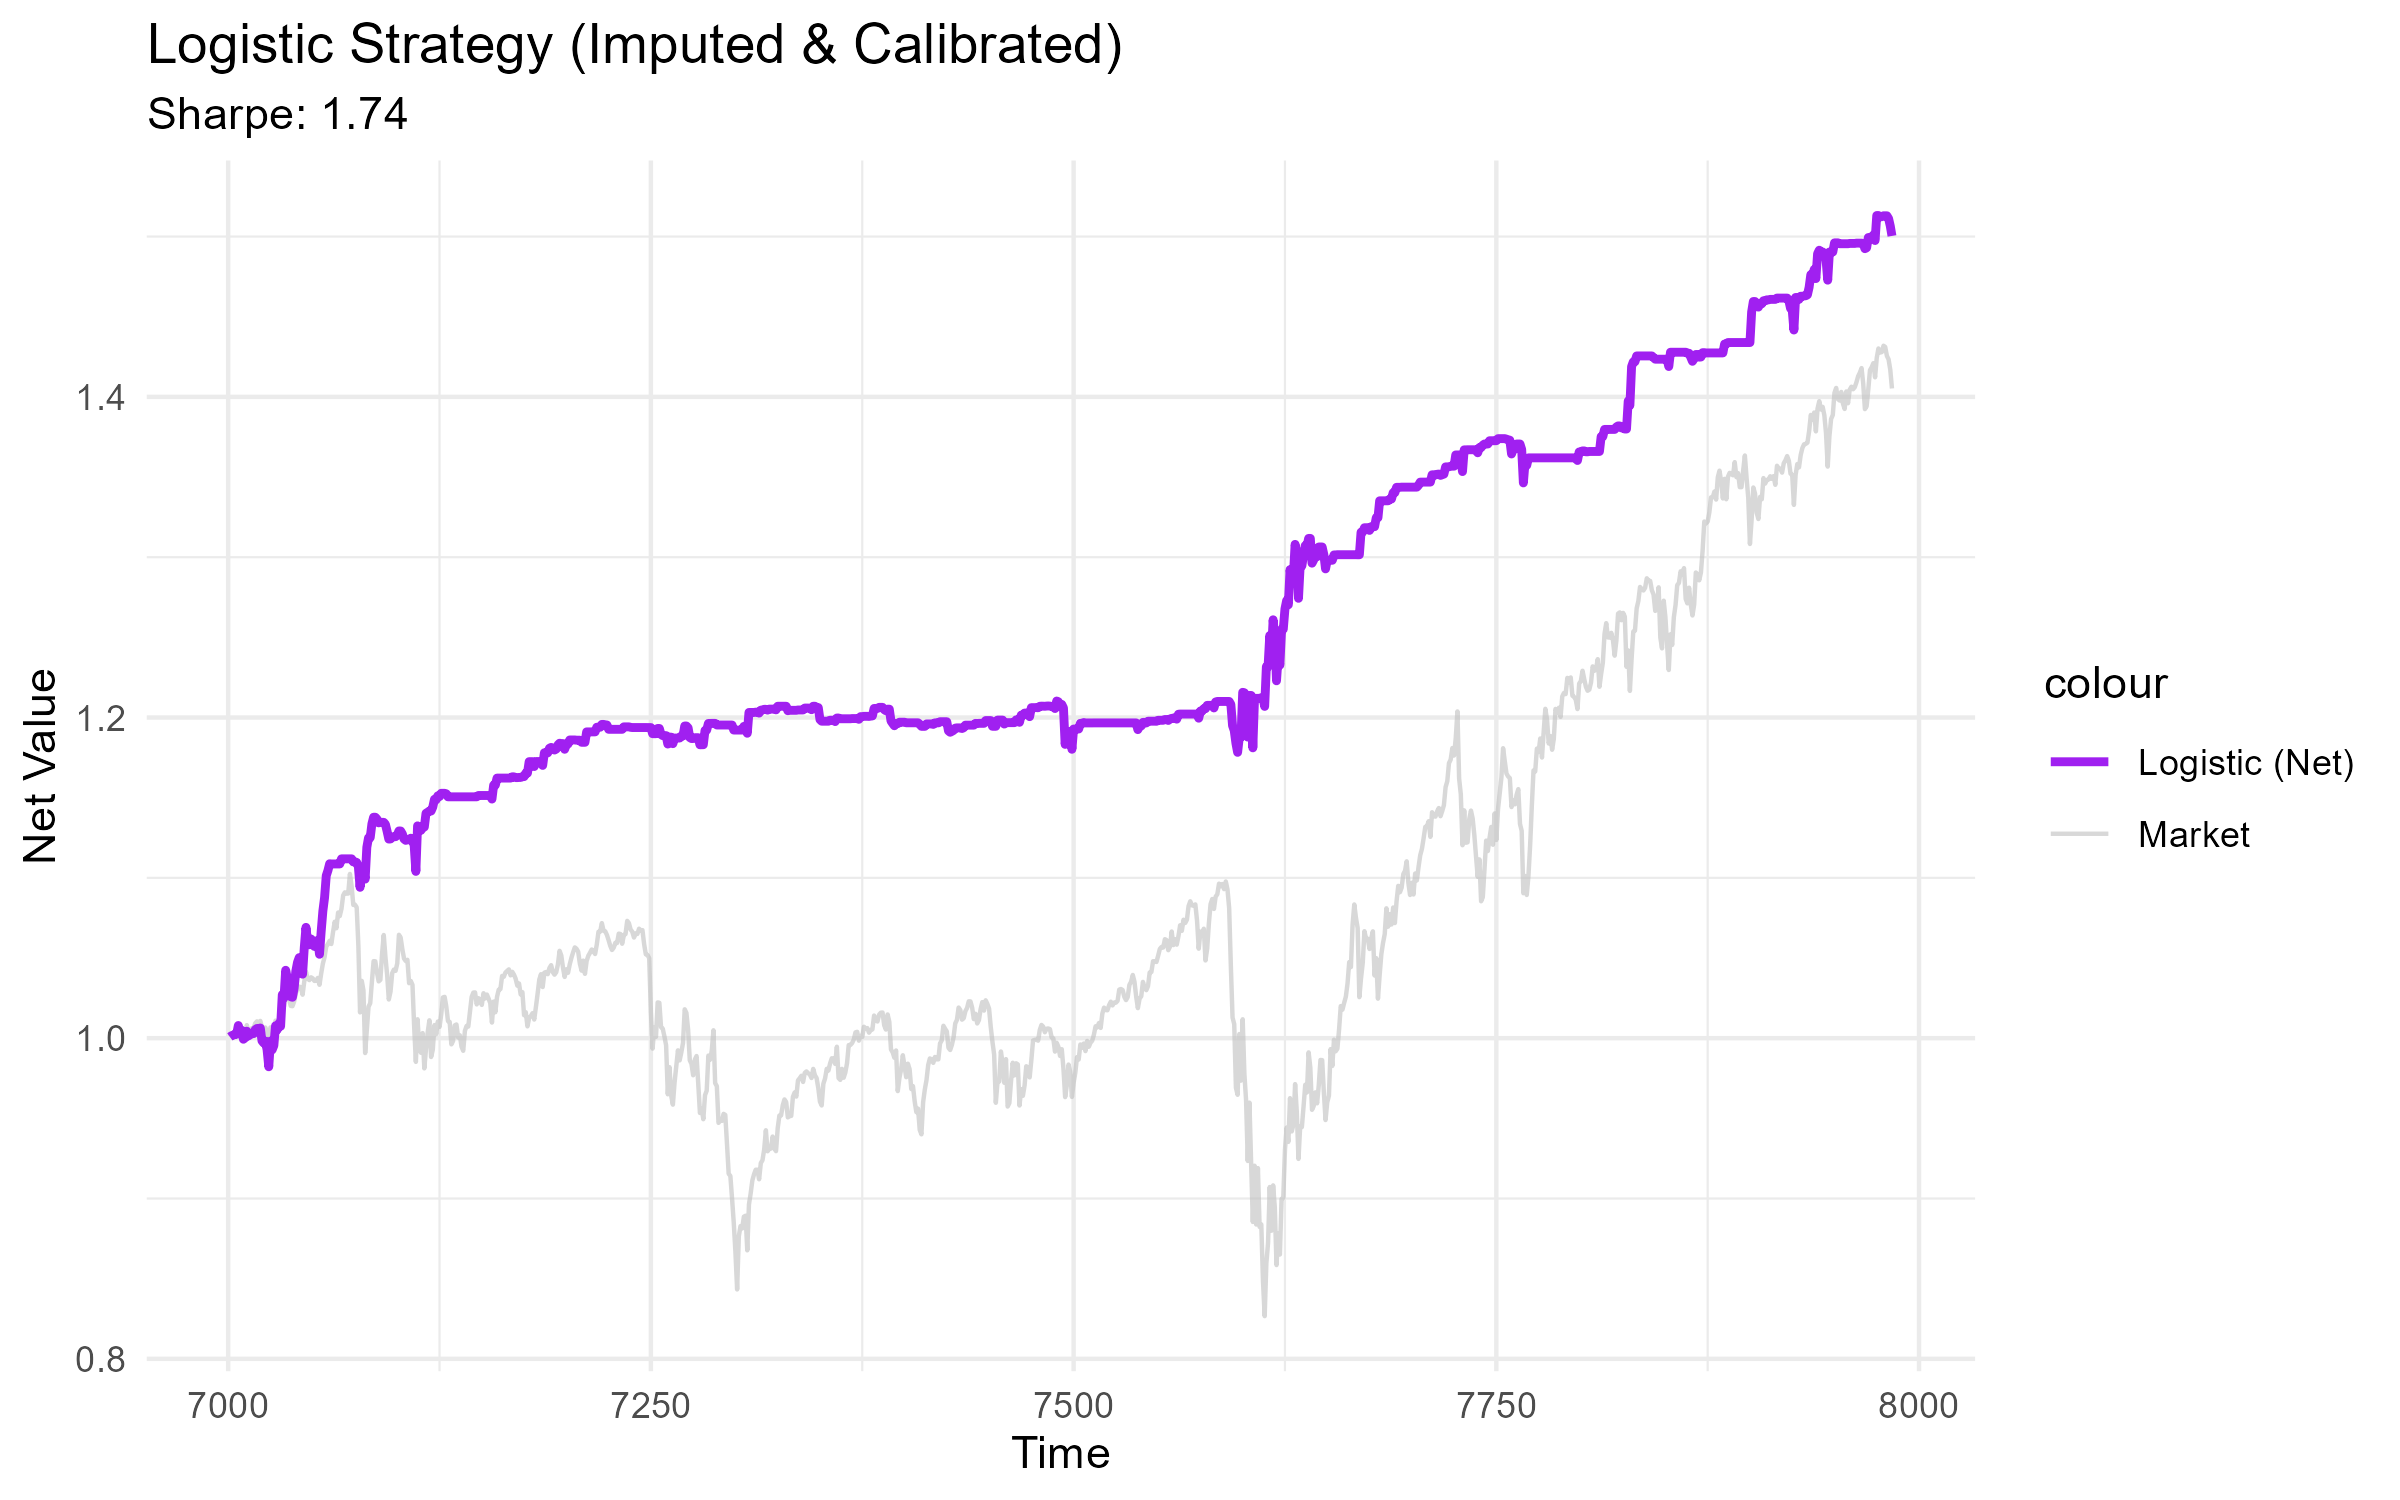
\includegraphics[width=\textwidth]{images/figure/logistic_equity_fixed_nocost.png}
        \caption{Logistic回归模型(不含交易费)}
    \end{subfigure}
    \hfill
    \begin{subfigure}[t]{0.31\textwidth}
        \centering
        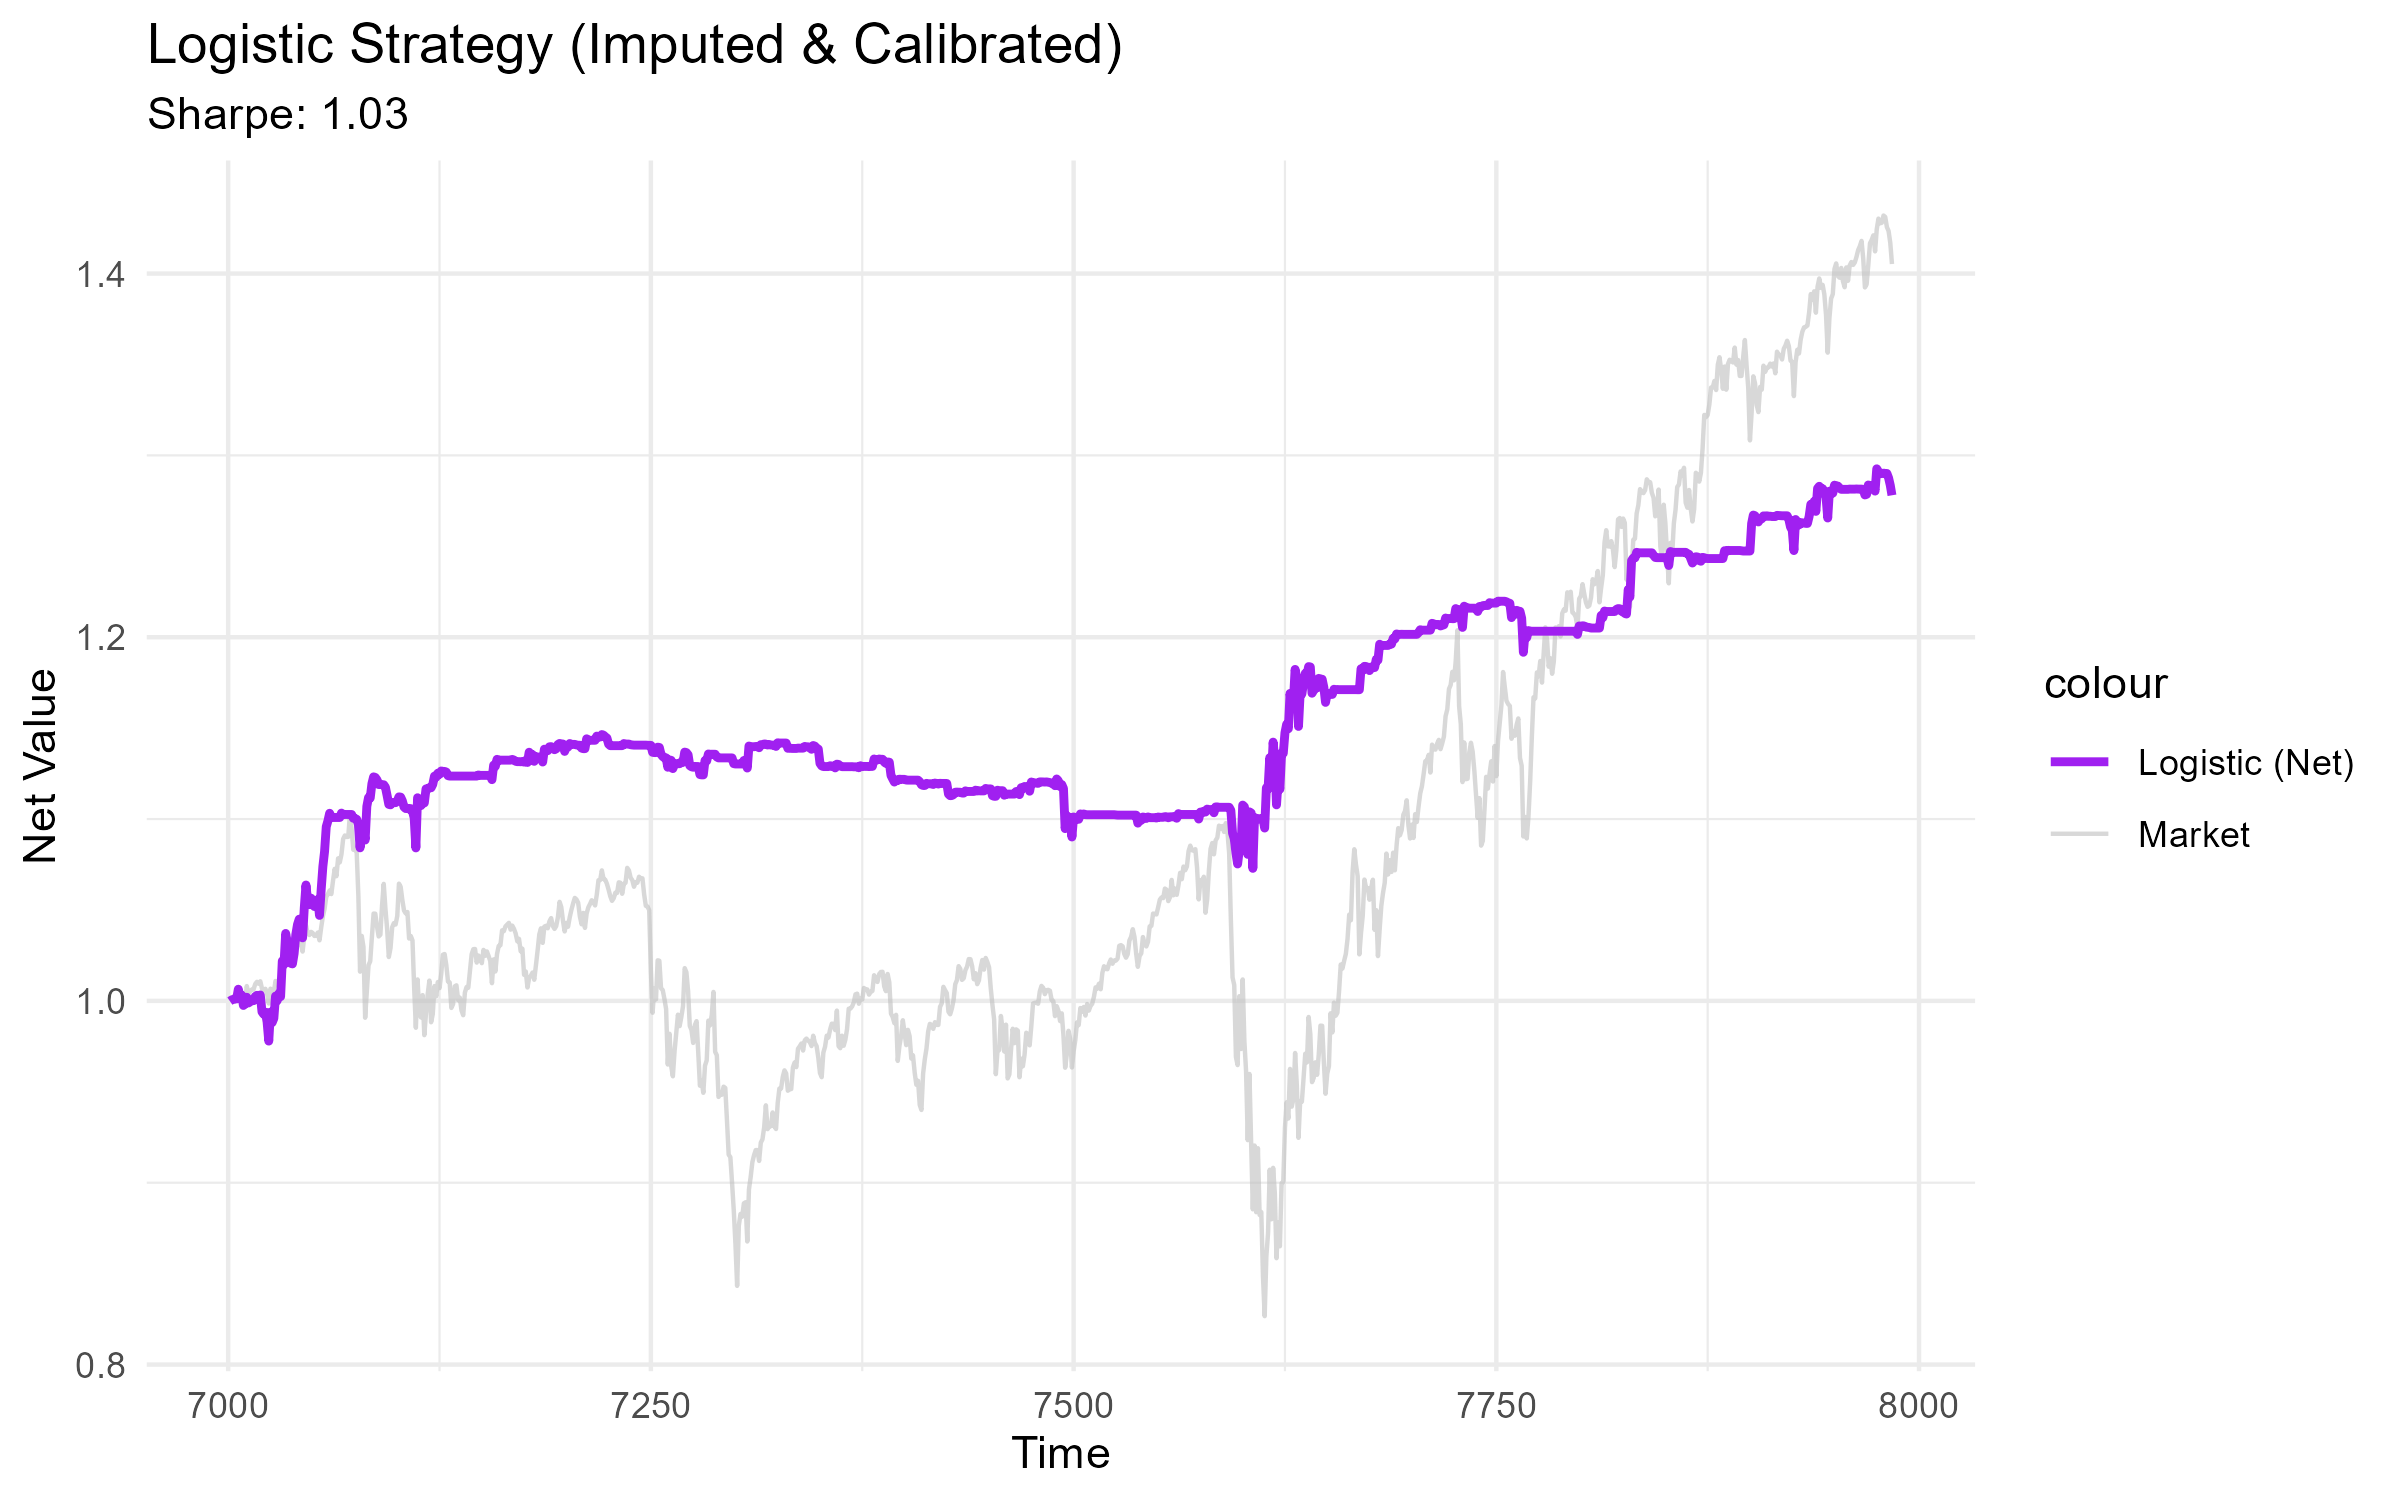
\includegraphics[width=\textwidth]{images/figure/logistic_equity_fixed.png}
        \caption{Logistic回归模型(含交易费)}
    \end{subfigure}
    \hfill
    \begin{subfigure}[t]{0.31\textwidth}
        \centering
        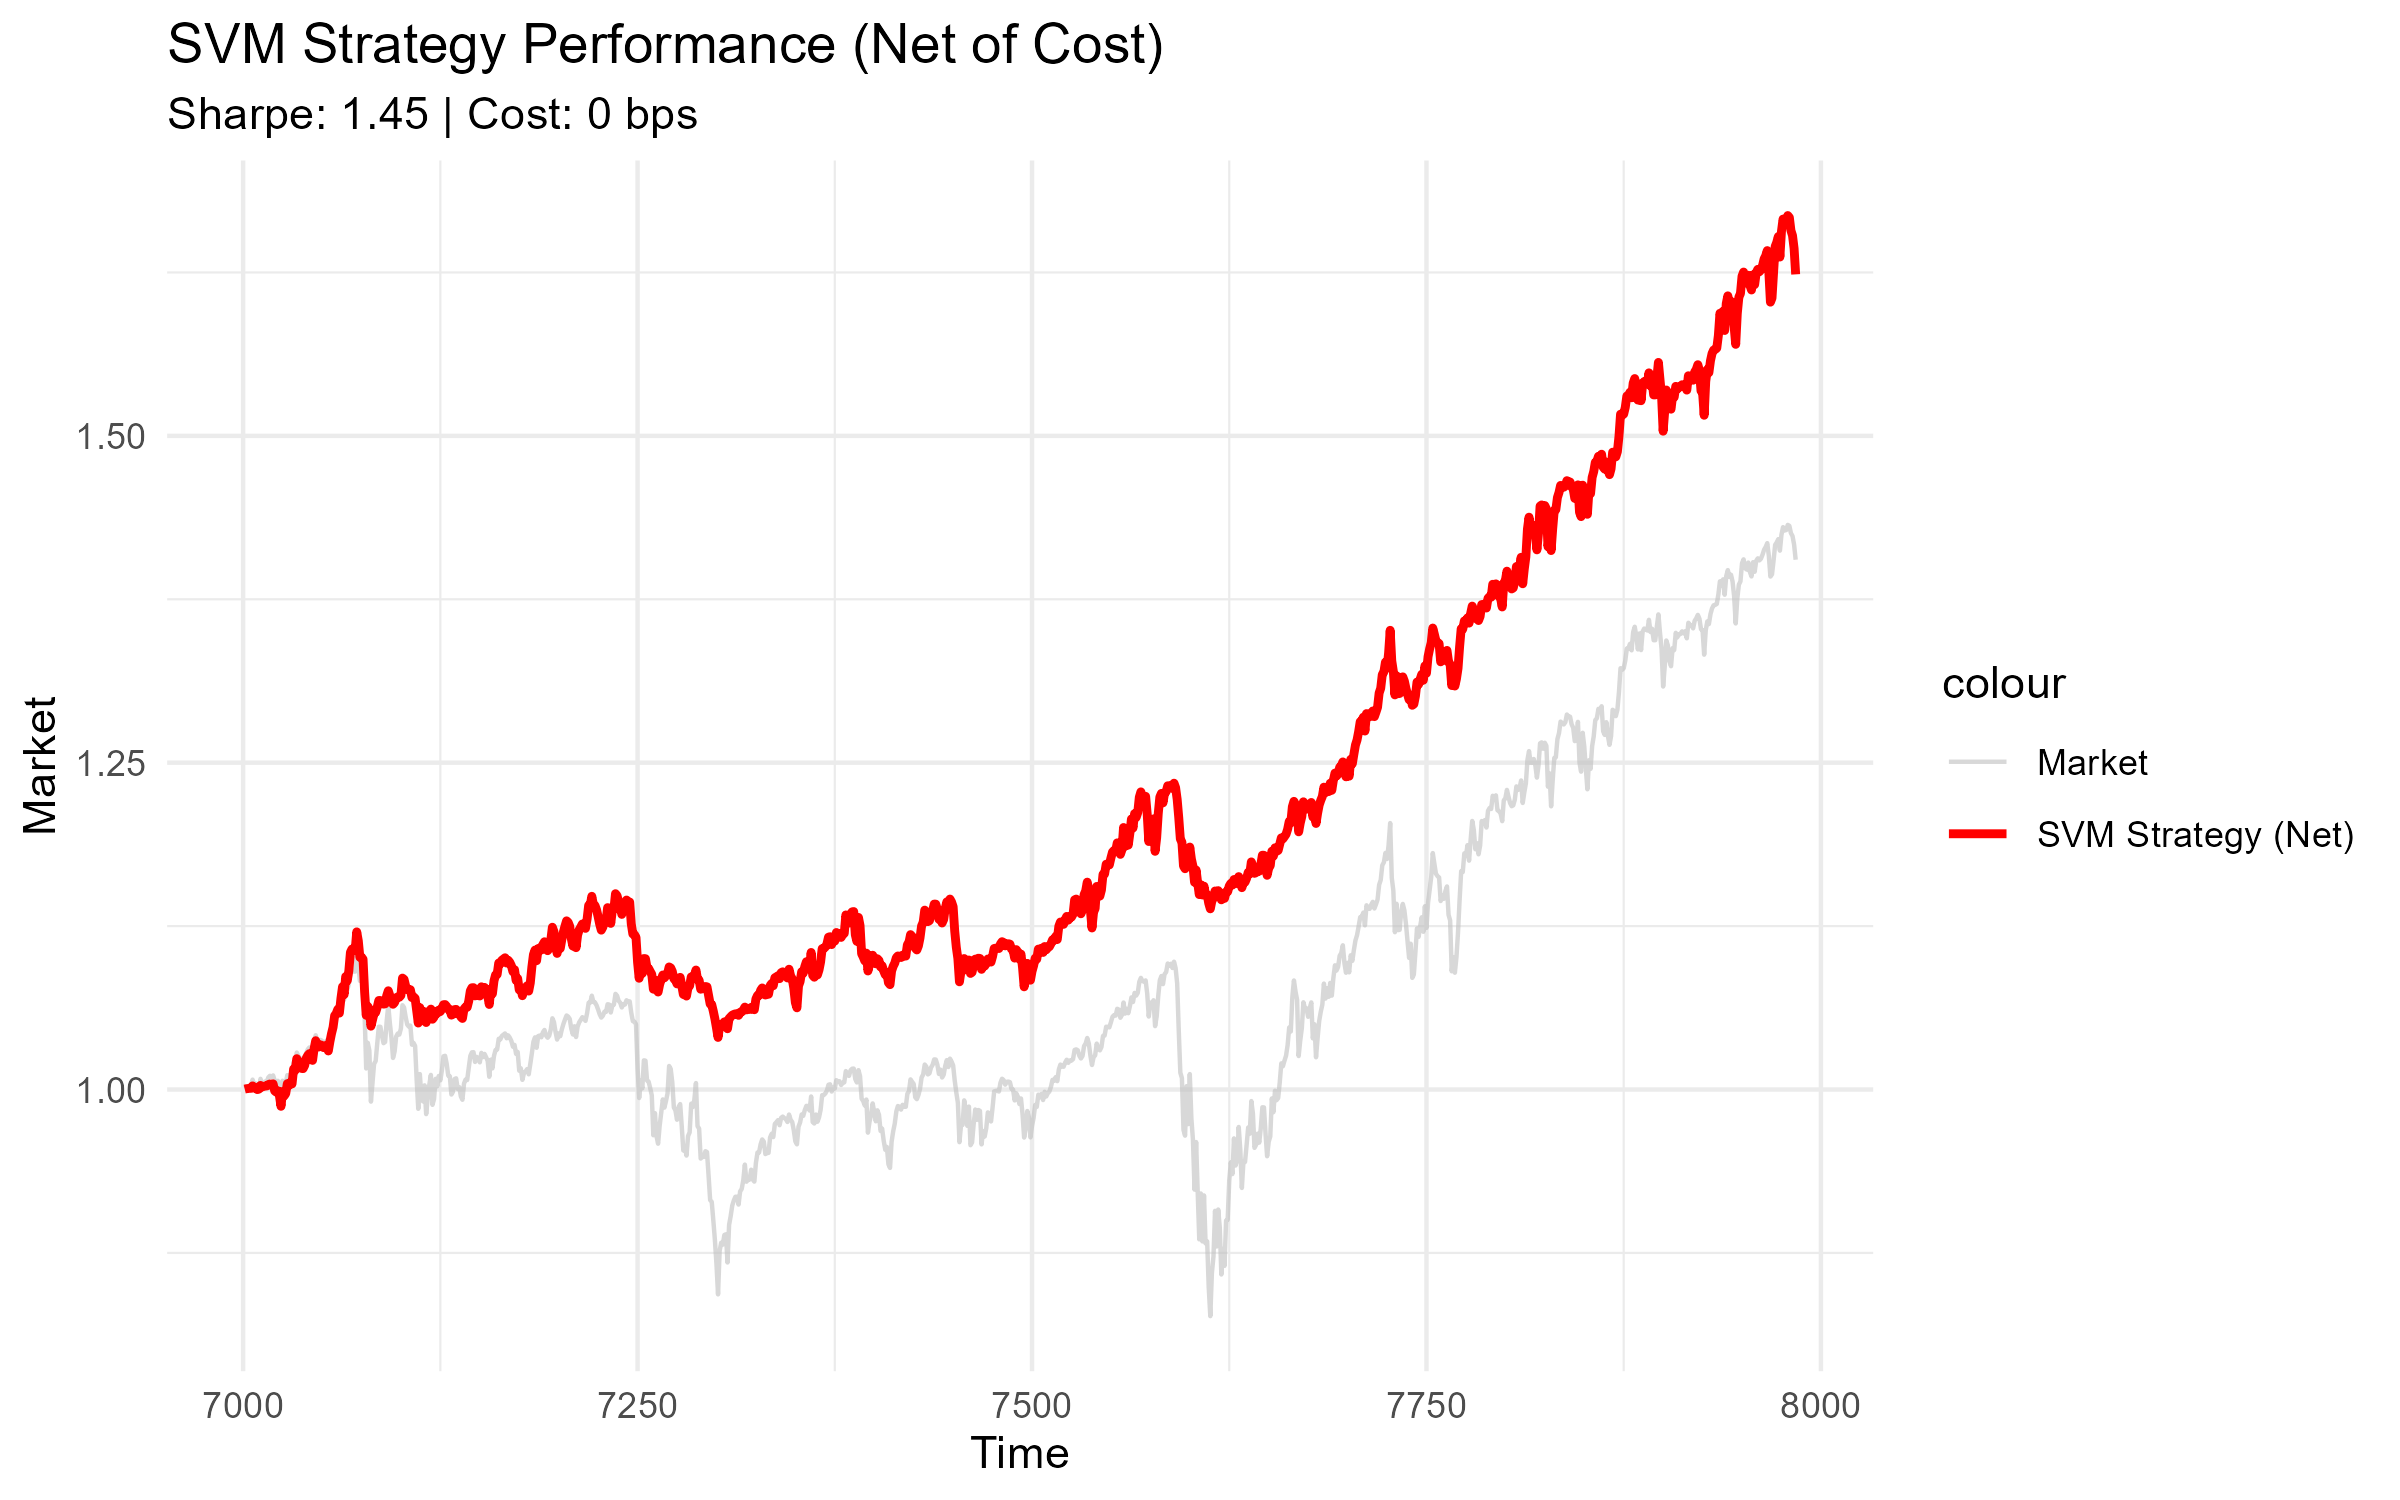
\includegraphics[width=\textwidth]{images/figure/equity_curve_nocost.png}
        \caption{SVM模型(不含交易费)}
    \end{subfigure}
    \vspace{0.2cm}

    \begin{subfigure}[t]{0.31\textwidth}
        \centering
        
\includegraphics[width=\textwidth]{images/figure/equity_curve.png}
        \caption{SVM模型(含交易费)}
    \end{subfigure}
    \hfill
    \begin{subfigure}[t]{0.31\textwidth}
        \centering
        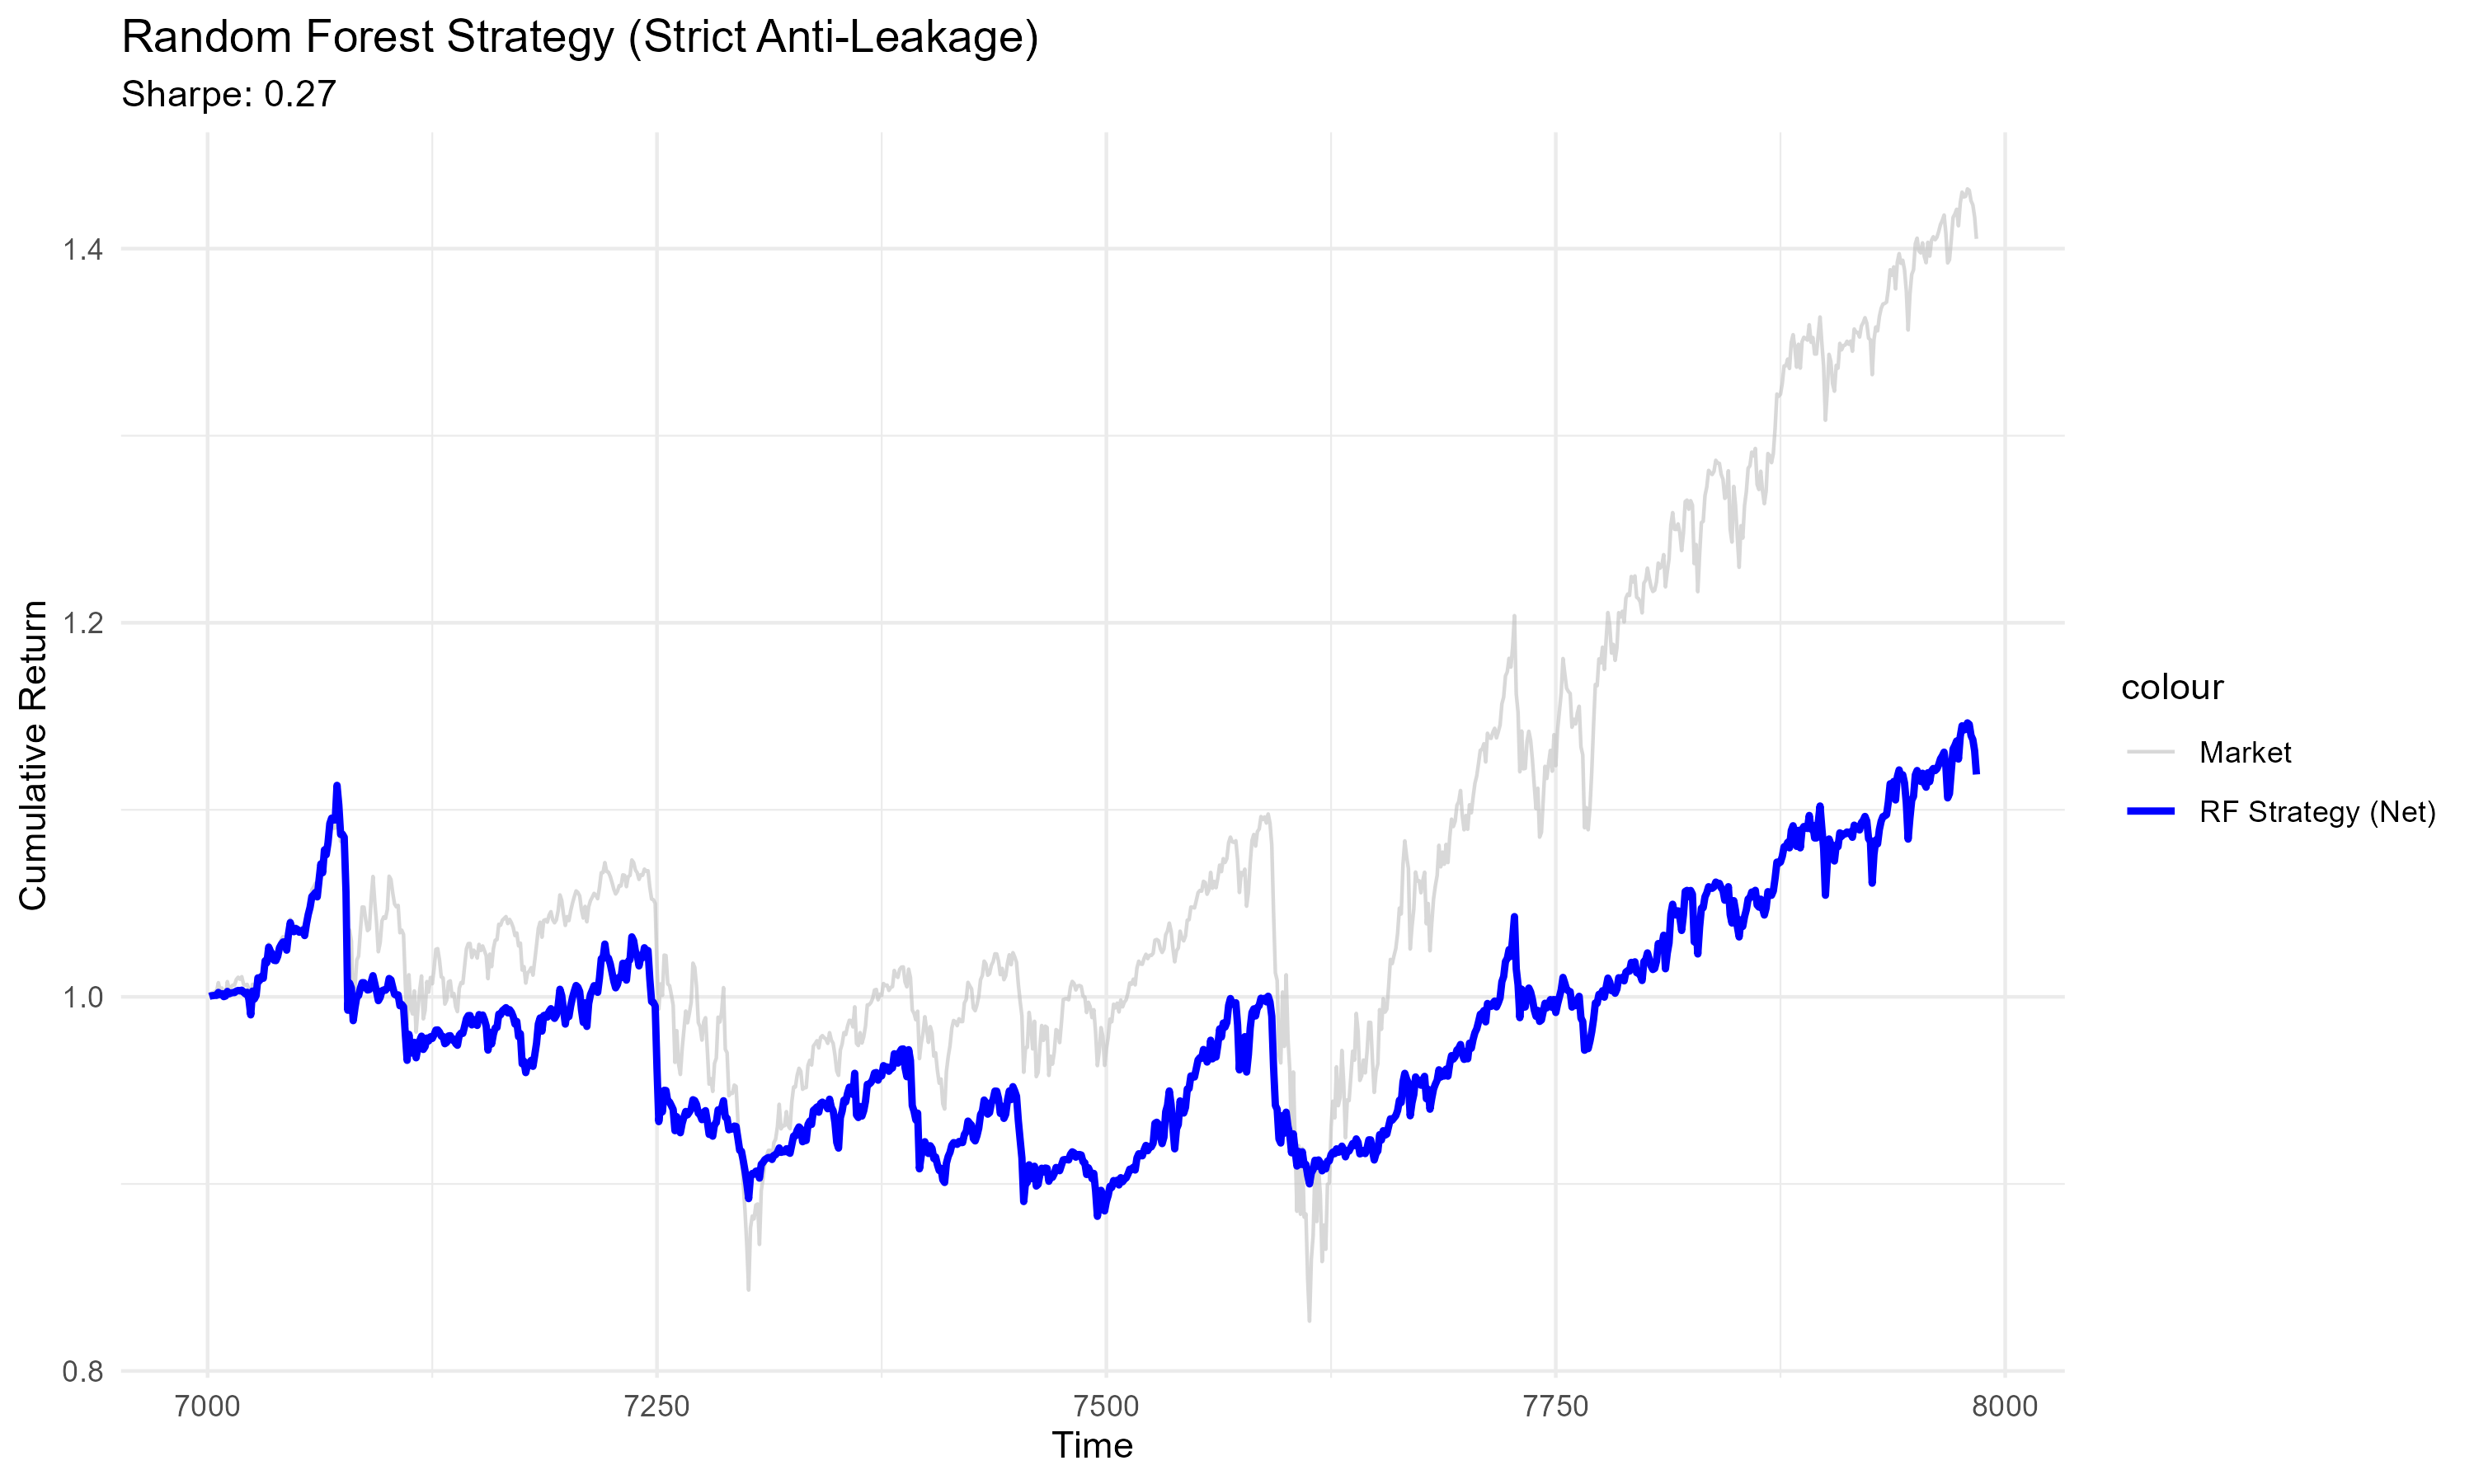
\includegraphics[width=\textwidth]{images/figure/rf_equity_curve_final_nocost.png}
        \caption{RF模型(不含交易费)}
    \end{subfigure}
    \hfill
    \begin{subfigure}[t]{0.31\textwidth}
        \centering
        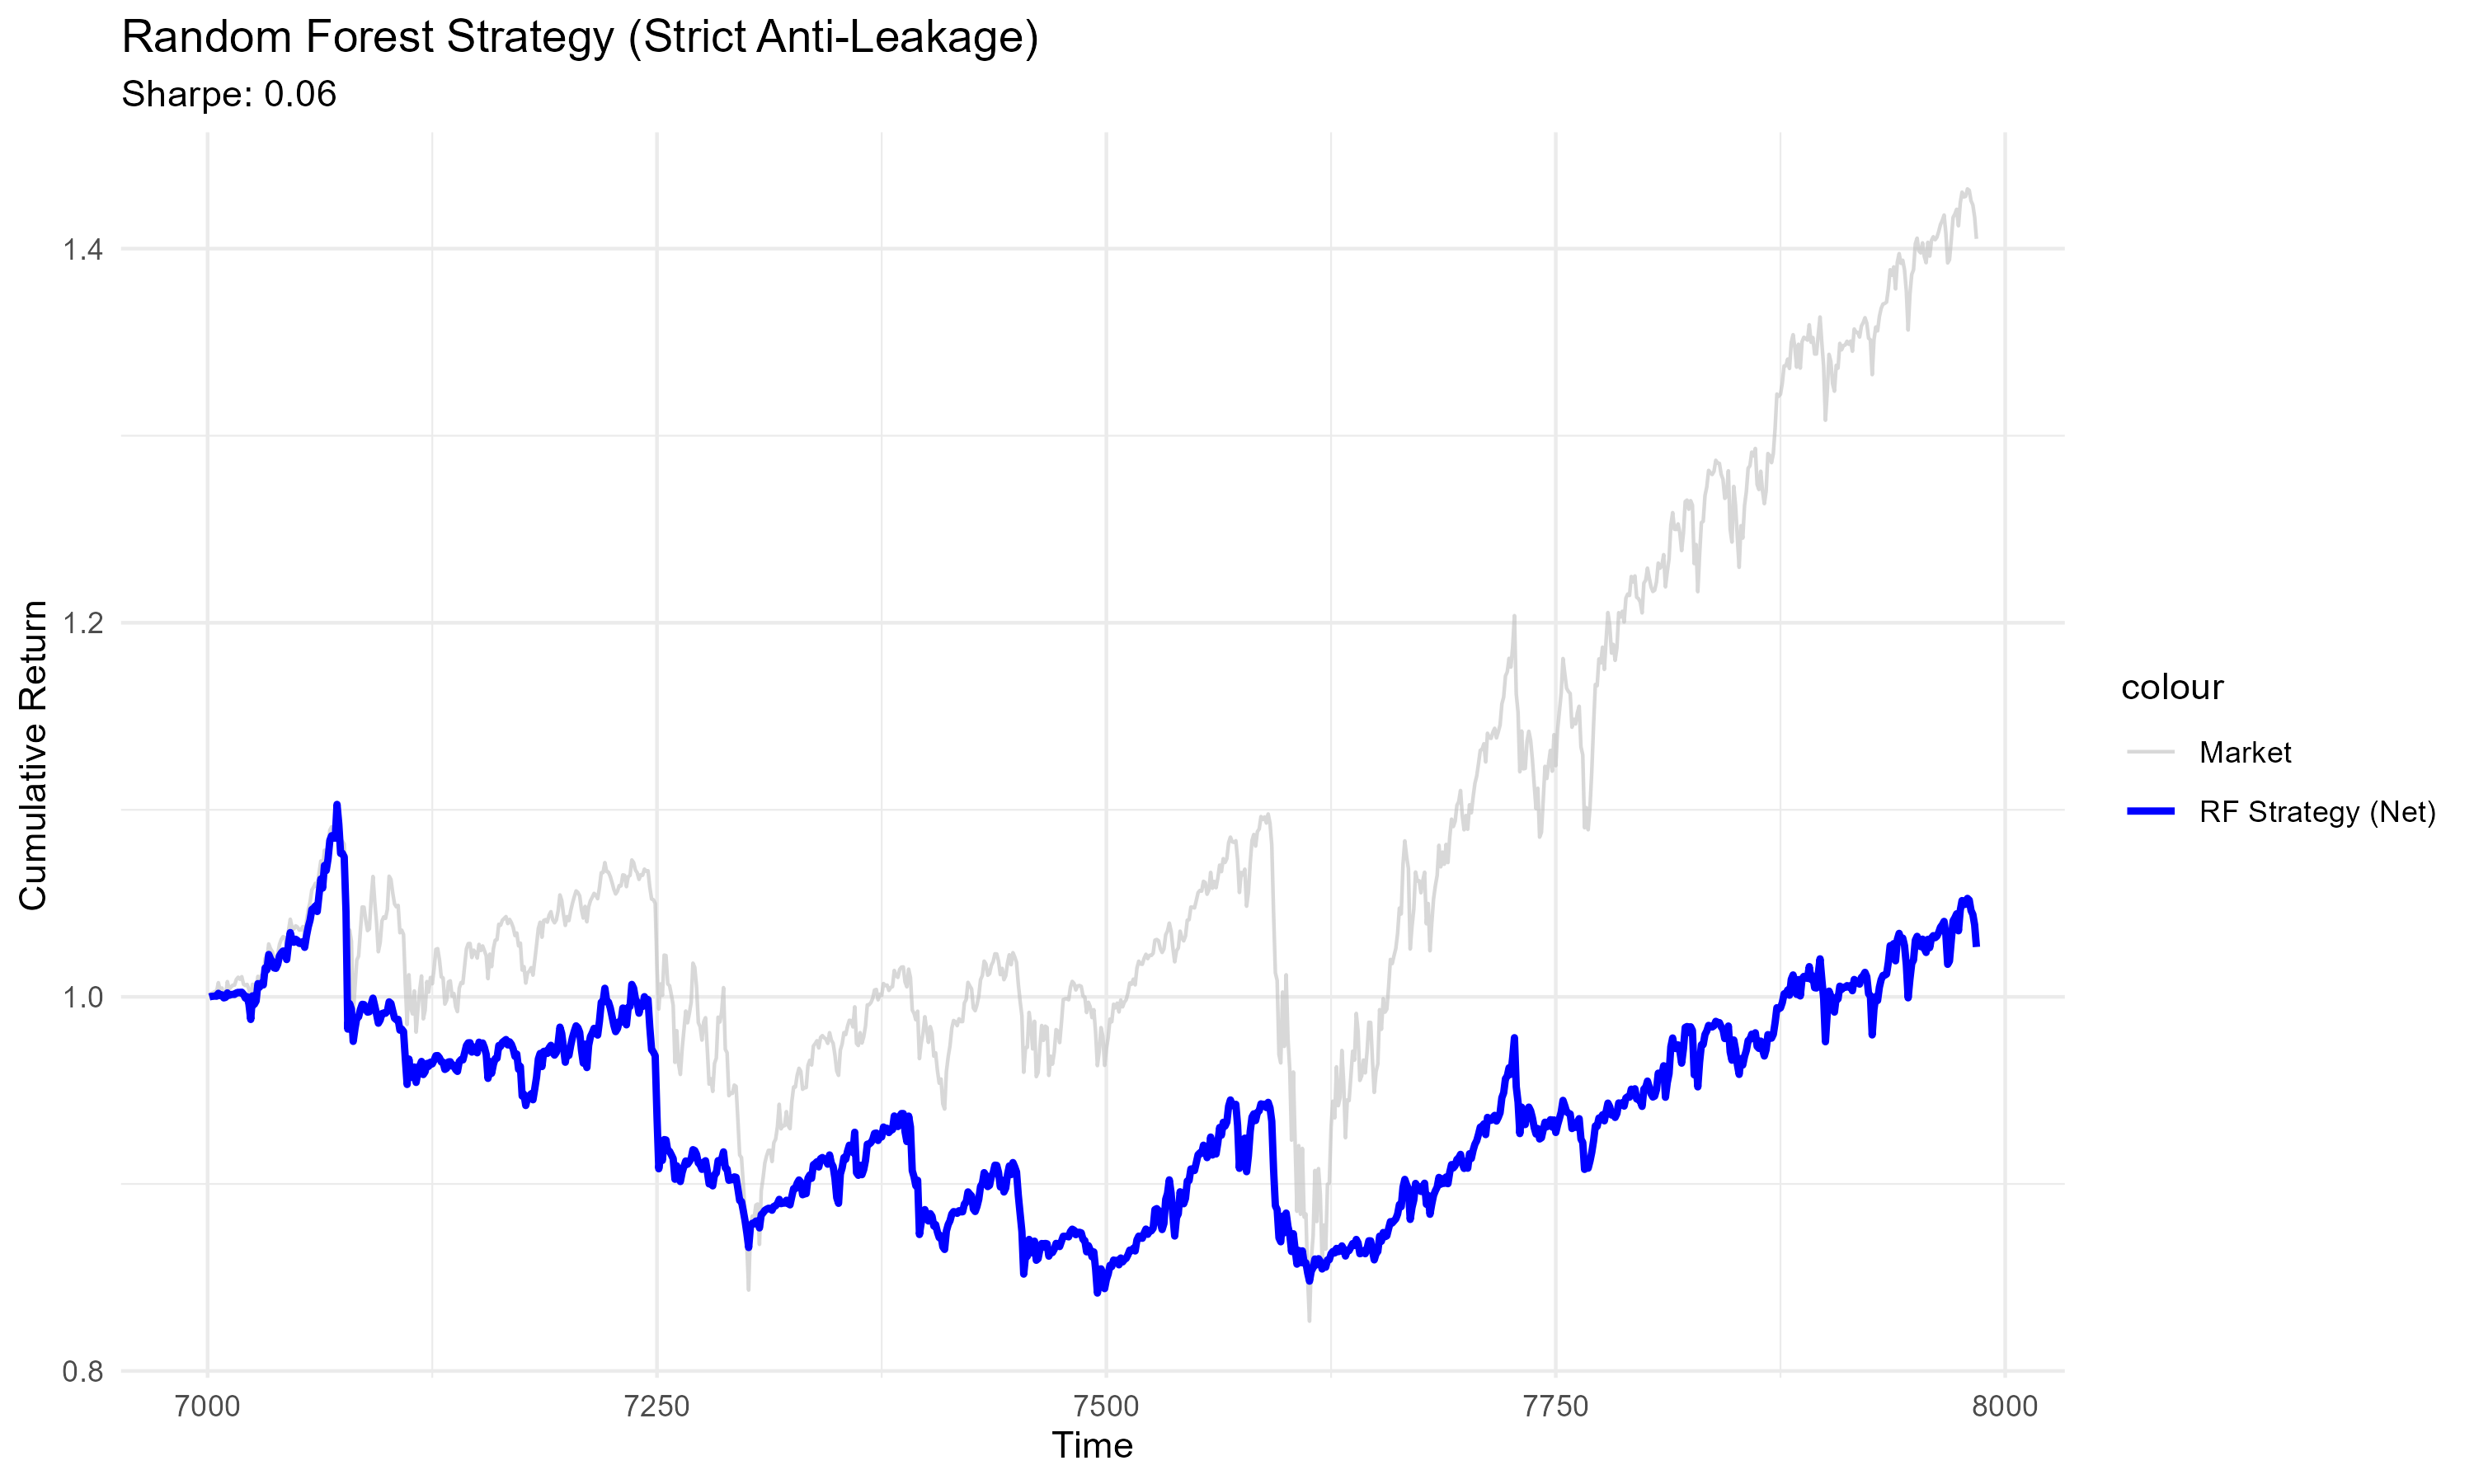
\includegraphics[width=\textwidth]{images/figure/rf_equity_curve_final.png}
        \caption{RF模型(含交易费)}
    \end{subfigure}
    \vspace{0.2cm}

    \begin{subfigure}[t]{0.31\textwidth}
        \centering
        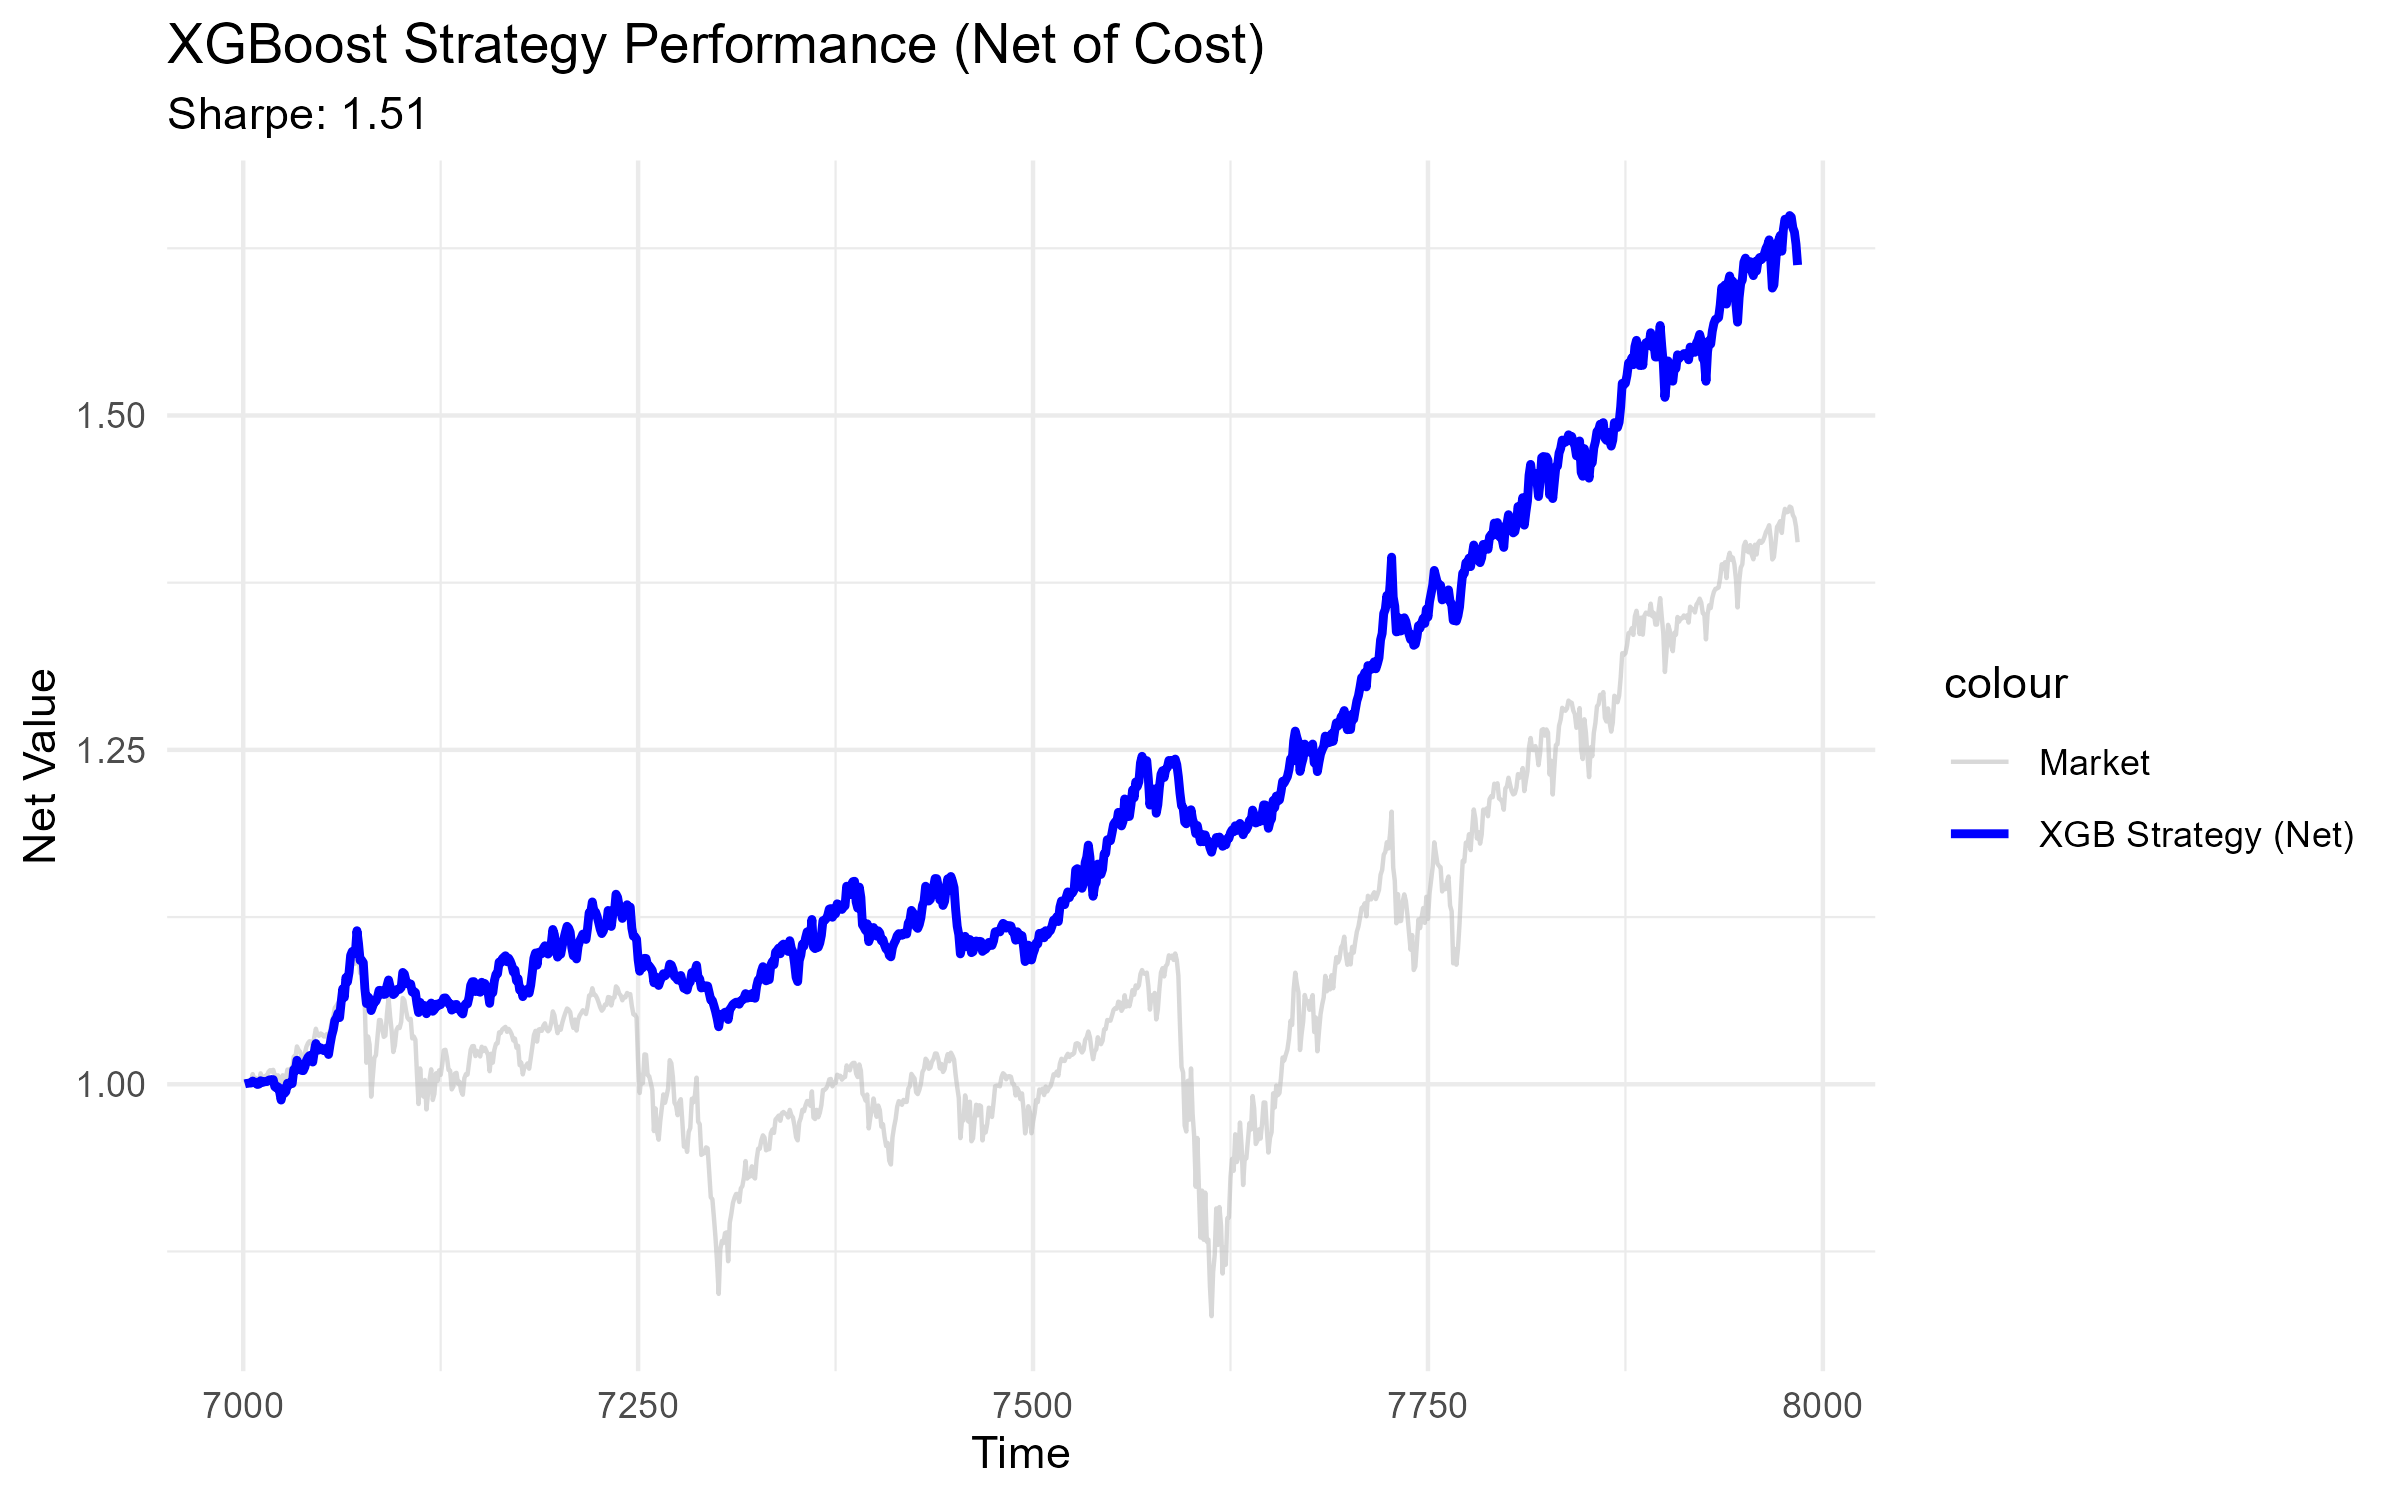
\includegraphics[width=\textwidth]{images/figure/xgb_equity_curve_nocost.png}
        \caption{XGB模型(不含交易费)}
    \end{subfigure}
    \hfill
    \begin{subfigure}[t]{0.31\textwidth}
        \centering
        
\includegraphics[width=\textwidth]{images/figure/xgb_equity_curve.png}
        \caption{XGB模型(含交易费)}
    \end{subfigure}
    % 为了对齐，第三个位置放一个空的minipage占位，或者直接留空
    \hfill
    \begin{subfigure}[t]{0.31\textwidth}
        \centering
        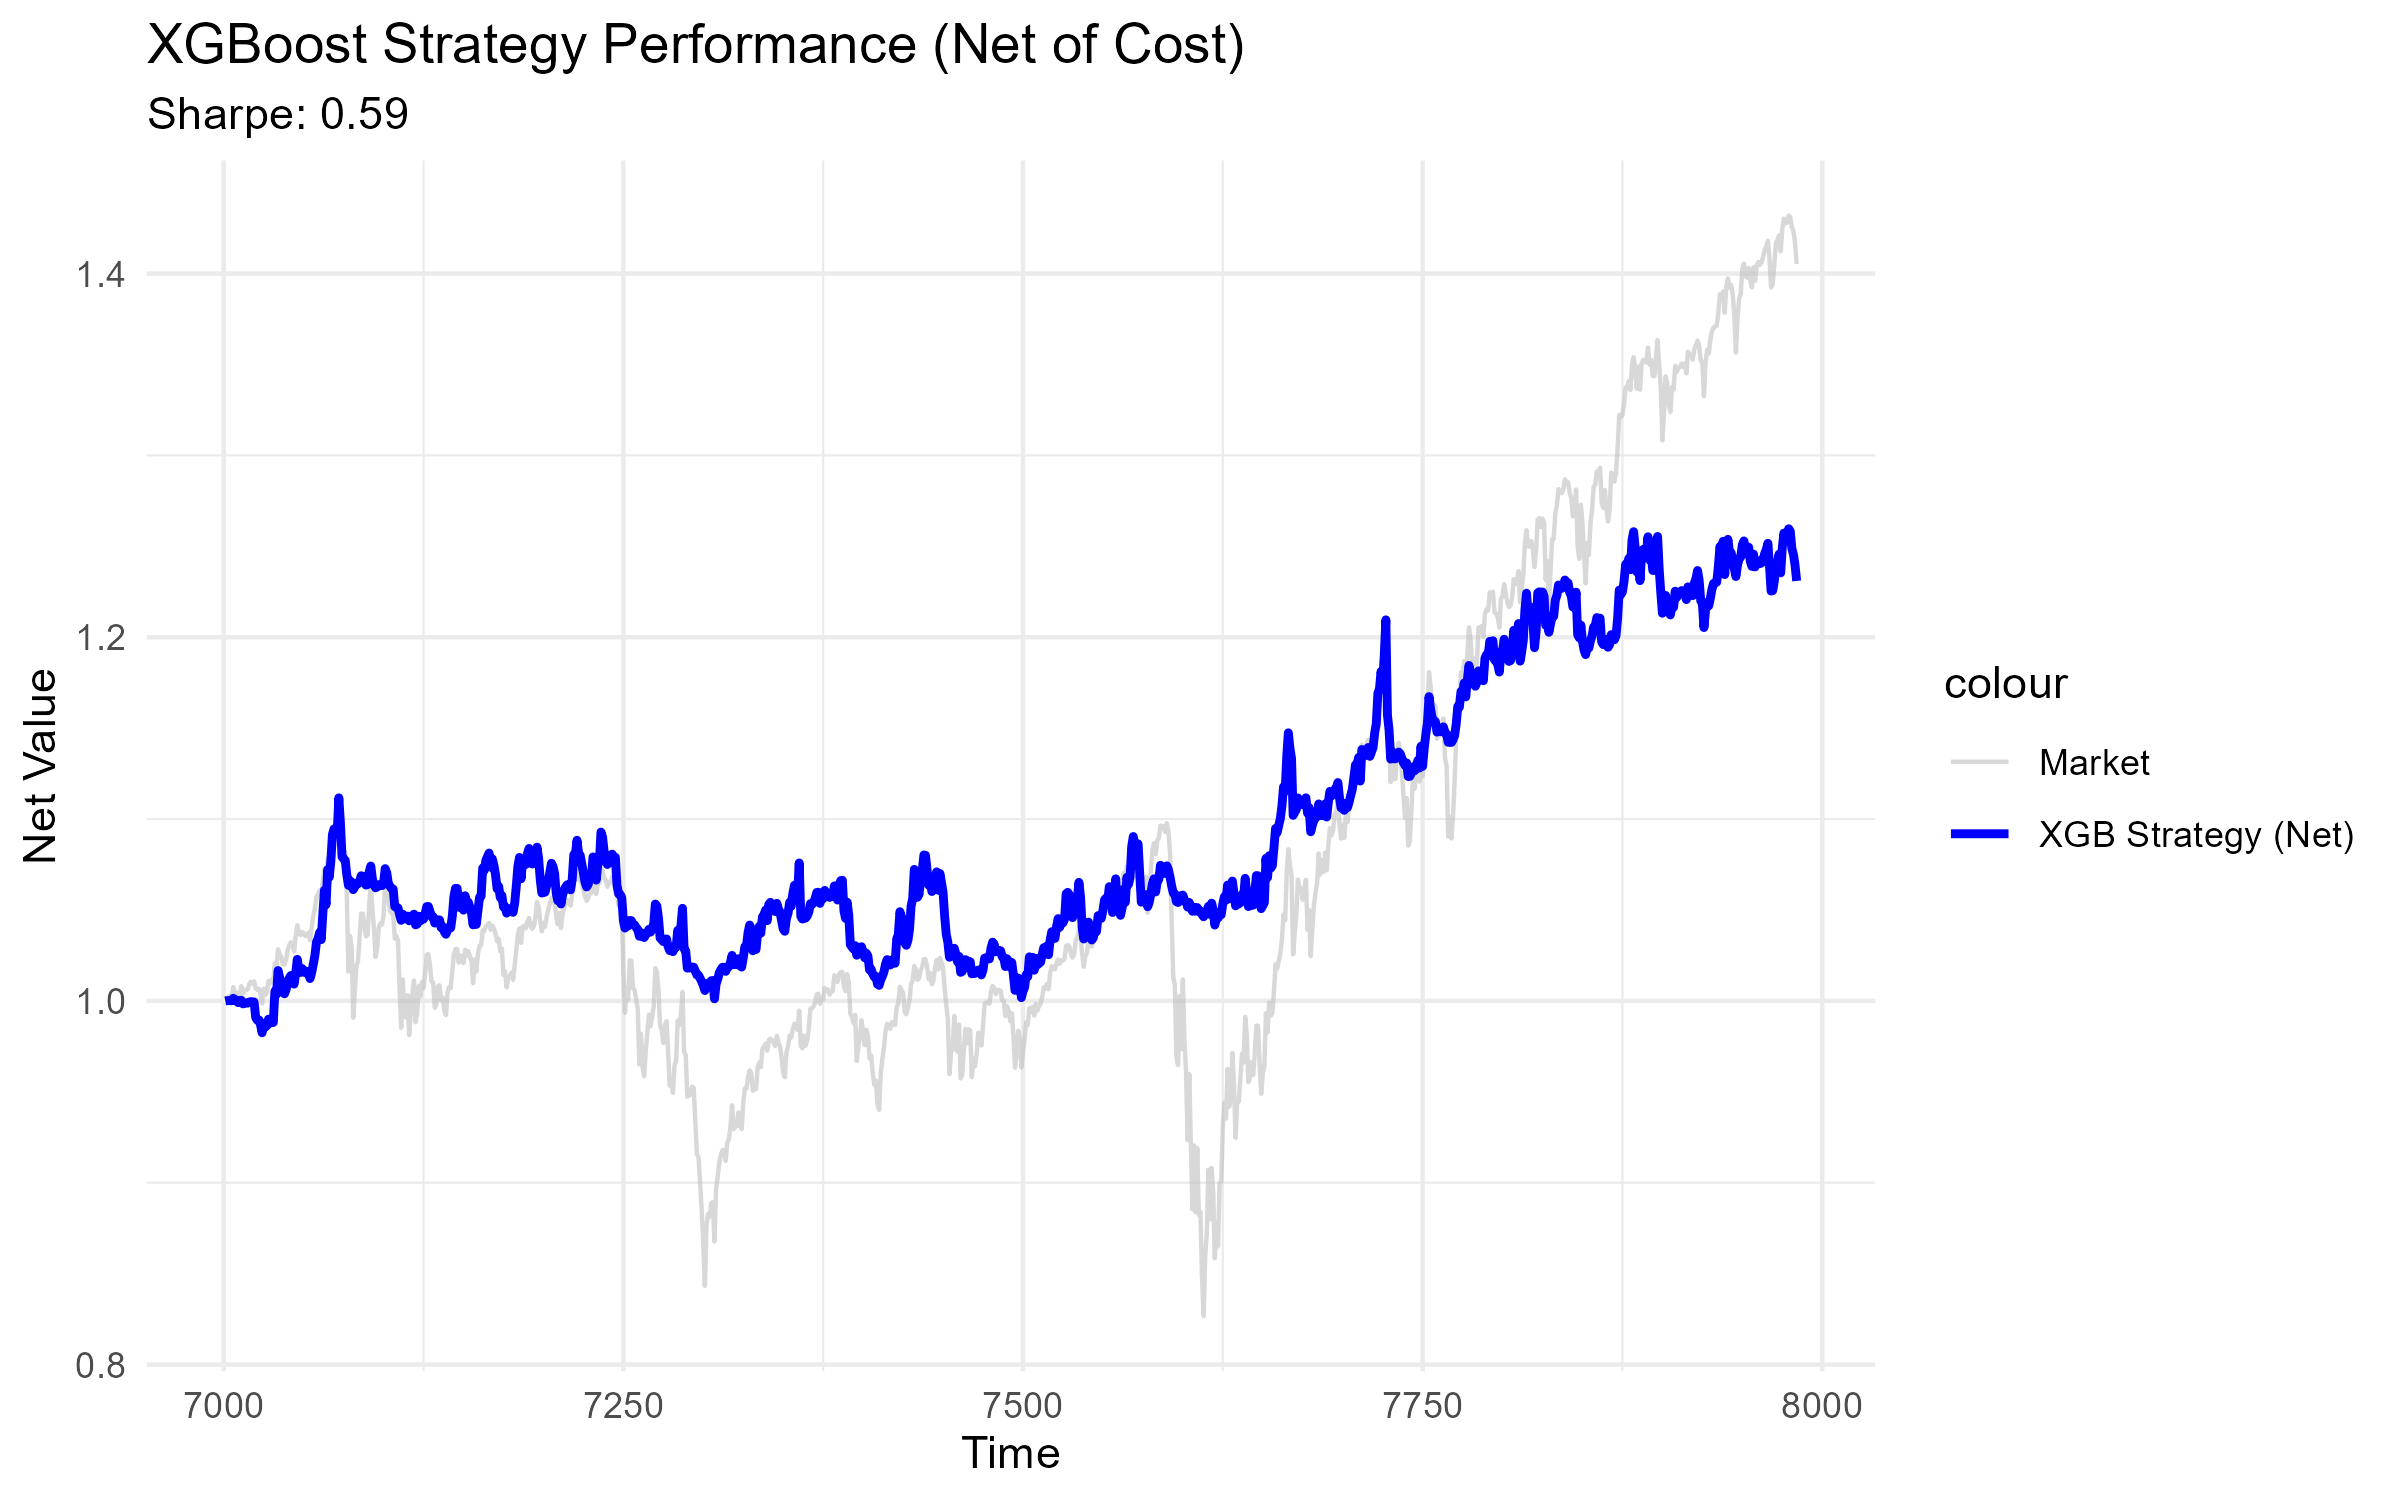
\includegraphics[width=\textwidth]{images/figure/xgb_equity_curve_lasso.png}
        \caption{XGB模型(含交易费,Lasso)}
    \end{subfigure}

    \begin{subfigure}[t]{0.31\textwidth}
        \centering
        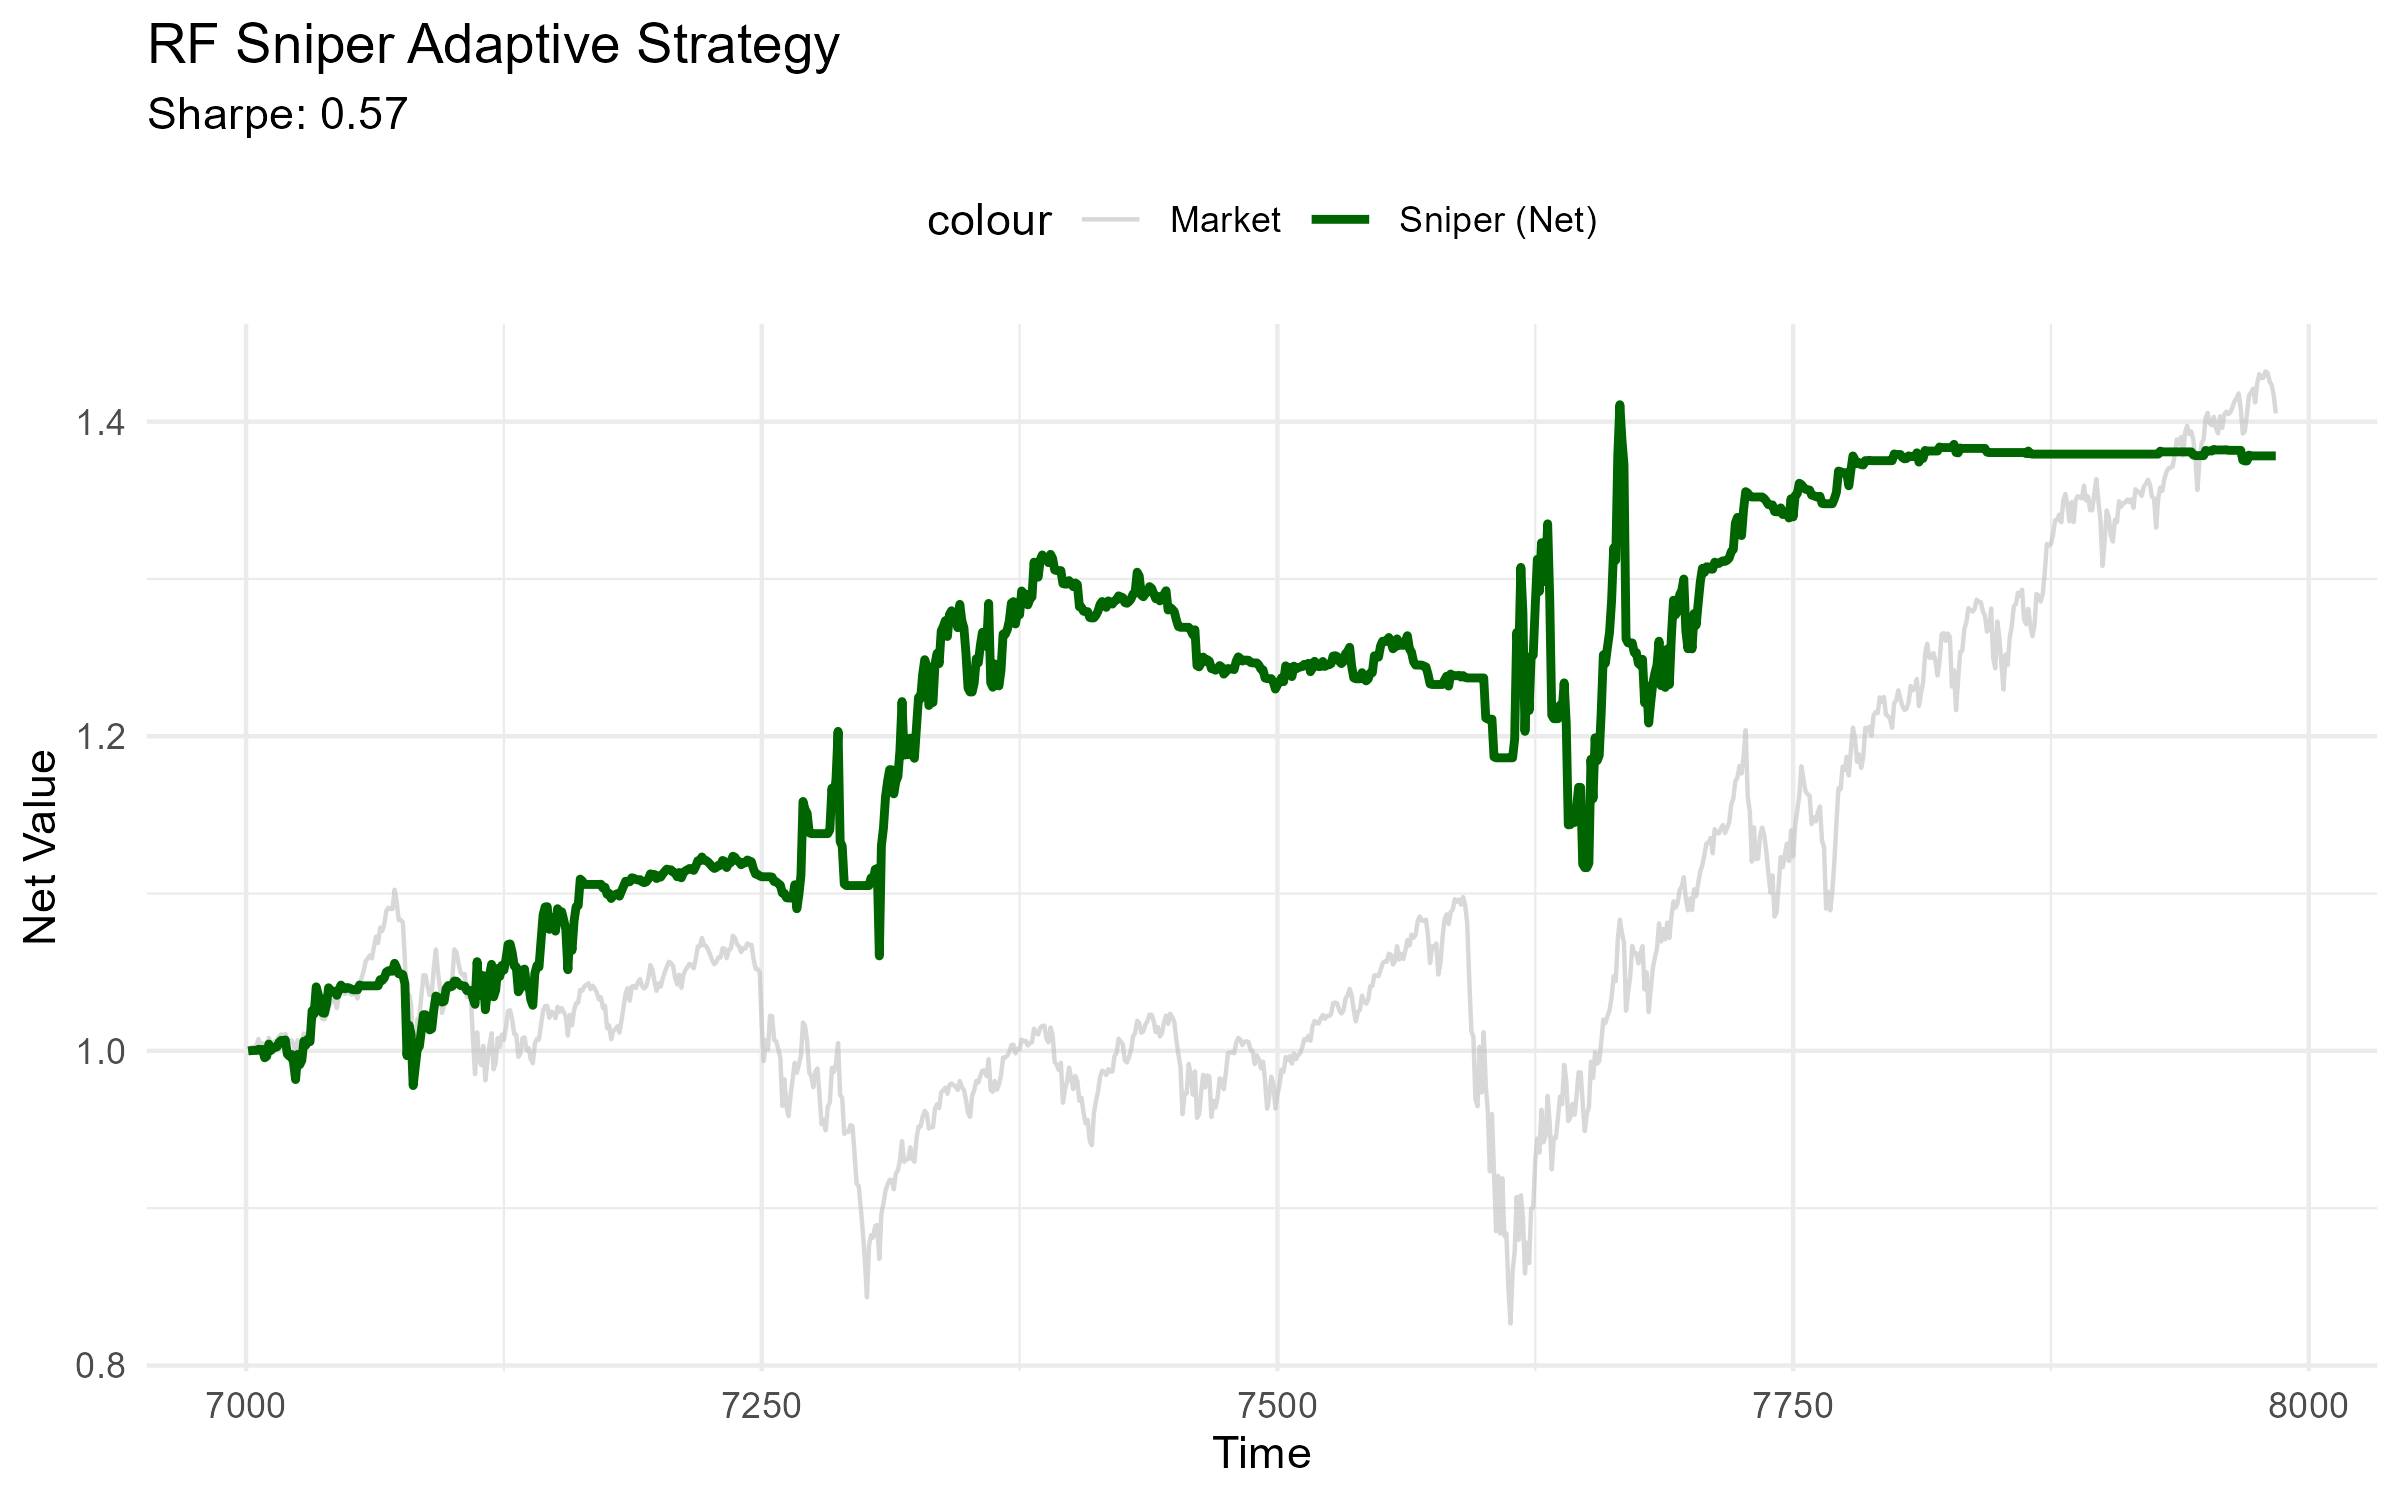
\includegraphics[width=\textwidth]{images/figure/rf_sniper_equity.png}
        \caption{RF新策略} 
    \end{subfigure}
    
    \caption{所有模型回测表现对比}
\end{figure}
\clearpage
\begin{figure}[htbp]
  \centering
  
  % --- 第一张小图 ---
  \begin{subfigure}[b]{0.49\textwidth} % 宽度设为页面宽度的45%
    \centering
    % 注意:这里 width=\linewidth 是指占满这个 subfigure 的宽度,不是整页
    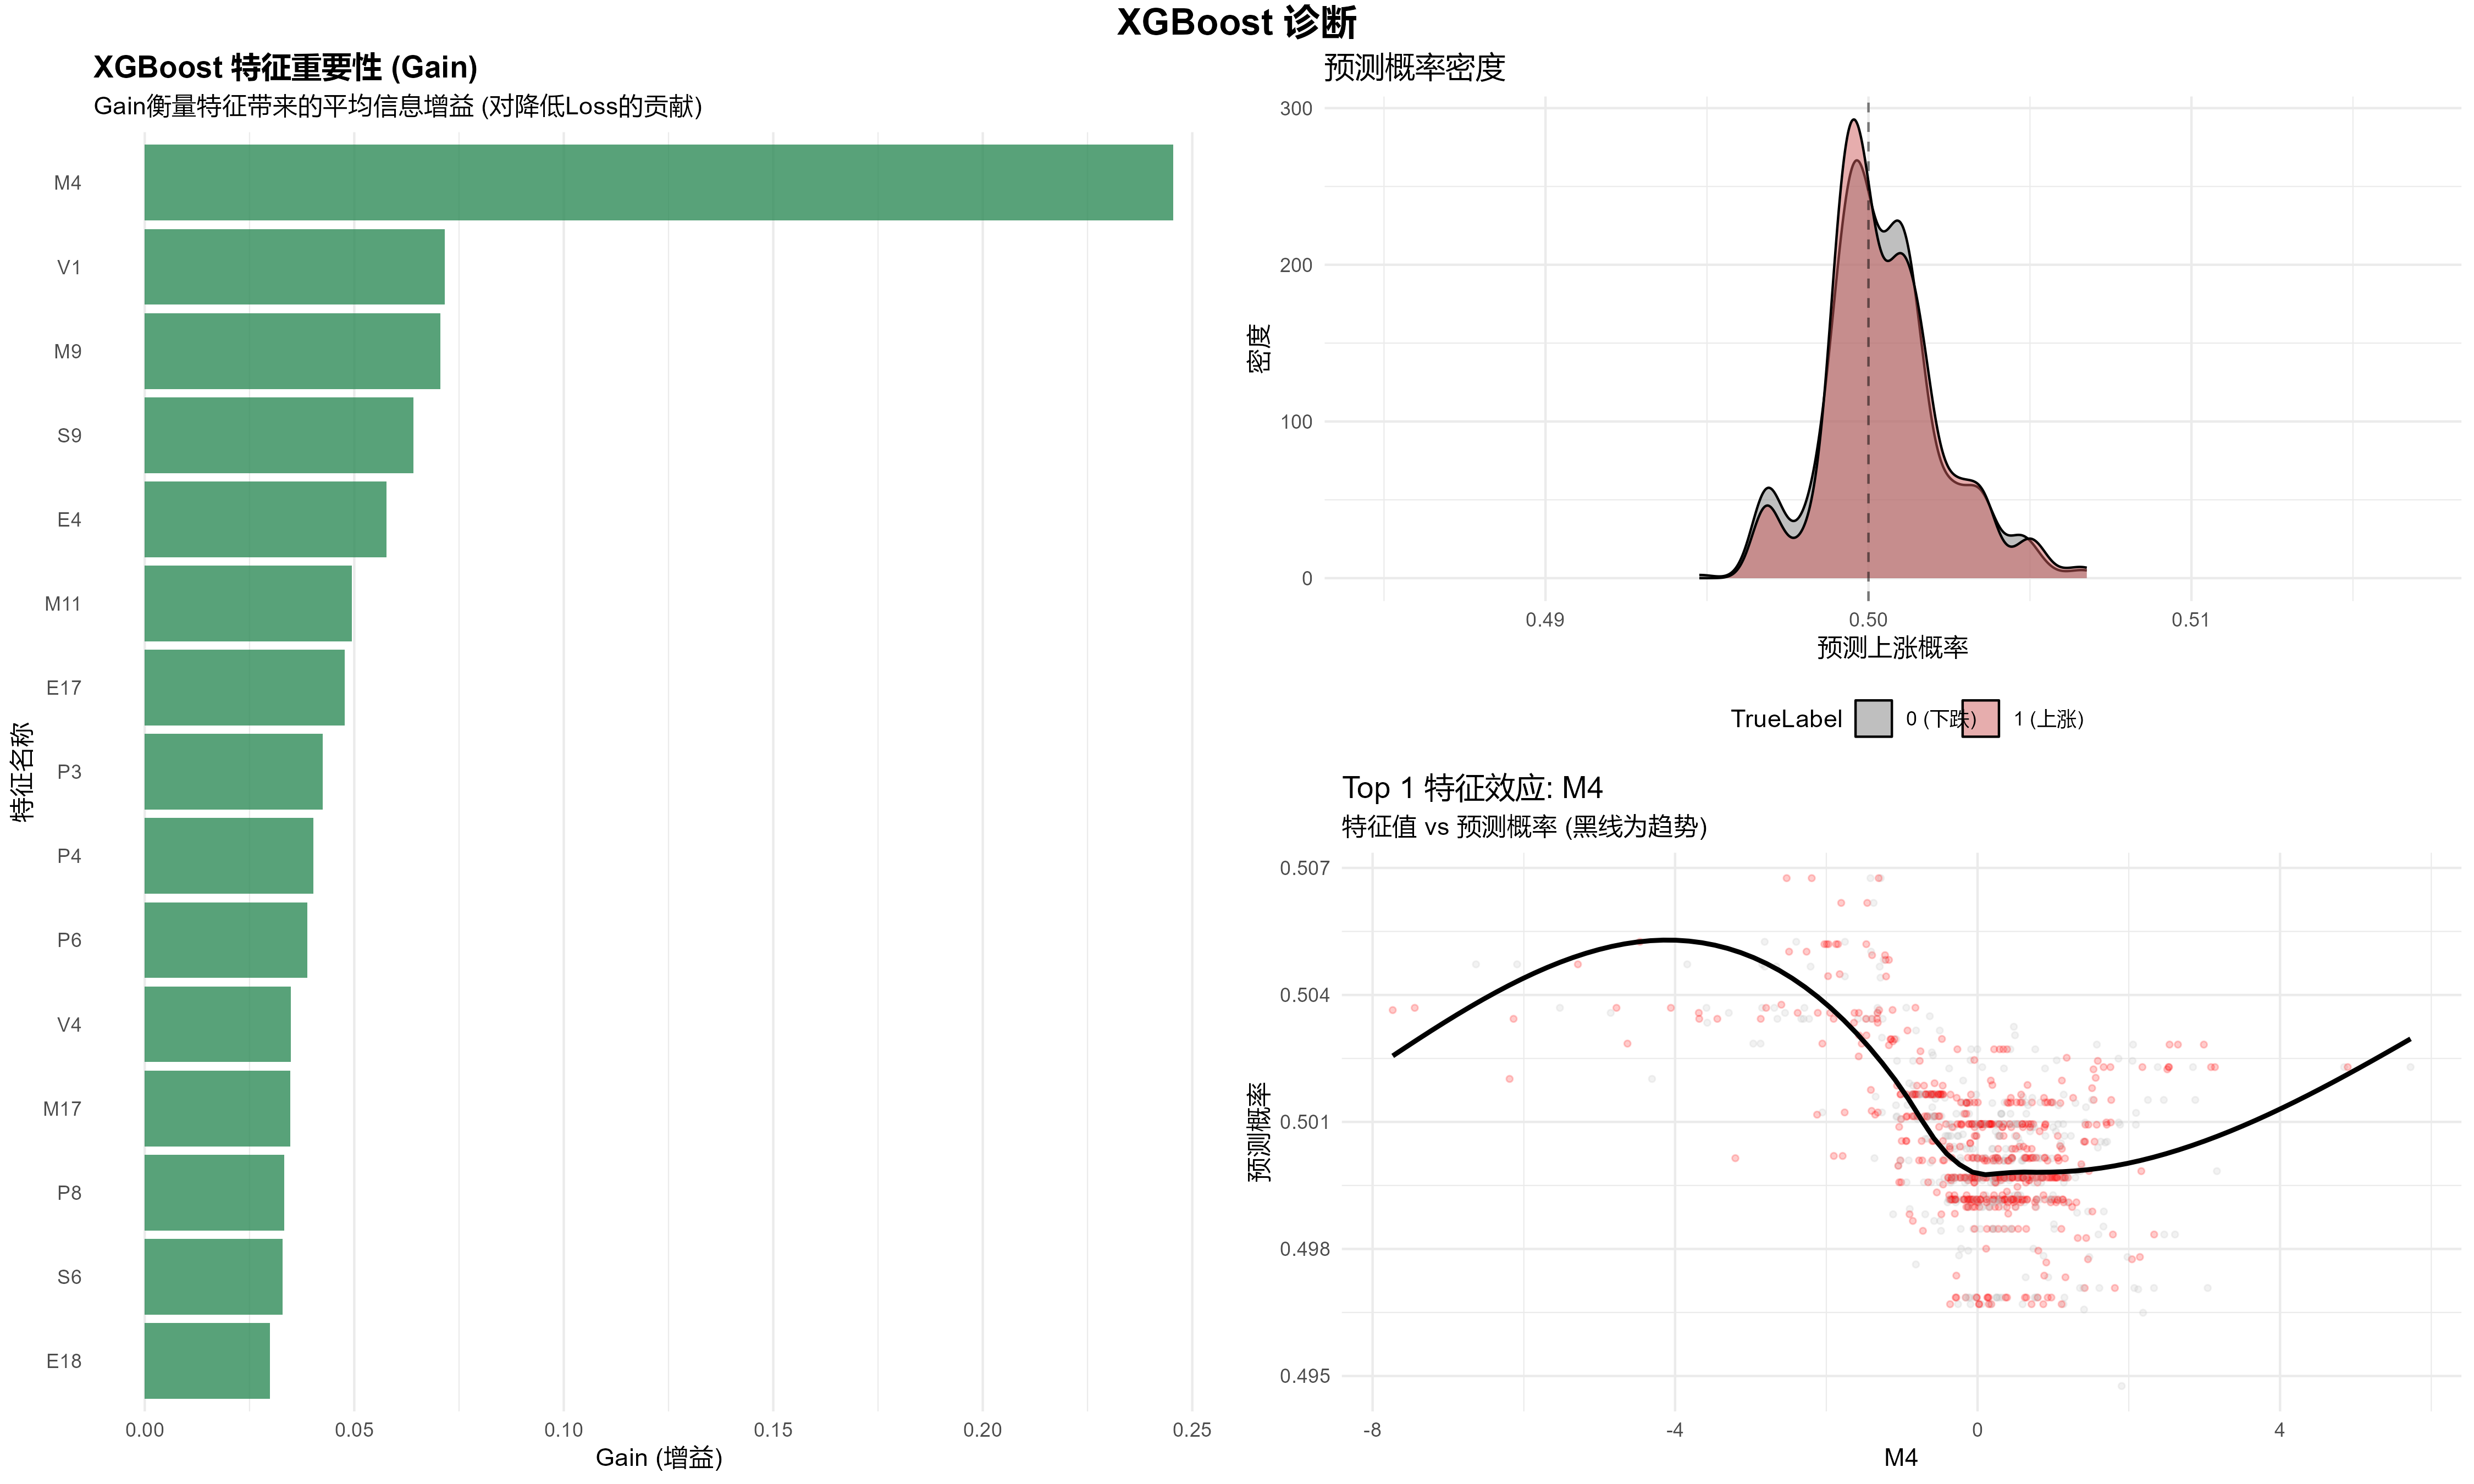
\includegraphics[width=\linewidth]{images/figure2/xgb_analysis_plot.png} 
    \caption{无Lasso处理}
    \label{fig:left}
  \end{subfigure}
  \hfill % 【关键】在两图之间弹簧填充,把它们挤到两边
  % --- 第二张小图 ---
  \begin{subfigure}[b]{0.49\textwidth}
    \centering
    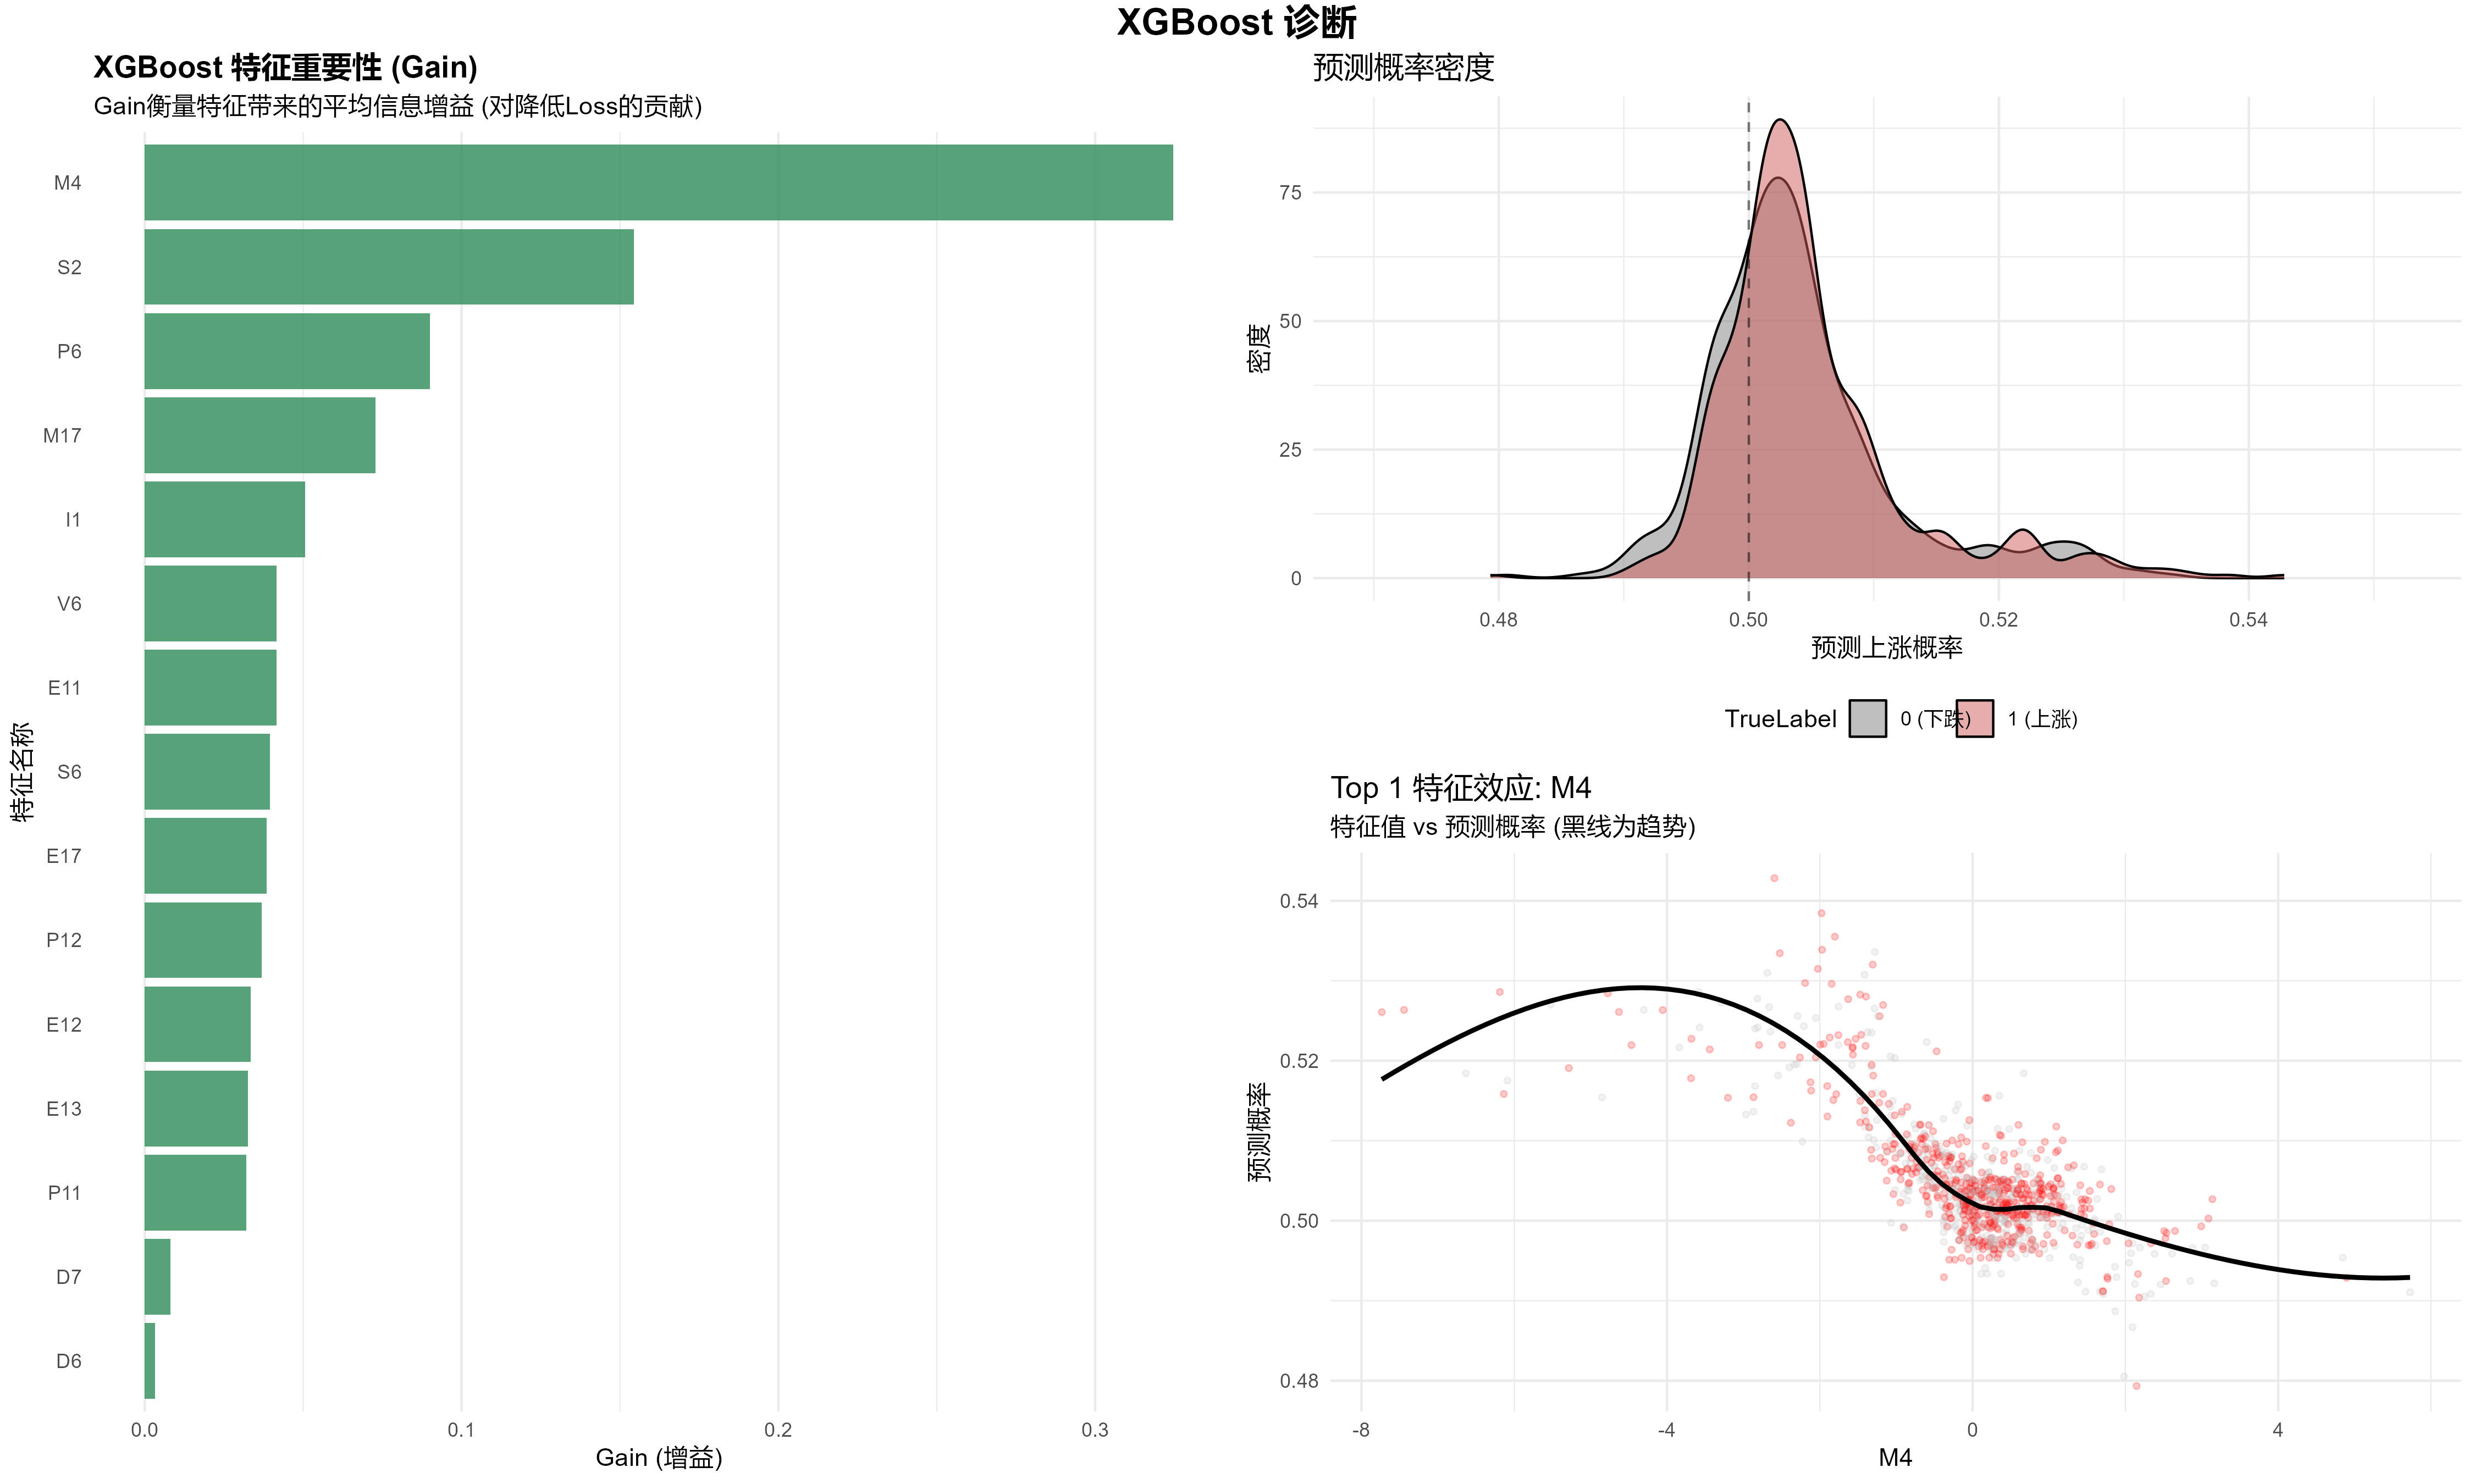
\includegraphics[width=\linewidth]{images/figure2/xgb_analysis_plot (2).png}
    \caption{有Lasso处理}
    \label{fig:right}
  \end{subfigure}
  
  \caption{XGBoost信息增益、预测概率密度分布、M4特征效应} % 大图的总标题
  \label{fig:combined}
\end{figure}
左图中M4因子一枝独秀,Gain 远高于其他特征.筛选出的因子主要为M、P、V因子.右上角的预测概率分布图表明预测概率高度集中在 0.5 附近,并且真实标签之间分布表明了买卖信号依旧不强.右下角的特征效应图张图展示的是最重要的因子 (M4) 的值 与 模型预测的上涨概率之间的关系.图中的黑线这是数据的局部平滑趋势线,波浪形曲线表现M4因子认为说明 M4 与收益率的关系是非线性的,存在复杂的区间效应.然而曲线振幅极小,仅为$\pm 0.5\%$左右.在Lasso筛选变量之后,M4依旧是模型选出的主要因子并且Gain显著上升,说明了M4确实可能是主要解释变量.另外在变量筛选后S2、P6、M17 成为“第二信号源”,这使现在的XGBoost成为由少数几个变量主导方向判断的模型.注意到右上角的预测概率密度相较于没有做Lasso的版本右偏,这可能是因为Lasso将有异号贡献的变量都筛掉了,留下来的变量更偏向于预测上涨.然而即使预测概率产生偏态,模型的分类效果还是没有显著提高.

\clearpage

\section{参考文献}
\bibliography{ref}
\bibliographystyle{plain}
\clearpage


\section{代码实现}
本章包含了之前实现的代码及注释。
\subsection{初步假设检验：寻找支持价值溢价择时策略的证据}
\subsubsection{$\texttt{quant5\_test\_sharpe.r}$}
\begin{minted}{r}
library(PeerPerformance) # 包含Ledoit-Wolf 检验的 sharpeTesting 函数

data_P <- read.csv("train.csv", stringsAsFactors = FALSE)
colindex <- c(58:70)
P_star <- rowMeans(data_P[, colindex], na.rm = TRUE)
P_star <- P_star[-(1:1006)] # 只从第1006条数据开始，因为前面的数据不含有该特征

n_target <- floor(length(P_star) * 0.20)  # 目标数量
sorted_indices <- order(P_star)  # 排序后的索引
label <- rep(FALSE, length(P_star))
label[sorted_indices[1:n_target]] <- TRUE  # 标记Q1组

R_Q1 <- ifelse(label, P_star, 0)
R_P <- P_star

# type = 2 表示使用studentized bootstrap 
# bBoot = 0 表示让函数自动选择最佳块长度
control_params <- list(type = 2, nBoot = 4999, bBoot = 0)

# 执行检验
test_result <- sharpeTesting(R_Q1, R_P, control = control_params)

# 查看 p-value
test_result    
\end{minted}
\subsubsection{$\texttt{quant5\_test\_mdd.r}$}
\begin{minted}{r}
library(tidyverse)

data_P <- read.csv("train.csv", stringsAsFactors = FALSE)

p_colindex <- c(58:70)
P_star_signal <- rowMeans(data_P[, p_colindex], na.rm = TRUE)

R_m_return <- data_P$market_forward_excess_returns

P_star_filtered <- P_star_signal[-(1:1006)]
R_m_filtered <- R_m_return[-(1:1006)]

n_target <- floor(length(P_star_filtered) * 0.20)
sorted_indices <- order(P_star_filtered)
label <- rep(FALSE, length(P_star_filtered))
label[sorted_indices[1:n_target]] <- TRUE

R_Q1 <- ifelse(label, R_m_filtered, 0)
R_P <- R_m_filtered

# 构建净值曲线
V_Q1 <- cumprod(1 + R_Q1)
V_P <- cumprod(1 + R_P)

x_axis <- 1:length(R_P)

# 绘制 V_P
plot(x = x_axis, y = V_P, type = 'l', col = 'blue', 
     main = "策略净值曲线对比",
     xlab = "交易日 (自 date_id 1007 起)", 
     ylab = "净值 (初始 $1)")

# V_Q1
lines(x = x_axis, y = V_Q1, col = 'red')

# 图例
legend("topleft", 
       legend = c("V_P", "V_Q1"), 
       col = c("blue", "red"), 
       lty = 1)    
\end{minted}
\subsection{多因子择时策略下的调仓策略}
\subsubsection{Logistic回归模型}
$\texttt{logistic.r}$
\begin{minted}{r}
# ============================================================
# 模块 1: Logistic 数据处理
# 文件路径: logistic/01_data_processor_logistic.R
# ============================================================

library(dplyr)
library(tidyr)
library(zoo)

process_data_logistic <- function(file_path, config) {
  
  cat("[Data-Logit] 读取数据:", file_path, "...\n")
  if (!file.exists(file_path)) stop("找不到文件")
  raw_data <- read.csv(file_path, stringsAsFactors = FALSE)
  
  if("date_id" %in% names(raw_data)) {
    data_period <- raw_data %>% filter(date_id >= 1006)
  } else {
    data_period <- raw_data[-(1:1006), ]
  }
  
  p_col_names <- names(raw_data)[config$p_cols]
  v_col_names <- names(raw_data)[config$v_cols]
  target_col  <- "market_forward_excess_returns"
  
  # 构造基础数据集 (包含 date_id, target, 和所有 P/V 原始列)
  # 注意：这里我们保留原始列，为了后面做 Imputation
  df_raw <- data_period %>% 
    select(date_id, all_of(target_col), all_of(p_col_names), all_of(v_col_names))
  
  # 构造 Target (0/1)
  df_raw$y <- ifelse(df_raw[[target_col]] >= 0, 1, 0)
  
  # 先切分数据集，再做特征工程
  # ============================================================
  cat("[Data-Logit] 执行时序切分 (Train End:", config$train_end_id, ")...\n")
  
  train_raw <- df_raw %>% filter(date_id <= config$train_end_id)
  test_raw  <- df_raw %>% filter(date_id > config$train_end_id & date_id <= config$test_end_id)
  
  if(nrow(train_raw) == 0) stop("训练集为空")
  
  #  缺失值填补
  # ============================================================
  cat("[Data-Logit] 执行缺失值填补...\n")
  
  impute_cols <- c(p_col_names, v_col_names)
  impute_vals <- sapply(train_raw[impute_cols], median, na.rm = TRUE)
  
  apply_impute <- function(df, vals) {
    for(col in names(vals)) {
      df[[col]][is.na(df[[col]])] <- vals[col]
    }
    return(df)
  }
  
  train_imputed <- apply_impute(train_raw, impute_vals)
  test_imputed  <- apply_impute(test_raw, impute_vals)
  
  # 特征合成
  # ============================================================
  cat("[Data-Logit] 计算合成因子 P_star & V_star...\n")
  
  calc_factors <- function(df) {
    df$P_star <- rowMeans(df[p_col_names])
    df$V_star <- rowMeans(df[v_col_names])
    return(df %>% select(date_id, y, P_star, V_star))
  }
  
  train_factors <- calc_factors(train_imputed)
  test_factors  <- calc_factors(test_imputed)
  
  # 标准化 (Z-Score)
  # ============================================================
  cat("[Data-Logit] 执行标准化\n")
  
  stats <- list(
    p_mean = mean(train_factors$P_star), p_sd = sd(train_factors$P_star),
    v_mean = mean(train_factors$V_star), v_sd = sd(train_factors$V_star)
  )
  
  standardize <- function(x, mu, sigma) { (x - mu) / sigma }
  
  train_factors$P_std <- standardize(train_factors$P_star, stats$p_mean, stats$p_sd)
  train_factors$V_std <- standardize(train_factors$V_star, stats$v_mean, stats$v_sd)
  
  test_factors$P_std  <- standardize(test_factors$P_star, stats$p_mean, stats$p_sd)
  test_factors$V_std  <- standardize(test_factors$V_star, stats$v_mean, stats$v_sd)
  
  # 清理最终包含 NA 的行 (如标准化产生 NaN 或 Target 缺失)
  train_final <- na.omit(train_factors)
  test_final  <- na.omit(test_factors)
  
  cat("[Data-Logit] 处理完成. Train:", nrow(train_final), "| Test:", nrow(test_final), "\n")
  
  return(list(
    train = train_final,
    test = test_final,
    raw_test_set = test_raw, # 保留原始测试集以便后续获取收益率
    stats = stats
  ))
}    
\end{minted}
\subsubsection{SVM模型}
$\texttt{main\_modulized\_handmade.r}$
\begin{minted}{r}
 # ============================================================
# 主程序: SVM
# ============================================================
setwd("C:\\Users\\kagirasu\\works_H\\ml_HULL\\job\\code\\code_section3\\proj_svm")
rm(list = ls())
gc()

library(dplyr)
library(ggplot2)

source("svm_modulized_handmade/algorithm_handmade.R")
source("svm_modulized_handmade/01_data_processor.R")
source("svm_modulized_handmade/02_model_trainer.R")
source("svm_modulized_handmade/03_new.R")

CONFIG <- list(
  # --- 文件路径配置 ---
  input_file  = "data/train.csv",
  output_dir  = "output",

  model_type     = "svm",
  kernel_type    = "rbf",

  missing_thresh = 0.20,    # 缺失率剔除阈值 (20%)
  train_end_id   = 7000,    # 训练集截止 ID
  test_start_id  = 7001,    # 测试集开始 ID
  test_end_id    = 7984,    # 测试集截止 ID
  
  cv_folds       = 2,       # 交叉验证折数
  
  tune_grid      = list(
    # C = c(0.0001, 0.001, 0.01, 0.1, 1.0, 10.0), 
    # C = c(0.1, 1.0, 10.0, 100.0, 1000.0),
    # C = c(10, 100, 1000, 10000, 50000),
    # C = c(0.1:1, 0.2),
    # C = seq(from = 0.01, to = 0.2, by = 0.01),
    # gamma = seq(from = 0.001, to = 0.015, by = 0.003) # RBF 模式下才会用到
     C = 1e-1,
     gamma = 1e-2
  ),
  
  # [调试模式] 固定参数
  # 如果不想每次都跑网格搜索，取消下面这行的注释，就能直接使用最佳参数
 
  fixed_params   = NULL,
  
  target_vol       = 0.20,    # 目标波动率
  max_leverage     = 2,       # 最大杠杆上限
  trend_window     = 60,      # 趋势均线窗口 (MA60)
  prob_roll_window = 60,      # 自适应中枢的回顾窗口 (60天)
  prob_slope       = 10,      # 信号敏感度
  transaction_cost = 0.001
)

if(!dir.exists(CONFIG$output_dir)) dir.create(CONFIG$output_dir)


# ============================================================
# 3. 程序流
# ============================================================

start_time <- Sys.time()
cat(">>> 任务启动时间:", format(start_time, "%Y-%m-%d %H:%M:%S"), "\n")

cat("\n", rep("=", 40), "\n", ">>> 阶段1: 数据预处理\n", rep("=", 40), "\n", sep="")
tryCatch({
  data_bundle <- process_data(CONFIG$input_file, CONFIG)
}, error = function(e) {
  stop("数据处理阶段出错: ", e$message)
})

cat("\n", rep("=", 40), "\n", ">>> 阶段2: 模型训练\n", rep("=", 40), "\n", sep="")
tryCatch({
  model_bundle <- train_model_entry(data_bundle, CONFIG)
}, error = function(e) {
  stop("模型训练阶段出错: ", e$message)
})

cat("\n", rep("=", 40), "\n", ">>> 阶段3: 策略回测\n", rep("=", 40), "\n", sep="")
tryCatch({
  backtest_results <- run_strategy_backtest(data_bundle, model_bundle, CONFIG)
}, error = function(e) {
  stop("策略回测阶段出错: ", e$message)
})

# ============================================================
# 4. 结束摘要
# ============================================================
end_time <- Sys.time()
duration <- round(difftime(end_time, start_time, units = "mins"), 2)

cat("\n", rep("=", 40), "\n", ">>> 所有任务执行完毕！\n", rep("=", 40), "\n", sep="")
cat("  - 总耗时:", duration, "分钟\n")
cat("  - 输出目录:", CONFIG$output_dir, "\n")
cat("  - 最终夏普比率:", round(backtest_results$metrics$Strategy[2], 4), "\n")
cat("  - 结果图表: backtest_equity_curve.png\n")   
\end{minted}
$\texttt{01\_data\_processor.r}$
\begin{minted}{r}
# ============================================================
# 模块 1: SVM数据预处理
# ============================================================

library(dplyr)
library(tidyr)
library(zoo)

#' 处理数据的主函数
process_data <- function(file_path, config) {
  
  cat("[Data] 正在读取数据:", file_path, "...\n")

  if (!file.exists(file_path)) stop("错误: 找不到数据文件 -> ", file_path)
  raw_data <- read.csv(file_path, stringsAsFactors = FALSE)
  
  target_col_raw <- "market_forward_excess_returns"
  id_cols <- c("date_id", "forward_returns", "risk_free_rate")
  potential_features <- setdiff(names(raw_data), c(target_col_raw, id_cols))
  
  # 数据切片: 仅处理有效时间段
  data_period <- raw_data %>%
    filter(date_id >= 1006) %>%
    arrange(date_id)
  
  # ------------------------------------------------------------
  # 特征筛选防泄露
  # 必须仅基于训练集 (date_id <= train_end_id) 来决定删除哪些列
  # ------------------------------------------------------------
  cat("[Data] 正在基于训练集统计特征缺失率...\n")
  
  train_subset_for_stats <- data_period %>% 
    filter(date_id <= config$train_end_id)
  
  if(nrow(train_subset_for_stats) == 0) stop("错误: 训练集为空，请检查配置！")
  
  missing_ratio <- colMeans(is.na(train_subset_for_stats[potential_features]))
  
  # 剔除特征
  threshold <- config$missing_thresh
  cols_to_drop <- names(missing_ratio[missing_ratio > threshold])
  final_feature_cols <- setdiff(potential_features, cols_to_drop)
  
  cat("[Data] 特征筛选报告:\n")
  cat("  - 初始特征数:", length(potential_features), "\n")
  cat("  - 剔除特征数:", length(cols_to_drop), "(基于训练集)\n")
  cat("  - 最终保留特征:", length(final_feature_cols), "\n")
  
  # ------------------------------------------------------------
  # 样本清洗与填充
  data_pruned <- data_period %>% 
    select(date_id, all_of(target_col_raw), all_of(final_feature_cols))
  
  data_filled <- na.locf(data_pruned, na.rm = FALSE)
  
  complete_data <- na.omit(data_filled)
  
  complete_data$y_target <- factor(
    ifelse(complete_data[[target_col_raw]] >= 0, 1, 0), 
    levels = c(0, 1)
  )
  
  train_set <- complete_data %>% filter(date_id <= config$train_end_id)
  test_set  <- complete_data %>% filter(date_id >= config$test_start_id & date_id <= config$test_end_id)
  
  # ------------------------------------------------------------
  # Z-Score 标准化
  # ------------------------------------------------------------
  cat("[Data] 执行 Z-Score 标准化\n")
  scaler_params <- algo_zscore_fit(train_set[final_feature_cols])
  
  X_train_mat <- algo_zscore_transform(train_set[final_feature_cols], scaler_params)
  X_test_mat  <- algo_zscore_transform(test_set[final_feature_cols], scaler_params)
  
  return(list(
    X_train = as.data.frame(X_train_mat),
    y_train = train_set$y_target,
    X_test  = as.data.frame(X_test_mat),
    y_test  = test_set$y_target,
    raw_train_set = train_set,
    raw_test_set  = test_set,
    scaling_params = scaler_params
  ))
}
\end{minted}
$\texttt{02\_model\_trainer.r}$
\begin{minted}{r}
# ============================================================
# 模块 2: 模型训练器
# ============================================================

library(dplyr)

# F1
calc_f1 <- function(scores, y_true) {
  y_pred <- ifelse(scores >= 0, 1, 0)
  y_true <- as.numeric(as.character(y_true))
  tp <- sum(y_pred == 1 & y_true == 1)
  fp <- sum(y_pred == 1 & y_true == 0)
  fn <- sum(y_pred == 0 & y_true == 1)
  precision <- if ((tp + fp) == 0) 0 else tp / (tp + fp)
  recall    <- if ((tp + fn) == 0) 0 else tp / (tp + fn)
  if ((precision + recall) == 0) 0 else 2 * precision * recall / (precision + recall)
}

train_model_entry <- function(data_bundle, config) {
  model_type <- if(is.null(config$model_type)) "svm" else config$model_type
  if (model_type == "svm") return(train_svm_model(data_bundle, config))
  else stop("不支持非SVM模型")
}

train_svm_model <- function(data_bundle, config) {
  
  X_train <- as.matrix(data_bundle$X_train)
  y_train <- data_bundle$y_train
  X_test  <- as.matrix(data_bundle$X_test)
  
  # 获取核函数类型，默认为 Linear
  k_type <- if(is.null(config$kernel_type)) "linear" else config$kernel_type
  cat(sprintf("[Model] 初始化 SVM 训练流程, Kernel = %s\n", toupper(k_type)))
  
  # ============================================================
  # 网格搜索
  # ============================================================
  
  if (k_type == "linear") {
    tune_grid <- expand.grid(C = config$tune_grid$C, gamma = 0) # gamma 0 占位
    cat("[Model] 线性核模式: 仅搜索参数 C\n")
  } else {
    tune_grid <- expand.grid(C = config$tune_grid$C, gamma = config$tune_grid$gamma)
    cat("[Model] RBF核模式: 搜索参数 C 和 Gamma\n")
  }
  
  best_score <- -1
  best_params <- list(C = 0.1, gamma = 0.01) # 默认
  
  k_folds <- config$cv_folds
  folds <- cut(seq(1, nrow(X_train)), breaks = k_folds, labels = FALSE)
  
  for(i in 1:nrow(tune_grid)) {
    curr_C <- tune_grid$C[i]
    curr_g <- tune_grid$gamma[i]
    
    if (k_type == "linear") {
      cat(sprintf("  > Grid Search [%d/%d] C=%.4f ... ", i, nrow(tune_grid), curr_C))
    } else {
      cat(sprintf("  > Grid Search [%d/%d] C=%.4f Gamma=%.4f ... ", i, nrow(tune_grid), curr_C, curr_g))
    }
    
    fold_scores <- numeric(k_folds)
    
    for(k in 1:k_folds) {
      idx_val <- which(folds == k)
      idx_tr  <- which(folds != k)
      
      # 训练 Fold 模型
      tm_model <- algo_svm_train_smo(
        X_train[idx_tr, ], y_train[idx_tr], 
        C = curr_C, gamma = curr_g, 
        kernel_type = k_type,
        max_iter = 5000 # 搜索时加速
      )
      
      val_s <- algo_svm_predict_score(tm_model, X_train[idx_val, ])
      fold_scores[k] <- calc_f1(val_s, y_train[idx_val])
    }
    
    avg_score <- mean(fold_scores, na.rm=TRUE)
    cat(sprintf("F1=%.4f\n", avg_score))
    
    if(avg_score > best_score) {
      best_score <- avg_score
      best_params <- list(C = curr_C, gamma = curr_g)
    }
  }
  
gamma_str <- if (!is.null(best_params$gamma)) sprintf(", Gamma=%.4f", best_params$gamma) else ""

cat(sprintf("[Model] 最佳参数找到: C=%.4f%s\n", best_params$C, gamma_str))
  
  # ============================================================
  # 2. 内部CV拟合Platt Scaling
  # ============================================================
  cat("[Model] 执行 Internal CV 以校准概率...\n")
  
  n_calib_folds <- 3
  folds_calib <- cut(seq(1, nrow(X_train)), breaks = n_calib_folds, labels = FALSE)
  cv_scores <- numeric(nrow(X_train))
  
  for(k in 1:n_calib_folds) {
    idx_val <- which(folds_calib == k)
    idx_tr  <- which(folds_calib != k)
    
    sub_model <- algo_svm_train_smo(
      X_train[idx_tr, ], y_train[idx_tr], 
      C = best_params$C, gamma = best_params$gamma,
      kernel_type = k_type,
      max_iter = 100 
    )
    cv_scores[idx_val] <- algo_svm_predict_score(sub_model, X_train[idx_val, ])
  }
  
  platt_params <- algo_platt_fit(cv_scores, as.numeric(as.character(y_train)))
  
  # ============================================================
  # 3. 训练最终模型
  # ============================================================
  cat("[Model] 使用最佳参数训练全量模型...\n")
  
  final_model <- algo_svm_train_smo(
    X_train, y_train, 
    C = best_params$C, gamma = best_params$gamma,
    kernel_type = k_type,
    max_iter = 1000 # 保证收敛
  )
  
  # 统计 SV
  n_sv <- length(final_model$sv_indices)
  sv_ratio <- n_sv / nrow(X_train)
  cat(sprintf("[Model-Stats] SV 占比: %.2f%% (Kernel: %s)\n", sv_ratio * 100, k_type))
  
  test_scores <- algo_svm_predict_score(final_model, X_test)
  saveRDS(final_model, file.path(config$output_dir, "svm_best_model.rds"))
  
  return(list(
    model = final_model,
    test_scores = test_scores,
    platt_params = platt_params,
    best_params = best_params,
    sv_ratio = sv_ratio
  ))
}    
\end{minted}
$\texttt{03\_new.r}$
\begin{minted}{r}
# ============================================================
# 模块 3: 策略回测 (添加费率因素)
# ============================================================

library(zoo)
library(dplyr)
library(ggplot2)

run_strategy_backtest <- function(data_bundle, model_bundle, config) {
  
  cat("[Strategy] 启动策略回测...\n")
  
  p_target_vol   <- if(is.null(config$target_vol)) 0.15 else config$target_vol
  p_max_leverage <- if(is.null(config$max_leverage)) 2.0 else config$max_leverage
  p_trend_window <- if(is.null(config$trend_window)) 60 else config$trend_window
  p_roll_window  <- if(is.null(config$prob_roll_window)) 60 else config$prob_roll_window
  p_prob_slope   <- if(is.null(config$prob_slope)) 10 else config$prob_slope
  p_trans_cost   <- if(is.null(config$transaction_cost)) 0.001 else config$transaction_cost 
  
  cat(sprintf("  - 参数: Vol=%.2f Lev=%.1f Cost=%.4f\n", 
              p_target_vol, p_max_leverage, p_trans_cost))
  
  # 概率校准
  test_set <- data_bundle$raw_test_set
  test_scores <- as.numeric(model_bundle$test_scores)
  
  if (length(test_scores) == 0) stop("错误: 无预测得分")
  if (is.null(model_bundle$platt_params)) stop("错误: 缺少 Platt 参数")
  
  platt_params <- model_bundle$platt_params
  test_probs <- algo_platt_predict(test_scores, platt_params)
  test_set$pred_prob <- test_probs
  
  vol_zoo <- rollapply(test_set$market_forward_excess_returns, 
                       width = 20, FUN = sd, fill = NA, align = "right") * sqrt(252)
  current_vol <- as.numeric(vol_zoo)
  current_vol[is.na(current_vol) | current_vol <= 0] <- p_target_vol 
  
  price_index <- cumprod(1 + test_set$market_forward_excess_returns)
  ma_trend <- rollapply(price_index, width = p_trend_window, FUN = mean, fill = NA, align = "right")
  ma_trend[is.na(ma_trend)] <- price_index[is.na(ma_trend)]
  is_bull <- ifelse(price_index > ma_trend, 1, 0)
  
  # 仓位计算
  rolling_median <- rollapply(test_set$pred_prob, width = p_roll_window, 
                              FUN = median, fill = NA, align = "right")
  test_set$adaptive_center <- dplyr::lag(rolling_median, n = 1)
  
  default_center <- median(test_set$pred_prob, na.rm = TRUE)
  test_set$adaptive_center[is.na(test_set$adaptive_center)] <- default_center
  
  signal_score <- 0.5 + (test_set$pred_prob - test_set$adaptive_center) * p_prob_slope
  base_pos <- pmax(0.2, pmin(1.5, signal_score))
  
  vol_scaler <- p_target_vol / current_vol
  trend_mult <- ifelse(is_bull == 1, 1.0, 0.6)
  
  raw_pos <- base_pos * vol_scaler * trend_mult
  test_set$position <- pmin(raw_pos, p_max_leverage)
  test_set$position[is.na(test_set$position)] <- 0
  
  cat("  - 平均持仓:", round(mean(test_set$position), 2), "\n")
  
  # 4. 绩效统计 (含交易成本)
  # ============================================================
  pos_change <- diff(c(0, test_set$position))
  turnover_cost <- abs(pos_change) * p_trans_cost
  
  # 净收益 = (持仓 * 市场收益) - 成本
  test_set$gross_return <- test_set$position * test_set$market_forward_excess_returns
  test_set$strategy_return <- test_set$gross_return - turnover_cost
  
  cat(sprintf("  - [Cost] 总交易成本损耗: %.2f%%\n", sum(turnover_cost)*100))
  
  calc_metrics <- function(ret) {
    ret <- as.numeric(ret)
    total <- prod(1 + ret, na.rm=TRUE) - 1
    ann <- (1 + total)^(252/length(ret)) - 1
    vol <- sd(ret, na.rm=TRUE) * sqrt(252)
    sharpe <- if(vol==0) 0 else ann/vol
    dd <- min((cumprod(1+ret)/cummax(cumprod(1+ret)))-1, na.rm=TRUE)
    return(c(Ann_Return=ann, Sharpe=sharpe, Max_DD=dd))
  }
  
  res_strat <- calc_metrics(test_set$strategy_return)
  res_mkt   <- calc_metrics(test_set$market_forward_excess_returns)
  
  metrics_df <- data.frame(Metric=names(res_strat), Market=round(res_mkt,4), Strategy=round(res_strat,4))
  cat("\n----------- 回测绩效报告 (费后) -----------\n")
  print(metrics_df)
  
  write.csv(metrics_df, file.path(config$output_dir, "performance_metrics.csv"), row.names = FALSE)
  
  plot_df <- data.frame(
    Time = 1:nrow(test_set),
    Market = cumprod(1 + test_set$market_forward_excess_returns),
    Strategy = cumprod(1 + test_set$strategy_return)
  )
  if("date_id" %in% names(test_set)) plot_df$Time <- test_set$date_id
  
  p <- ggplot(plot_df, aes(x = Time)) +
    geom_line(aes(y = Market, color = "Market"), alpha = 0.6) +
    geom_line(aes(y = Strategy, color = "SVM Strategy (Net)"), linewidth = 1) +
    scale_color_manual(values = c("Market"="grey", "SVM Strategy (Net)"="red")) +
    labs(title = "SVM Strategy Performance (Net of Cost)",
         subtitle = paste("Sharpe:", round(res_strat['Sharpe'], 2), 
                          "| Cost:", p_trans_cost*10000, "bps")) +
    theme_minimal()
  
  ggsave(file.path(config$output_dir, "equity_curve.png"), p, width=8, height=5)
  
  return(list(results_df=test_set, metrics=metrics_df, plot=p))
}
\end{minted}
$\texttt{algorithm\_handmade.r}$，这里也包含了后面几个模型的算法。
\begin{minted}{r}
# ------------------------------------------------------------
#  Z-Score 标准化算法
# ------------------------------------------------------------
#' @param X 特征矩阵或数据框
#' @return list(mean, sd)
algo_zscore_fit <- function(X) {
  # 强制转换为矩阵
  X_mat <- as.matrix(X)
  
  # 1. 计算列均值
  mu <- colMeans(X_mat, na.rm = TRUE)
  
  # 2. 计算列标准差 (使用apply循环)
  sigma <- apply(X_mat, 2, sd, na.rm = TRUE)
  
  sigma[sigma == 0] <- 1
  
  return(list(mean = mu, sd = sigma))
}

#' [算法] 应用标准化转换
#' 数学原理: z_i = (x_i - mu) / sigma
#' @param X 需要转换的数据
#' @param params algo_zscore_fit 返回的参数列表
#' @return 标准化后的矩阵
algo_zscore_transform <- function(X, params) {
  X_mat <- as.matrix(X)
  mu <- params$mean
  sigma <- params$sd
  
  if (ncol(X_mat) != length(mu)) {
    stop(paste("维度不匹配: 数据列数", ncol(X_mat), "!= 参数列数", length(mu)))
  }
  X_scaled <- t((t(X_mat) - mu) / sigma)
  
  return(X_scaled)
}

#' [算法] 线性核矩阵计算
algo_kernel_linear <- function(X1, X2) {
  tcrossprod(as.matrix(X1), as.matrix(X2))
}

#' [算法] RBF 核矩阵计算
#' @param X1 矩阵 n x d
#' @param X2 矩阵 m x d
#' @param gamma 核参数
algo_kernel_rbf <- function(X1, X2, gamma) {
  X1 <- as.matrix(X1)
  X2 <- as.matrix(X2)
  
  n <- nrow(X1)
  m <- nrow(X2)
  
  sq_norm1 <- rowSums(X1^2)
  sq_norm2 <- rowSums(X2^2)
  dot_prod <- tcrossprod(X1, X2)
  
  dist_sq <- outer(sq_norm1, sq_norm2, "+") - 2 * dot_prod
  
  K <- exp(-gamma * dist_sq)
  return(K)
}

#' [算法]SMO训练SVM
#' @param kernel_type "linear" 或 "rbf"
#' @param gamma RBF核需要此参数，Linear核忽略
algo_svm_train_smo <- function(X, y, C, kernel_type="linear", gamma=NULL, max_iter=100, tol=1e-3) {
  
  X_mat <- as.matrix(X)
  y_vec <- as.numeric(as.character(y)) 
  if (all(y_vec %in% c(0, 1))) y_vec[y_vec == 0] <- -1
  
  n_samples <- nrow(X_mat)
  alphas <- numeric(n_samples)
  b <- 0
  
  # --------------------------------------------------------
  # 根据 kernel_type 预计算核矩阵 K
  # --------------------------------------------------------
  if (kernel_type == "rbf") {
    if(is.null(gamma)) stop("RBF核必须提供 gamma 参数")
    K <- algo_kernel_rbf(X_mat, X_mat, gamma)
  } else if (kernel_type == "linear") {
    K <- algo_kernel_linear(X_mat, X_mat)
  } else {
    stop(paste("未知的 kernel_type:", kernel_type))
  }
  
  passes <- 0 
  iter_count <- 0
  
  cat(sprintf("  [SMO] Start: Kernel=%s, C=%.4f, Samples=%d\n", kernel_type, C, n_samples))
  
  while (passes < 10 && iter_count < max_iter) {
    num_changed_alphas <- 0
    iter_count <- iter_count + 1
    
    for (i in 1:n_samples) {
      f_xi <- sum(alphas * y_vec * K[, i]) + b
      E_i <- f_xi - y_vec[i]
      
      if ((y_vec[i] * E_i < -tol && alphas[i] < C) || 
          (y_vec[i] * E_i > tol && alphas[i] > 0)) {
        
        j <- sample(setdiff(1:n_samples, i), 1)
        f_xj <- sum(alphas * y_vec * K[, j]) + b
        E_j <- f_xj - y_vec[j]
        
        alpha_i_old <- alphas[i]
        alpha_j_old <- alphas[j]
        
        if (y_vec[i] != y_vec[j]) {
          L <- max(0, alpha_j_old - alpha_i_old)
          H <- min(C, C + alpha_j_old - alpha_i_old)
        } else {
          L <- max(0, alpha_i_old + alpha_j_old - C)
          H <- min(C, alpha_i_old + alpha_j_old)
        }
        
        if (L == H) next
        
        eta <- 2 * K[i, j] - K[i, i] - K[j, j]
        if (eta >= 0) next
        
        alphas[j] <- alphas[j] - (y_vec[j] * (E_i - E_j)) / eta
        
        if (alphas[j] > H) alphas[j] <- H
        if (alphas[j] < L) alphas[j] <- L
        
        if (abs(alphas[j] - alpha_j_old) < 1e-5) next
        
        alphas[i] <- alphas[i] + y_vec[i] * y_vec[j] * (alpha_j_old - alphas[j])
        
        b1 <- b - E_i - y_vec[i] * (alphas[i] - alpha_i_old) * K[i, i] - 
              y_vec[j] * (alphas[j] - alpha_j_old) * K[i, j]
        b2 <- b - E_j - y_vec[i] * (alphas[i] - alpha_i_old) * K[i, j] - 
              y_vec[j] * (alphas[j] - alpha_j_old) * K[j, j]
        
        if (0 < alphas[i] && alphas[i] < C) { b <- b1 } 
        else if (0 < alphas[j] && alphas[j] < C) { b <- b2 } 
        else { b <- (b1 + b2) / 2 }
        
        num_changed_alphas <- num_changed_alphas + 1
      }
    }
    
    if (num_changed_alphas == 0) passes <- passes + 1 else passes <- 0
  }
  
  sv_idx <- which(alphas > 1e-5)
  
  return(list(
    alphas = alphas[sv_idx],
    sv_indices = sv_idx,
    sv_X = X_mat[sv_idx, , drop=FALSE],
    sv_y = y_vec[sv_idx],
    b = b,
    gamma = gamma,
    kernel = kernel_type
  ))
}

#' [算法]SVM预测
#' 根据模型中的 kernel 类型自动选择计算方式
algo_svm_predict_score <- function(model, X_new) {
  X_new <- as.matrix(X_new)
  
  if (model$kernel == "rbf") {
    K_new <- algo_kernel_rbf(X_new, model$sv_X, model$gamma)
  } else if (model$kernel == "linear") {
    K_new <- algo_kernel_linear(X_new, model$sv_X)
  } else {
    stop("模型包含未知的 kernel 类型")
  }
  
  weights <- model$alphas * model$sv_y
  decision_values <- (K_new %*% weights) + model$b
  
  return(as.vector(decision_values))
}

########### 还没有输出概率 ###############

# ============================================================
# 3. 概率校准
# ============================================================

#' [算法] 使用牛顿法求解 Sigmoid 参数
#' @param scores SVM 输出的决策值向量 f(x)
#' @param y 真实标签向量 (0 或 1)
#' @return list(A, B)
algo_platt_fit <- function(scores, y, max_iter = 100, tol = 1e-5) {
  # Platt 对标签进行平滑处理以避免过拟合
  prior0 <- sum(y == 0)
  prior1 <- sum(y == 1)
  
  hi_target <- (prior1 + 1.0) / (prior1 + 2.0)
  lo_target <- 1 / (prior0 + 2.0)
  
  t <- ifelse(y == 1, hi_target, lo_target)
  
  A <- 0.0
  B <- log((prior0 + 1.0) / (prior1 + 1.0))
  
  # 牛顿法迭代
  for (it in 1:max_iter) {
    f_ap_b <- scores * A + B
    
    p <- ifelse(f_ap_b >= 0, 
                exp(-f_ap_b) / (1.0 + exp(-f_ap_b)), 
                1.0 / (1.0 + exp(f_ap_b)))
    
    d <- p - t
    h <- p * (1.0 - p)
    sigma <- 1e-12 # 防止除零
    h <- pmax(h, sigma)
    
    grad_A <- sum(scores * d)
    grad_B <- sum(d)
    hess_AA <- sum(scores * scores * h)
    hess_BB <- sum(h)
    hess_AB <- sum(scores * h)
    
    det <- hess_AA * hess_BB - hess_AB * hess_AB
    
    if (abs(det) < 1e-12) break
    
    dA <- (hess_BB * grad_A - hess_AB * grad_B) / det
    dB <- (hess_AA * grad_B - hess_AB * grad_A) / det
    
    old_A <- A
    old_B <- B
    
    A <- A + dA
    B <- B + dB
    
    if (abs(A - old_A) < tol && abs(B - old_B) < tol) break
  }
  
  return(list(A = A, B = B))
}

#' [算法] Sigmoid 预测
#' @param scores 决策值
#' @param params Platt Scaling 参数 (A, B)
#' @return 概率值
algo_platt_predict <- function(scores, params) {
  f_ap_b <- scores * params$A + params$B
  
  # Sigmoid 函数
  p <- ifelse(f_ap_b >= 0, 
              exp(-f_ap_b) / (1.0 + exp(-f_ap_b)), 
              1.0 / (1.0 + exp(f_ap_b)))
  return(p)
}

# ============================================================
# 4. Logistic 回归核心算法
# ============================================================

#' [算法] Sigmoid 函数
algo_sigmoid <- function(z) {
  1 / (1 + exp(-z))
}

#' [算法] Logistic 回归训练 (梯度下降法)
#' @param X 特征矩阵
#' @param y 标签 (0/1)
#' @param learning_rate 学习率
#' @param lambda 正则化系数 (L2)
#' @param max_iter 最大迭代次数
algo_logistic_train_gd <- function(X, y, learning_rate = 0.01, lambda = 0.1, max_iter = 1000) {
  
  X_mat <- as.matrix(X)
  y_vec <- as.numeric(as.character(y))
  
  m <- nrow(X_mat)
  n <- ncol(X_mat)
  
  weights <- rep(0, n)
  bias <- 0
  for (i in 1:max_iter) {
    z <- (X_mat %*% weights) + bias
    p <- algo_sigmoid(z)
    error <- p - y_vec
    dw <- (1/m) * (t(X_mat) %*% error) + (lambda/m) * weights
    db <- (1/m) * sum(error)
    
    weights <- weights - learning_rate * dw
    bias <- bias - learning_rate * db
  }
  
  return(list(
    weights = weights,
    bias = bias,
    model_type = "logistic"
  ))
}

#' [算法] Logistic 预测
#' @return list(scores, probs)
algo_logistic_predict <- function(model, X) {
  X_mat <- as.matrix(X)
  
  z <- (X_mat %*% model$weights) + model$bias
  
  probs <- algo_sigmoid(z)
  
  return(list(scores = as.vector(z), probs = as.vector(probs)))
}


# ============================================================
# 5. RF
# 组件: CART 决策树, Gini 纯度, Bootstrap, Bagging
# ============================================================

# ------------------------------------------------------------
# A. 基础函数
# ------------------------------------------------------------

#' [算法] 计算 Gini 不纯度
#' 公式: 1 - sum(p_i^2)
algo_cart_gini <- function(y) {
  if (length(y) == 0) return(0)
  props <- prop.table(table(y))
  1 - sum(props^2)
}

#' [算法] 寻找最佳切分点
#' @param X 特征矩阵
#' @param y 标签向量
#' @param mtry 随机采样的特征数量
#' @return list(feature_idx, threshold, gain) 或 NULL
algo_cart_find_split <- function(X, y, mtry) {
  
  n_samples <- nrow(X)
  n_features <- ncol(X)
  current_gini <- algo_cart_gini(y)
  
  best_gain <- 0
  best_split <- NULL
  
  # 随机选择 mtry 个特征的索引
  feat_indices <- sample(1:n_features, min(mtry, n_features))
  
  # 遍历选中的特征
  for (feat_idx in feat_indices) {
    x_col <- X[, feat_idx]
    
    if (length(unique(x_col)) <= 1) next
    
    ord <- order(x_col)
    x_sorted <- x_col[ord]
    y_sorted <- y[ord]

    is_change <- c(diff(x_sorted) != 0, FALSE) # 最后一位补FALSE
    if (!any(is_change)) next
    
    split_indices <- which(is_change)
    
    # ------------------------------------------------------
    # 计算所有切分点的 Gini
    # ------------------------------------------------------
    y_numeric <- as.numeric(y_sorted) - 1
    
    n_left <- split_indices
    n_right <- n_samples - n_left
    cum_sum <- cumsum(y_numeric)
    p1_left_count <- cum_sum[split_indices]
    total_p1 <- sum(y_numeric)
    p1_right_count <- total_p1 - p1_left_count
    
    gini_left <- 1 - ( (p1_left_count/n_left)^2 + ((n_left-p1_left_count)/n_left)^2 )
    gini_right <- 1 - ( (p1_right_count/n_right)^2 + ((n_right-p1_right_count)/n_right)^2 )
    
    gini_split <- (n_left / n_samples) * gini_left + (n_right / n_samples) * gini_right
    
    gains <- current_gini - gini_split
    
    max_g_idx <- which.max(gains)
    max_g <- gains[max_g_idx]
    
    if (max_g > best_gain) {
      best_gain <- max_g
      idx_in_sorted <- split_indices[max_g_idx]
      threshold <- (x_sorted[idx_in_sorted] + x_sorted[idx_in_sorted+1]) / 2
      
      best_split <- list(
        feature_idx = feat_idx,
        threshold = threshold,
        gain = best_gain
      )
    }
  }
  
  return(best_split)
}

# ------------------------------------------------------------
# B. 树构建函数
# ------------------------------------------------------------

#' [算法] 递归构建决策树
#' @param current_depth 当前深度
#' @param max_depth 最大深度限制
#' @param min_node_size 叶节点最小样本数
algo_cart_build_tree <- function(X, y, current_depth, max_depth, min_node_size, mtry) {
  
  # 1. 检查停止条件
  if (current_depth >= max_depth || 
      nrow(X) < min_node_size || 
      length(unique(y)) == 1) {
    
    # 返回叶节点
    prob_1 <- mean(as.numeric(y) == 1)
    return(list(type = "leaf", prob = prob_1, samples = nrow(X)))
  }
  
  split <- algo_cart_find_split(X, y, mtry)
  
  if (is.null(split)) {
    prob_1 <- mean(as.numeric(y) == 1)
    return(list(type = "leaf", prob = prob_1, samples = nrow(X)))
  }

  feat_col <- X[, split$feature_idx]
  left_mask <- feat_col <= split$threshold
  
  X_left <- X[left_mask, , drop=FALSE]
  y_left <- y[left_mask]
  X_right <- X[!left_mask, , drop=FALSE]
  y_right <- y[!left_mask]

  left_node <- algo_cart_build_tree(X_left, y_left, current_depth + 1, max_depth, min_node_size, mtry)
  right_node <- algo_cart_build_tree(X_right, y_right, current_depth + 1, max_depth, min_node_size, mtry)
  
  return(list(
    type = "split",
    feature_idx = split$feature_idx,
    threshold = split$threshold,
    left = left_node,
    right = right_node,
    gain = split$gain
  ))
}

# ------------------------------------------------------------
# C. 预测函数
# ------------------------------------------------------------

#' [算法] 单样本预测
algo_cart_predict_sample <- function(tree, sample_vec) {
  node <- tree
  while (node$type == "split") {
    val <- sample_vec[node$feature_idx]
    if (val <= node$threshold) {
      node <- node$left
    } else {
      node <- node$right
    }
  }
  return(node$prob)
}

#' [算法] 整树预测 (批量)
algo_cart_predict_batch <- function(tree, X) {
  probs <- apply(X, 1, function(row) algo_cart_predict_sample(tree, row))
  return(probs)
}

# ------------------------------------------------------------
# D. Bagging
# ------------------------------------------------------------

#' [算法] RF训练
algo_rf_train_custom <- function(X, y, ntree, mtry, max_depth = 5, min_node_size = 10) {
  
  n_samples <- nrow(X)
  forest <- list()
  
  # 循环建立 ntree 棵树
  for (i in 1:ntree) {
    # Bootstrap
    boot_idx <- sample(1:n_samples, n_samples, replace = TRUE)
    X_boot <- X[boot_idx, , drop=FALSE]
    y_boot <- y[boot_idx]
    
    # 构建树
    tree <- algo_cart_build_tree(X_boot, y_boot, 
                                 current_depth = 0, 
                                 max_depth = max_depth, 
                                 min_node_size = min_node_size, 
                                 mtry = mtry)
    
    forest[[i]] <- tree
  }
  
  return(forest)
}
\end{minted}
\subsubsection{RF模型}
包含了主程序$\texttt{main\_rf.r}$,$\texttt{01\_data\_processor\_rf.r}$处理数据，$\texttt{02\_model\_trainer\_rf\_handmade.r}$完成算法部分并训练模型，$\texttt{03\_strategy\_engine\_rf.r}$回测。

$\texttt{main\_rf.r}$
\begin{minted}{r}
# ============================================================
# 主程序: RF主控
# ============================================================

# ============================================================
rm(list = ls())
gc()
setwd("C:/Users/kagirasu/works_H/ml_HULL/job/code/code_section3")

library(dplyr)
library(zoo)
library(ggplot2)

source("proj_svm/svm_modulized_handmade/algorithm_handmade.r")
source("RF/01_data_processor_rf.R")
source("RF/02_model_trainer_rf_handmade.R")
source("RF/03_strategy_engine_rf.R")

CONFIG <- list(
  input_file      = "proj_svm/data/train.csv",
  output_dir      = "output_rf_fixed",

  missing_thresh  = 0.20,
  train_end_id    = 7000,
  test_start_id   = 7001,
  test_end_id     = 7984,
  na_handling     = "zero",
  
  rf_params       = list(
    ntree      = 500,     # 树的数量
    mtry       = "sqrt",  # 每次分裂随机选取的特征数
    nodesize   = 5,       # 叶节点最小样本数
    max_depth  = 10,      # 限制深度防止过拟合
    importance = TRUE     # 开启特征重要性计算
  ),
  
  target_vol       = 0.2,     # 目标波动率
  max_leverage     = 2.0,     # 最大杠杆
  trend_window     = 60,      # 趋势均线窗口
  prob_roll_window = 60,      # 自适应中枢窗口
  prob_slope       = 8,       # 信号敏感度
  transaction_cost = 0.001    # 交易费用
)

if(!dir.exists(CONFIG$output_dir)) dir.create(CONFIG$output_dir)

# ============================================================
# 程序流
# ============================================================

start_time <- Sys.time()
cat(">>> [RF Project] 任务启动时间:", format(start_time, "%Y-%m-%d %H:%M:%S"), "\n")

cat("\n", rep("=", 40), "\n", ">>> 阶段 I: 数据预处理\n", rep("=", 40), "\n", sep="")
tryCatch({
  data_bundle <- process_data_rf(CONFIG$input_file, CONFIG)
}, error = function(e) {
  stop("数据处理阶段出错: ", e$message)
})

cat("\n", rep("=", 40), "\n", ">>> 阶段 II: 随机森林训练\n", rep("=", 40), "\n", sep="")
tryCatch({
  model_bundle <- train_rf_model(data_bundle, CONFIG)
}, error = function(e) {
  stop("模型训练阶段出错: ", e$message)
})

cat("\n", rep("=", 40), "\n", ">>> 阶段 III: 策略回测\n", rep("=", 40), "\n", sep="")
tryCatch({
  backtest_results <- run_strategy_backtest_rf(data_bundle, model_bundle, CONFIG)
}, error = function(e) {
  stop("策略回测阶段出错: ", e$message)
})

# ============================================================
# 结束摘要
# ============================================================
end_time <- Sys.time()
duration <- round(difftime(end_time, start_time, units = "mins"), 2)

cat("\n", rep("=", 40), "\n", ">>> [RF Project] 所有任务执行完毕！\n", rep("=", 40), "\n", sep="")
cat("  - 总耗时:", duration, "分钟\n")
cat("  - 输出目录:", CONFIG$output_dir, "\n")
if(!is.null(backtest_results$metrics)) {
  cat("  - 最终费后夏普比率:", backtest_results$metrics[backtest_results$metrics$Metric=="Sharpe", "Strategy"], "\n")
}
cat("  - 结果文件已保存。\n")
\end{minted}
$\texttt{01\_data\_processor\_rf.r}$
\begin{minted}{r}
# ============================================================
# 模块 1: RF数据处理器
# ============================================================

library(dplyr)
library(tidyr)
library(zoo)

#' @param file_path 原始csv文件路径
#' @param config 全局配置列表
#' @return list 包含处理好的训练集、测试集
process_data_rf <- function(file_path, config) {
  
  cat("[Data-RF] 正在读取数据:", file_path, "...\n")
  
  if (!file.exists(file_path)) stop("错误: 找不到数据文件 -> ", file_path)
  raw_data <- read.csv(file_path, stringsAsFactors = FALSE)
  
  target_col_raw <- "market_forward_excess_returns"
  id_cols <- c("date_id", "forward_returns", "risk_free_rate")
  potential_features <- setdiff(names(raw_data), c(target_col_raw, id_cols))
  
  data_period <- raw_data %>%
    filter(date_id >= 1006) %>%
    arrange(date_id)
  
  # ------------------------------------------------------------
  cat("[Data-RF] 正在基于训练集 (date_id <=", config$train_end_id, ") 计算缺失率...\n")
  
  train_subset_for_stats <- data_period %>% 
    filter(date_id <= config$train_end_id)
  
  if(nrow(train_subset_for_stats) == 0) stop("错误: 训练集为空，请检查 train_end_id 配置")
  
  missing_ratio <- colMeans(is.na(train_subset_for_stats[potential_features]))
  cols_to_drop <- names(missing_ratio[missing_ratio > config$missing_thresh])
  final_feature_cols <- setdiff(potential_features, cols_to_drop)
  # ------------------------------------------------------------
  
  cat("[Data-RF] 特征筛选:\n")
  cat("  - 剔除高缺失特征:", length(cols_to_drop), "\n")
  cat("  - 最终保留特征:", length(final_feature_cols), "\n")

  data_selected <- data_period %>% 
    select(date_id, all_of(target_col_raw), all_of(final_feature_cols))
  
  data_filled <- na.locf(data_selected, na.rm = FALSE)
  data_filled[final_feature_cols][is.na(data_filled[final_feature_cols])] <- 0
  complete_data <- data_filled[!is.na(data_filled[[target_col_raw]]), ]
  cat("[Data-RF] 缺失值处理完成。\n")
  
  complete_data$y_target <- factor(
    ifelse(complete_data[[target_col_raw]] >= 0, 1, 0), 
    levels = c(0, 1)
  )
  
  train_set <- complete_data %>% filter(date_id <= config$train_end_id)
  test_set  <- complete_data %>% filter(date_id >= config$test_start_id & date_id <= config$test_end_id)
  
  X_train <- train_set[final_feature_cols]
  X_test  <- test_set[final_feature_cols]
  
  return(list(
    X_train = X_train,
    y_train = train_set$y_target,
    X_test  = X_test,
    y_test  = test_set$y_target,
    raw_train_set = train_set,
    raw_test_set  = test_set,
    feature_cols  = final_feature_cols
  ))
}
\end{minted}
$\texttt{02\_model\_trainer\_rf\_handmade.r}$
\begin{minted}{r}
# ============================================================
# 模块 2: RF模型训练器
# ============================================================

library(dplyr)
library(foreach)
library(doParallel)

train_rf_model <- function(data_bundle, config) {
  
  cat("[Model-RF] 启动自研随机森林训练\n")

  X_train_mat <- as.matrix(data_bundle$X_train)
  y_train_vec <- data_bundle$y_train # factor
  X_test_mat  <- as.matrix(data_bundle$X_test)
  
  # ----------------------------------------------------------------
  # 训练最终的全量模型
  # ----------------------------------------------------------------

  num_cores <- parallel::detectCores() - 1
  if (num_cores < 1) num_cores <- 1
  
  cat("  - 并行配置: 启用", num_cores, "个核心\n")
  cl <- makeCluster(num_cores)
  registerDoParallel(cl)
  
  total_trees <- config$rf_params$ntree
  n_features <- ncol(X_train_mat)
  mtry_val <- if(config$rf_params$mtry == "sqrt") floor(sqrt(n_features)) else config$rf_params$mtry
  max_depth_val <- if(!is.null(config$rf_params$max_depth)) config$rf_params$max_depth else 5
  min_node_val  <- config$rf_params$nodesize
  
  custom_functions <- c("algo_rf_train_custom", "algo_cart_build_tree", 
                        "algo_cart_find_split", "algo_cart_gini", "algo_cart_predict_batch", "algo_cart_predict_sample")
  
  cat("  - [Main] 训练全量森林 (Trees=", total_trees, ")...\n")
  
  parallel_rf_train <- function(X, y, n_trees, n_cores, mtry, depth, min_node) {
    foreach(
      i = 1:n_cores,
      .combine = c, 
      .export = custom_functions 
    ) %dopar% {
      set.seed(42 + i) # 确保随机性
      
      ntree_chunk <- floor(n_trees / n_cores)
      if (i == n_cores) ntree_chunk <- n_trees - (ntree_chunk * (n_cores - 1))
      
      algo_rf_train_custom(
        X = X, y = y,
        ntree = ntree_chunk, mtry = mtry,
        max_depth = depth, min_node_size = min_node
      )
    }
  }
  
  full_forest <- parallel_rf_train(X_train_mat, y_train_vec, total_trees, num_cores, mtry_val, max_depth_val, min_node_val)
  
  # ----------------------------------------------------------------
  # 内部K-Fold CV获取无偏Logit分数
  # ----------------------------------------------------------------
  cat("  - [Calibration] 正在执行 3-Fold CV 以拟合 Platt 参数...\n")
  
  k_folds <- 3
  folds <- cut(seq(1, nrow(X_train_mat)), breaks = k_folds, labels = FALSE)
  cv_logits <- numeric(nrow(X_train_mat))
  for(k in 1:k_folds) {
    idx_val <- which(folds == k)
    idx_train <- which(folds != k)
    
    X_tr_fold <- X_train_mat[idx_train, , drop=FALSE]
    y_tr_fold <- y_train_vec[idx_train]
    X_val_fold <- X_train_mat[idx_val, , drop=FALSE]
    cv_ntree <- max(10, floor(total_trees / 2)) 
    
    cat(sprintf("    > Fold %d/%d (Train: %d, Val: %d)...\n", k, k_folds, length(idx_train), length(idx_val)))
    
    fold_forest <- parallel_rf_train(X_tr_fold, y_tr_fold, cv_ntree, num_cores, mtry_val, max_depth_val, min_node_val)
    
    n_trees_fold <- length(fold_forest)
    all_preds <- matrix(0, nrow = nrow(X_val_fold), ncol = n_trees_fold)
    
    for (t in 1:n_trees_fold) {
      all_preds[, t] <- algo_cart_predict_batch(fold_forest[[t]], X_val_fold)
    }

    val_probs <- rowMeans(all_preds)
    
    eps <- 1e-6
    val_probs_clipped <- pmax(eps, pmin(1 - eps, val_probs))
    cv_logits[idx_val] <- log(val_probs_clipped / (1 - val_probs_clipped))
  }
  
  cat("  - [Calibration] 拟合 Sigmoid\n")
  platt_params <- algo_platt_fit(cv_logits, as.numeric(as.character(y_train_vec)))
  
  cat(sprintf("    > 参数 A: %.4f, B: %.4f\n", platt_params$A, platt_params$B))
  
  # ----------------------------------------------------------------
  # 生成测试集预测
  # ----------------------------------------------------------------
  cat("[Model-RF] 生成测试集最终预测...\n")
  
  n_test <- nrow(X_test_mat)
  n_trees_full <- length(full_forest)
  
  test_preds_mat <- matrix(0, nrow = n_test, ncol = n_trees_full)
  
  pb <- txtProgressBar(min = 0, max = n_trees_full, style = 3)
  for (i in 1:n_trees_full) {
    test_preds_mat[, i] <- algo_cart_predict_batch(full_forest[[i]], X_test_mat)
    setTxtProgressBar(pb, i)
  }
  close(pb)
  
  test_probs_raw <- rowMeans(test_preds_mat)
  
  eps <- 1e-6
  probs_clipped <- pmax(eps, pmin(1 - eps, test_probs_raw))
  test_scores_logit <- log(probs_clipped / (1 - probs_clipped))
  
  stopCluster(cl)
  
  # ----------------------------------------------------------------
  # 特征重要性
  # ----------------------------------------------------------------
  cat("[Model-RF] 统计特征重要性...\n")
  feat_counts <- table(unlist(lapply(full_forest, function(tree) {
    extract_feats <- function(node) {
      if (node$type == "leaf") return(NULL)
      c(node$feature_idx, extract_feats(node$left), extract_feats(node$right))
    }
    extract_feats(tree)
  })))
  
  feat_names <- colnames(X_train_mat)
  imp_df <- data.frame(
    Feature_Idx = as.numeric(names(feat_counts)),
    Frequency = as.numeric(feat_counts)
  )
  imp_df$Feature <- feat_names[imp_df$Feature_Idx]
  imp_df <- imp_df %>% arrange(desc(Frequency))
  
  write.csv(imp_df, file.path(config$output_dir, "rf_handmade_importance.csv"), row.names = FALSE)
  saveRDS(full_forest, file.path(config$output_dir, "rf_handmade_model.rds"))
  
  return(list(
    model = full_forest,
    test_scores = test_scores_logit,
    platt_params = platt_params,
    feature_importance = imp_df,
    model_type = "random_forest_handmade"
  ))
}
\end{minted}
$\texttt{03\_strategy\_engine\_rf.r}$
\begin{minted}{r}
# ============================================================
# 模块 3: RF回测引擎
# ============================================================

library(zoo)
library(dplyr)
library(ggplot2)

run_strategy_backtest_rf <- function(data_bundle, model_bundle, config) {
  
  cat("[Strategy-RF] 启动策略回测...\n")
  p_target_vol   <- if(is.null(config$target_vol)) 0.15 else config$target_vol
  p_max_leverage <- if(is.null(config$max_leverage)) 2.0 else config$max_leverage
  p_trend_window <- if(is.null(config$trend_window)) 60 else config$trend_window
  p_roll_window  <- if(is.null(config$prob_roll_window)) 60 else config$prob_roll_window
  p_prob_slope   <- if(is.null(config$prob_slope)) 10 else config$prob_slope
  p_trans_cost   <- if(is.null(config$transaction_cost)) 0.001 else config$transaction_cost
  
  test_set <- data_bundle$raw_test_set
  test_scores <- as.numeric(model_bundle$test_scores)
  
  if (is.null(model_bundle$platt_params)) stop("错误: 缺少 Platt 参数")
  
  platt_params <- model_bundle$platt_params
  cat(sprintf("  - [Calibration] Platt参数: A=%.4f, B=%.4f\n", 
              platt_params$A, platt_params$B))
  
  test_probs <- algo_platt_predict(test_scores, platt_params)
  test_probs[is.na(test_probs) | is.infinite(test_probs)] <- 0.5
  test_set$pred_prob <- test_probs
  
  # ============================================================
  # 2. 自适应中枢
  # ============================================================
  cat("[Strategy-RF] 计算自适应中枢\n")
  n <- nrow(test_set)
  rolling_median_raw <- rollapply(
    test_set$pred_prob, 
    width = p_roll_window, 
    FUN = median, 
    fill = NA, 
    align = "right"
  )
  test_set$adaptive_center <- dplyr::lag(rolling_median_raw, n = 1)
  warmup_indices <- which(is.na(test_set$adaptive_center))
  
  if(length(warmup_indices) > 0) {
    warmup_value <- median(test_set$pred_prob[1:min(p_roll_window, n)], na.rm=TRUE)
    test_set$adaptive_center[warmup_indices] <- warmup_value
    cat(sprintf("  - 预热期 (%d天) 使用固定中枢: %.4f\n", 
                length(warmup_indices), warmup_value))
  }
  
  if(any(is.na(test_set$adaptive_center))) {
    warning("自适应中枢仍有NA，全部填充为0.5")
    test_set$adaptive_center[is.na(test_set$adaptive_center)] <- 0.5
  }
  
  # ============================================================
  # 3. 风控因子 (严格使用滞后数据)
  # ============================================================
  cat("[Strategy-RF] 计算风控因子...\n")
  
  past_returns <- dplyr::lag(test_set$market_forward_excess_returns, 1)
  past_returns[is.na(past_returns)] <- 0
  
  vol_raw <- rollapply(past_returns, width = 20, FUN = sd, fill = NA, align = "right") * sqrt(252)
  current_vol <- dplyr::lag(vol_raw, 1)
  current_vol[is.na(current_vol) | current_vol <= 0.01] <- p_target_vol

  price_index <- cumprod(1 + past_returns)
  ma_trend_raw <- rollapply(price_index, width = p_trend_window, FUN = mean, fill = NA, align = "right")
  ma_trend <- dplyr::lag(ma_trend_raw, 1)
  ma_trend[is.na(ma_trend)] <- price_index[is.na(ma_trend)]
  
  is_bull <- ifelse(price_index > ma_trend, 1, 0)
  
  # ============================================================
  # 4. 仓位计算
  # ============================================================
  cat("[Strategy-RF] 计算动态仓位...\n")
  
  # Alpha引擎: 基于概率与中枢的偏离
  signal_score <- 0.5 + (test_set$pred_prob - test_set$adaptive_center) * p_prob_slope
  base_pos <- pmax(0.2, pmin(1.5, signal_score))
  
  # Risk引擎: 波动率倒数缩放
  vol_scaler <- p_target_vol / current_vol
  
  # Trend引擎: 趋势倍率
  trend_mult <- ifelse(is_bull == 1, 1.0, 0.6)
  
  # 最终仓位
  raw_pos <- base_pos * vol_scaler * trend_mult
  test_set$position <- pmin(raw_pos, p_max_leverage)
  test_set$position[is.na(test_set$position)] <- 0
  
  cat("  - 平均持仓:", round(mean(test_set$position), 2), "\n")
  
  # ============================================================
  # 5. 绩效统计 (含交易成本)
  # ============================================================
  pos_change <- diff(c(0, test_set$position))
  turnover_cost <- abs(pos_change) * p_trans_cost
  
  test_set$gross_return <- test_set$position * test_set$market_forward_excess_returns
  test_set$strategy_return <- test_set$gross_return - turnover_cost
  
  cat(sprintf("  - [Cost] 总交易成本: %.2f%%\n", sum(turnover_cost)*100))
  
  calc_metrics <- function(ret) {
    ret <- as.numeric(ret)
    total <- prod(1 + ret, na.rm=TRUE) - 1
    ann <- (1 + total)^(252/length(ret)) - 1
    vol <- sd(ret, na.rm=TRUE) * sqrt(252)
    sharpe <- if(vol==0) 0 else ann/vol
    cum <- cumprod(1 + ret)
    dd <- min((cum/cummax(cum))-1, na.rm=TRUE)
    return(c(Ann_Return=ann, Sharpe=sharpe, Max_DD=dd))
  }
  
  res_strat <- calc_metrics(test_set$strategy_return)
  res_mkt   <- calc_metrics(test_set$market_forward_excess_returns)
  
  metrics_df <- data.frame(
    Metric=names(res_strat), 
    Market=round(res_mkt,4), 
    Strategy=round(res_strat,4)
  )
  
  cat("----------- RF 回测绩效报告 (费后) -----------\n")
  print(metrics_df)
  
  write.csv(metrics_df, file.path(config$output_dir, "rf_performance_metrics.csv"), row.names = FALSE)
  
  plot_df <- data.frame(
    Time = if("date_id" %in% names(test_set)) test_set$date_id else 1:n,
    Market = cumprod(1 + test_set$market_forward_excess_returns),
    Strategy = cumprod(1 + test_set$strategy_return)
  )
  
  p <- ggplot(plot_df, aes(x = Time)) +
    geom_line(aes(y = Market, color = "Market"), alpha = 0.6) +
    geom_line(aes(y = Strategy, color = "RF Strategy (Net)"), linewidth = 1) +
    scale_color_manual(values = c("Market"="grey", "RF Strategy (Net)"="blue")) +
    labs(title = "Random Forest Strategy (Strict Anti-Leakage)",
         subtitle = paste("Sharpe:", round(res_strat['Sharpe'], 2)),
         y = "Cumulative Return") +
    theme_minimal()
  
  ggsave(file.path(config$output_dir, "rf_equity_curve_final.png"), p, width=10, height=6)
  
  return(list(
    results_df = test_set, 
    metrics = metrics_df, 
    plot = p,
    platt_params = platt_params
  ))
}
\end{minted}
\subsubsection{XGBoost模型}
$\texttt{main\_xgb.r}$
\begin{minted}{r}
# ============================================================
# 主程序: XGBoost主控
# ============================================================
rm(list = ls())
gc()
setwd("C:/Users/kagirasu/works_H/ml_HULL/job/code/code_section3")

library(dplyr)
library(zoo)
library(ggplot2)

source("proj_svm/svm_modulized_handmade/algorithm_handmade.r")
source("XGB/01_data_processor_xgb.R")
source("XGB/02_model_trainer_xgb copy.R") 
source("XGB/03_strategy_engine_xgb.R")

CONFIG <- list(
  input_file      = "proj_svm/data/train.csv",
  output_dir      = "output_xgb_fixed",

  use_lasso       = FALSE,
  lasso_params    = list(
    n_lambdas = 20,         # 扫描多少个 lambda
    k_folds   = 5           # 交叉验证折数
  ),
  missing_thresh  = 0.20,
  train_end_id    = 7000,
  test_start_id   = 7001,
  test_end_id     = 7984,
  na_handling     = "none", 

  xgb_params      = list(
    eta             = 0.01,   # 学习率
    max_depth       = 3,
    subsample       = 0.7,    
    colsample_bytree= 0.7,    
    min_child_weight= 10,     
    objective       = "binary:logistic",
    eval_metric     = "auc",  
    nrounds         = 1000,   
    early_stopping  = 50      
  ),
  
  target_vol       = 0.2,
  max_leverage     = 2.0,
  trend_window     = 60,
  prob_roll_window = 60,
  prob_slope       = 10,
  transaction_cost = 0.001
)

if(!dir.exists(CONFIG$output_dir)) dir.create(CONFIG$output_dir)

# ============================================================
# 执行流水线
# ============================================================
start_time <- Sys.time()
cat(">>> [XGB Project] 启动...\n")

cat("\n>>> 阶段 I: 数据预处理\n")
data_bundle <- process_data_xgb(CONFIG$input_file, CONFIG)

cat("\n>>> 阶段 II: XGBoost 训练\n")
model_bundle <- train_xgb_model(data_bundle, CONFIG)

cat("\n>>> 阶段 III: 策略回测...\n")
backtest_results <- run_strategy_backtest_xgb(data_bundle, model_bundle, CONFIG)

end_time <- Sys.time()
cat("\n>>> [XGB Project] 完成! 耗时:", round(difftime(end_time, start_time, units="mins"), 2), "分\n")

\end{minted}
$\texttt{01\_data\_processor\_xgb.r}$
\begin{minted}{r}
# ============================================================
# 模块 1: XGB数据处理器
# ============================================================

library(dplyr)
library(tidyr)
library(zoo)

process_data_xgb <- function(file_path, config) {
  
  cat("[Data-XGB] 读取数据:", file_path, "...\n")
  if (!file.exists(file_path)) stop("找不到文件")
  raw_data <- read.csv(file_path, stringsAsFactors = FALSE)
  
  target_col_raw <- "market_forward_excess_returns"
  id_cols <- c("date_id", "forward_returns", "risk_free_rate")
  potential_features <- setdiff(names(raw_data), c(target_col_raw, id_cols))

  data_period <- raw_data %>% filter(date_id >= 1006) %>% arrange(date_id)
  
  # ------------------------------------------------------------
  # 特征筛选防泄露
  # ------------------------------------------------------------
  cat("[Data-XGB] 基于训练集统计缺失率...\n")
  train_subset_stats <- data_period %>% filter(date_id <= config$train_end_id)
  
  if(nrow(train_subset_stats) == 0) stop("错误: 训练集为空")
  
  missing_ratio <- colMeans(is.na(train_subset_stats[potential_features]))
  cols_to_drop <- names(missing_ratio[missing_ratio > config$missing_thresh])
  final_feature_cols <- setdiff(potential_features, cols_to_drop)
  
  cat("  - 剔除特征:", length(cols_to_drop), "\n")
  cat("  - 保留特征:", length(final_feature_cols), "\n")
  
  data_selected <- data_period %>% 
    select(date_id, all_of(target_col_raw), all_of(final_feature_cols))
  
  complete_data <- data_selected[!is.na(data_selected[[target_col_raw]]), ]
  
  complete_data$y_target <- ifelse(complete_data[[target_col_raw]] >= 0, 1, 0)
  
  train_set <- complete_data %>% filter(date_id <= config$train_end_id)
  test_set  <- complete_data %>% filter(date_id >= config$test_start_id & date_id <= config$test_end_id)
  
  return(list(
    X_train = train_set[final_feature_cols],
    y_train = train_set$y_target,
    X_test  = test_set[final_feature_cols],
    y_test  = test_set$y_target,
    raw_train_set = train_set,
    raw_test_set  = test_set,
    feature_cols  = final_feature_cols
  ))
}
\end{minted}
$\texttt{02\_model\_trainer\_xgb copy.r}$
\begin{minted}{r}
# ============================================================
# 模块 2: XGBoost 训练器
# ============================================================
library(dplyr)


source("C:/Users/kagirasu/works_H/ml_HULL/job/code/code_section3/XGB/manual_xgboost.R") 
source("XGB/lasso.r")

train_xgb_model <- function(data_bundle, config) {
  
  cat("[Model-ManualXGB] 准备数据矩阵...\n")
  
  X_full <- as.matrix(data_bundle$X_train)
  y_full <- as.numeric(as.character(data_bundle$y_train))
  X_test <- as.matrix(data_bundle$X_test)
  
  # ============================================================
  # Lasso 特征选择
  # ============================================================
  set.seed(42)
  
  if (!is.null(config$use_lasso) && config$use_lasso == TRUE) {
    cat("[Model-ManualXGB] 启动 Lasso 特征选择...\n")
    
    lasso_res <- algo_lasso_cv(
      X_raw = X_full, 
      y_raw = y_full, 
      k_folds = config$lasso_params$k_folds, 
      n_lambdas = config$lasso_params$n_lambdas
    )
    
    kept_features <- lasso_res$selected_features
    cat(sprintf("  - Lasso 筛选: %d -> %d 个特征\n", ncol(X_full), length(kept_features)))
    
    if (length(kept_features) < 2) {
      warning("Lasso 选出特征过少，回退到全量特征。")
    } else {
      X_full <- X_full[, kept_features, drop = FALSE]
      X_test <- X_test[, kept_features, drop = FALSE]
    }
  }
  
  final_features <- colnames(X_full)
  
  params <- list(
    eta = config$xgb_params$eta,
    max_depth = config$xgb_params$max_depth,
    lambda_reg = 1.0, 
    gamma = 0.0  
  )
  
  # ============================================================
  # 2. 获取 Platt 校准参数
  # ============================================================
  cat("[Model-ManualXGB] 执行手动 5-Fold CV 以获取 OOF 预测...\n")
  
  n_folds <- 5
  folds <- sample(rep(1:n_folds, length.out = nrow(X_full)))
  oof_probs <- numeric(nrow(X_full))
  best_iters <- numeric(n_folds)
  
  for (k in 1:n_folds) {
    val_idx <- which(folds == k)
    X_tr_cv <- X_full[-val_idx, , drop = FALSE]
    y_tr_cv <- y_full[-val_idx]
    X_val_cv <- X_full[val_idx, , drop = FALSE]
    y_val_cv <- y_full[val_idx]
    
    n_rounds_cv <- config$xgb_params$nrounds
    
    cv_model <- xgb_train_manual(
      X = X_tr_cv,
      y = y_tr_cv,
      params = params,
      nrounds = n_rounds_cv,
      eval_set = list(data = X_val_cv, label = y_val_cv),
      verbose = FALSE
    )
    
    val_losses <- cv_model$history$val_loss
    best_t <- which.min(val_losses)
    best_iters[k] <- best_t

    cv_model_best <- cv_model
    cv_model_best$trees <- cv_model$trees[1:best_t]
    
    oof_probs[val_idx] <- xgb_predict_manual(cv_model_best, X_val_cv)
    
    cat(sprintf("    Fold %d: Best Iter = %d, Min Loss = %.4f\n", k, best_t, min(val_losses)))
  }
  
  avg_best_iter <- floor(mean(best_iters))
  cat(sprintf("  - CV 平均最佳轮数: %d\n", avg_best_iter))

  # Platt Fit
  eps <- 1e-6
  oof_probs_clipped <- pmax(eps, pmin(1 - eps, oof_probs))
  oof_scores <- log(oof_probs_clipped / (1 - oof_probs_clipped))
  
  real_platt_params <- algo_platt_fit(oof_scores, y_full)
  
  cat(sprintf("  - [校准完成] Platt参数: A=%.4f, B=%.4f\n", 
              real_platt_params$A, real_platt_params$B))
  
  # ============================================================
  # 全量重新训练
  # ============================================================
  cat("[Model-ManualXGB] 使用全量数据进行最终训练...\n")
  
  final_model <- xgb_train_manual(
    X = X_full,
    y = y_full,
    params = params,
    nrounds = avg_best_iter,
    verbose = FALSE
  )
  
  # ============================================================
  # 4. 生成测试集预测
  # ============================================================
  test_probs <- xgb_predict_manual(final_model, X_test)
  probs_clipped <- pmax(eps, pmin(1 - eps, test_probs))
  test_scores_logit <- log(probs_clipped / (1 - probs_clipped))
  
  # 生成特征重要性 csv
  importance_matrix <- xgb_importance_manual(feature_names = final_features, model = final_model)
  write.csv(importance_matrix, file.path(config$output_dir, "xgb_feature_importance.csv"), row.names = FALSE)
  
  # ============================================================
  # 返回结果
  # ============================================================
  return(list(
    model = final_model,
    test_scores = test_scores_logit,
    platt_params = real_platt_params,
    feature_importance = importance_matrix,
    model_type = "manual_xgboost"
  ))
}
   
\end{minted}
$\texttt{03\_strategy\_engine\_xgb.r}$:同RF部分回测模块。

$\texttt{manual\_xgboost.r}$
\begin{minted}{r}
sigmoid <- function(z) {
  z <- pmin(pmax(z, -30), 30)
  return(1 / (1 + exp(-z)))
}

calc_log_loss <- function(y_true, y_prob) {
  eps <- 1e-15
  y_prob <- pmin(pmax(y_prob, eps), 1 - eps)
  return(-mean(y_true * log(y_prob) + (1 - y_true) * log(1 - y_prob)))
}

calc_leaf_weight <- function(g, h, lambda_reg) {
  return(-sum(g) / (sum(h) + lambda_reg))
}

calc_structure_score <- function(g, h, lambda_reg) {
  return(sum(g)^2 / (sum(h) + lambda_reg))
}

# ============================================================
#  build_tree
# ============================================================
build_tree <- function(X, g, h, depth, params) {
  

  if (depth >= params$max_depth || nrow(X) <= 1) {
    leaf_weight <- calc_leaf_weight(g, h, params$lambda_reg)
    return(list(
      node = list(is_leaf = TRUE, weight = leaf_weight),
      stats = list()
    ))
  }
  
  score_p <- calc_structure_score(g, h, params$lambda_reg)
  
  best_gain <- -Inf
  best_feature <- NULL
  best_val <- NULL
  best_sets <- NULL
  
  n_features <- ncol(X)
  
  for (feat_idx in 1:n_features) {
    vals <- sort(unique(X[, feat_idx]), na.last = NA)
    
    if (length(vals) == 0) next
    
    col_data <- X[, feat_idx]
    
    for (val in vals) {
      mask_left <- !is.na(col_data) & (col_data <= val)
      
      if (!any(mask_left) || all(mask_left)) next
      
      g_L <- g[mask_left]; h_L <- h[mask_left]
      g_R <- g[!mask_left]; h_R <- h[!mask_left]
      
      score_L <- calc_structure_score(g_L, h_L, params$lambda_reg)
      score_R <- calc_structure_score(g_R, h_R, params$lambda_reg)
      
      gain <- 0.5 * (score_L + score_R - score_p) - params$gamma
      
      if (is.na(gain)) gain <- -Inf
      
      if (gain > best_gain) {
        best_gain <- gain
        best_feature <- feat_idx
        best_val <- val
        best_sets <- mask_left 
      }
    }
  }
  
  if (best_gain > 0) {
    mask_left <- best_sets
    mask_right <- !mask_left
    
    left_res <- build_tree(X[mask_left, , drop=FALSE], g[mask_left], h[mask_left], depth + 1, params)
    right_res <- build_tree(X[mask_right, , drop=FALSE], g[mask_right], h[mask_right], depth + 1, params)
    
    node <- list(
      is_leaf = FALSE,
      split_feature = best_feature, 
      split_val = best_val,
      left = left_res$node,
      right = right_res$node
    )
    
    curr_stats <- list(
      gain = setNames(best_gain, best_feature),
      cover = setNames(sum(h), best_feature),
      weight = setNames(1, best_feature)
    )
    
    all_stats <- list(
      gain = c(curr_stats$gain, left_res$stats$gain, right_res$stats$gain),
      cover = c(curr_stats$cover, left_res$stats$cover, right_res$stats$cover),
      weight = c(curr_stats$weight, left_res$stats$weight, right_res$stats$weight)
    )
    
    return(list(node = node, stats = all_stats))
    
  } else {
    leaf_weight <- calc_leaf_weight(g, h, params$lambda_reg)
    return(list(
      node = list(is_leaf = TRUE, weight = leaf_weight),
      stats = list()
    ))
  }
}

# ============================================================
# predict_one_tree
# ============================================================
predict_one_tree <- function(tree_root, X) {
  predict_row <- function(row, node) {
    if (node$is_leaf) {
      return(node$weight)
    }
    
    val <- row[node$split_feature]
    
    if (is.na(val)) {
      return(predict_row(row, node$right))
    }
    
    if (val <= node$split_val) {
      return(predict_row(row, node$left))
    } else {
      return(predict_row(row, node$right))
    }
  }
  return(apply(X, 1, predict_row, node = tree_root))
}

# ============================================================
# manual_xgboost
# ============================================================

xgb_train_manual <- function(X, y, params, nrounds, eval_set = NULL, verbose = FALSE, print_prefix = "") {
  n_samples <- nrow(X)
  
  # 初始化 F0
  init_pred <- 0.0
  y_pred <- rep(init_pred, n_samples)
  
  trees <- list()
  history <- list(train_loss = c(), val_loss = c())
  
  # 初始化特征重要性累加
  feat_imp <- list(gain = list(), cover = list(), weight = list())
  
  # 验证集初始化
  if (!is.null(eval_set)) {
    X_val <- eval_set$data
    y_val <- eval_set$label
    y_pred_val <- rep(init_pred, length(y_val))
  }
  
  cat(sprintf("%s 开始训练: n_samples=%d, n_features=%d, nrounds=%d\n", 
              print_prefix, nrow(X), ncol(X), nrounds))
  
  total_start_time <- Sys.time()
  
  for (t in 1:nrounds) {
    iter_start_time <- Sys.time()
    
    p <- sigmoid(y_pred)
    g <- p - y
    h <- p * (1 - p)
    
    # 构建树
    tree_res <- build_tree(X, g, h, depth = 0, params = params)
    
    # 保存树
    trees[[t]] <- tree_res$node
    
    # 更新训练集预测
    update_vals <- predict_one_tree(tree_res$node, X)
    y_pred <- y_pred + params$eta * update_vals
    
    # 记录 Loss
    train_loss <- calc_log_loss(y, sigmoid(y_pred))
    history$train_loss <- c(history$train_loss, train_loss)
    
    # 处理特征重要性
    new_stats <- tree_res$stats
    if (length(new_stats) > 0) {
      for (type in c("gain", "cover", "weight")) {
        vec <- new_stats[[type]]
        for (feat_idx in names(vec)) {
          val <- vec[[feat_idx]]
          current <- feat_imp[[type]][[feat_idx]]
          if (is.null(current)) current <- 0
          feat_imp[[type]][[feat_idx]] <- current + val
        }
      }
    }
    
    # 计算本轮耗时
    iter_end_time <- Sys.time()
    iter_duration <- as.numeric(difftime(iter_end_time, iter_start_time, units = "secs"))
    
    # 验证集逻辑与打印
    log_msg <- sprintf("%s Iter %d/%d | Time: %.1fs | Train Loss: %.5f", 
                       print_prefix, t, nrounds, iter_duration, train_loss)
    
    if (!is.null(eval_set)) {
      update_val_vals <- predict_one_tree(tree_res$node, X_val)
      y_pred_val <- y_pred_val + params$eta * update_val_vals
      val_loss <- calc_log_loss(y_val, sigmoid(y_pred_val))
      history$val_loss <- c(history$val_loss, val_loss)
      
      log_msg <- paste0(log_msg, sprintf(" | Val Loss: %.5f", val_loss))
    }
    
    if (verbose || t %% 1 == 0) {
      cat(paste0(log_msg, "\n"))
      flush.console()
    }
  }
  
  total_duration <- as.numeric(difftime(Sys.time(), total_start_time, units = "mins"))
  cat(sprintf("%s 训练结束. 总耗时: %.2f 分钟\n", print_prefix, total_duration))
  
  model <- list(
    trees = trees,
    params = params,
    init_pred = init_pred,
    feature_importance_raw = feat_imp,
    history = history
  )
  return(model)
}

# 主预测函数
xgb_predict_manual <- function(model, X) {
  y_pred <- rep(model$init_pred, nrow(X))
  eta <- model$params$eta
  
  for (tree in model$trees) {
    y_pred <- y_pred + eta * predict_one_tree(tree, X)
  }
  return(sigmoid(y_pred))
}

#  导出特征重要性
xgb_importance_manual <- function(feature_names, model) {
  raw <- model$feature_importance_raw
  
  res_list <- list()
  for (i in seq_along(feature_names)) {
    idx_str <- as.character(i)
    gain <- ifelse(is.null(raw$gain[[idx_str]]), 0, raw$gain[[idx_str]])
    cover <- ifelse(is.null(raw$cover[[idx_str]]), 0, raw$cover[[idx_str]])
    freq <- ifelse(is.null(raw$weight[[idx_str]]), 0, raw$weight[[idx_str]])
    
    if (freq > 0) {
        res_list[[i]] <- data.frame(
            Feature = feature_names[i],
            Gain = gain,
            Cover = cover,
            Frequency = freq,
            stringsAsFactors = FALSE
        )
    }
  }
  
  if (length(res_list) == 0) return(data.frame(Feature=character(), Gain=numeric(), Cover=numeric(), Frequency=numeric()))
  
  res_df <- do.call(rbind, res_list)
  
  if (sum(res_df$Gain) > 0) res_df$Gain <- res_df$Gain / sum(res_df$Gain)
  if (sum(res_df$Cover) > 0) res_df$Cover <- res_df$Cover / sum(res_df$Cover)
  if (sum(res_df$Frequency) > 0) res_df$Frequency <- res_df$Frequency / sum(res_df$Frequency)
  
  res_df <- res_df[order(res_df$Gain, decreasing = TRUE), ]
  return(res_df)
}  
\end{minted}
\subsection{投资策略（仓位控制函数）的改进}
本节根据RF的预测，引进新交易策略引擎。这里曾试图融合RF和XGBoost，但是效果并不好，因此没有在正文提及。

$\texttt{main\_controller.R}$
\begin{minted}{r}
# ============================================================
# 文件: main_controller.R
# ============================================================
rm(list = ls())
gc()
setwd("C:/Users/kagirasu/works_H/ml_HULL/job/code") 

library(dplyr)
library(zoo)
library(ggplot2)

source("code_section3/proj_svm/svm_modulized_handmade/algorithm_handmade.r")
source("code_section4/RF_NEW/01_data_processor_rf.R")
source("code_section4/RF_NEW/03_strategy_engine_rf.R")

MODEL_TYPE <- "rf"
train_func <- NULL 

if (MODEL_TYPE == "rf") {
  source("code_section4/RF_NEW/02_model_trainer_rf_handmade.R")
  train_func <- train_rf_model
  
} else if (MODEL_TYPE == "xgboost") {
  source("code_section4/RF_NEW/02_model_trainer_xgb.R")
  train_func <- train_xgb_model
  
} else if (MODEL_TYPE == "lr") {
  source("code_section4/RF_NEW/02_model_trainer_lr.R")
  train_func <- train_lr_model
}
CONFIG <- list(
  input_file      = "code_section3/proj_svm/data/train.csv",
  output_dir      = paste0("output_", MODEL_TYPE, "_sniper"),
  seed            = 42,
  
  scale_features  = TRUE, 
  missing_thresh  = 0.20,
  train_end_id    = 7000,
  test_start_id   = 7001,
  test_end_id     = 7984,
  na_handling     = "zero",
  
  rf_params       = list(
    ntree      = 1000,
    mtry       = "sqrt",
    nodesize   = 10,
    max_depth  = 5,
    importance = TRUE
  ),

  xgb_params      = list(
    nrounds          = 1000,
    eta              = 0.01,
    max_depth        = 4,
    subsample        = 0.7,
    colsample_bytree = 0.7,
    min_child_weight = 5,
    gamma            = 0.1,
    early_stopping   = 50
  ),
  
  lr_params = list(
    alpha = 1
  ),
  
sniper_mode = list(
  active          = TRUE,
  lookback_window = 250,
  open_quantile   = 0.98,   # 维持高标准，只在最强时加杠杆
  
  hard_floor_open = 0.53,   # 狙击触发线
  hard_floor_close= 0.50,   # 趋势多空分界线
  
  # 指数增强仓位管理
  pos_base        = 0.3,    # 底仓: 平时拿 30%
  pos_boost       = 2,    # 增强: 狙击信号触发时，上2倍杠杆
  pos_bailout     = 0.0,    # 逃生: 极度看空(如 prob < 0.45)时清仓，可选
  bailout_thresh  = 0.5    # 逃生阈值
),
  
  target_vol       = 0.2,
  max_leverage     = 2.0,
  transaction_cost = 0.001 
)

set.seed(CONFIG$seed)
if(!dir.exists(CONFIG$output_dir)) dir.create(CONFIG$output_dir)

start_time <- Sys.time()
cat(sprintf(">>> [%s Sniper] 启动...\n", toupper(MODEL_TYPE)))

data_bundle <- process_data_rf(CONFIG$input_file, CONFIG)

cat("[Main] 调用训练函数...\n")
model_bundle <- train_func(data_bundle, CONFIG)

backtest_results <- run_strategy_backtest_rf(data_bundle, model_bundle, CONFIG)

end_time <- Sys.time()
cat("\n>>> 完成! 耗时:", round(difftime(end_time, start_time, units="mins"), 2), "分\n")

library(dplyr)

check_df <- data.frame(
  prob = backtest_results$results_df$pred_prob,
  ret  = backtest_results$results_df$market_forward_excess_returns
)

ic <- cor(check_df$prob, check_df$ret, method = "spearman")
cat(sprintf(">>> Rank IC (预测力): %.4f\n", ic))

check_df$group <- cut(check_df$prob, breaks = 5, labels = FALSE)
group_res <- check_df %>% 
  group_by(group) %>% 
  summarise(avg_ret = mean(ret, na.rm=TRUE), count = n())

print(group_res)    
\end{minted}
$\texttt{01\_data\_processor\_rf.R}$
\begin{minted}{r}
# ============================================================
# 模块 1: RF数据处理器
# ============================================================

library(dplyr)
library(tidyr)
library(zoo)

process_data_rf <- function(file_path, config) {
  
  cat("[Data-RF] 正在读取数据:", file_path, "...\n")
  if (!file.exists(file_path)) stop("错误: 找不到数据文件 -> ", file_path)
  raw_data <- read.csv(file_path, stringsAsFactors = FALSE)
  
  target_col_raw <- "market_forward_excess_returns"
  id_cols <- c("date_id", "forward_returns", "risk_free_rate")
  
  core_factors <- c("M4", "P4")
  if (!all(core_factors %in% names(raw_data))) {
    stop("错误: 数据集中缺少核心因子 M4 或 P4")
  }
  
  potential_features <- setdiff(names(raw_data), c(target_col_raw, id_cols))
  
  data_period <- raw_data %>%
    filter(date_id >= 1006) %>%
    arrange(date_id)
  
  cat("[Data-RF] 基于训练集统计缺失率...\n")
  train_subset_stats <- data_period %>% filter(date_id <= config$train_end_id)
  
  if(nrow(train_subset_stats) == 0) stop("错误: 训练集为空")
  
  missing_ratio <- colMeans(is.na(train_subset_stats[potential_features]))
  cols_to_drop <- names(missing_ratio[missing_ratio > config$missing_thresh])
  
  cols_to_drop <- setdiff(cols_to_drop, core_factors)
  
  final_feature_cols <- setdiff(potential_features, cols_to_drop)
  
  cat("[Data-RF] 特征筛选报告:\n")
  cat("  - 核心因子强制保留:", paste(core_factors, collapse=", "), "\n")
  cat("  - 剔除特征数:", length(cols_to_drop), "\n")
  cat("  - 最终保留特征数:", length(final_feature_cols), "\n")
  
  data_selected <- data_period %>% 
    select(date_id, all_of(target_col_raw), all_of(final_feature_cols))
  
  data_filled <- na.locf(data_selected, na.rm = FALSE)
  
  data_filled[final_feature_cols][is.na(data_filled[final_feature_cols])] <- 0
  
  complete_data <- data_filled[!is.na(data_filled[[target_col_raw]]), ]
  
  complete_data$y_target <- factor(
    ifelse(complete_data[[target_col_raw]] >= 0, 1, 0), 
    levels = c(0, 1)
  )
  
  train_set <- complete_data %>% filter(date_id <= config$train_end_id)
  test_set  <- complete_data %>% filter(date_id >= config$test_start_id & date_id <= config$test_end_id)
  
  X_train <- train_set[final_feature_cols]
  X_test  <- test_set[final_feature_cols]
  
  return(list(
    X_train = X_train,
    y_train = train_set$y_target,
    X_test  = X_test,
    y_test  = test_set$y_target,
    raw_train_set = train_set,
    raw_test_set  = test_set,
    feature_cols  = final_feature_cols,
    special_cols  = list(momentum = "M4", value = "P4")
  ))
}
\end{minted}
$\texttt{02\_model\_trainer\_rf.R}$
\begin{minted}{r}
# ============================================================
# 模块 2: 模型训练器
# ============================================================

library(dplyr)
library(foreach)
library(doParallel)

train_rf_model <- function(data_bundle, config) {
  
  cat("[Model-RF] 启动随机森林训练...\n")
  
  X_train_mat <- as.matrix(data_bundle$X_train)
  y_train_vec <- data_bundle$y_train
  X_test_mat  <- as.matrix(data_bundle$X_test)
  
  num_cores <- parallel::detectCores() - 1
  if (num_cores < 1) num_cores <- 1
  cl <- makeCluster(num_cores)
  registerDoParallel(cl)
  
  rf_p <- config$rf_params
  n_features <- ncol(X_train_mat)
  mtry_val <- if(rf_p$mtry == "sqrt") floor(sqrt(n_features)) else rf_p$mtry
  
  custom_funcs <- c("algo_rf_train_custom", "algo_cart_build_tree", 
                    "algo_cart_find_split", "algo_cart_gini", 
                    "algo_cart_predict_batch", "algo_cart_predict_sample")
  
  run_parallel_rf <- function(X, y, n_tree_total) {
    
    base_count <- floor(n_tree_total / num_cores)
    remainder  <- n_tree_total %% num_cores
    
    tree_counts <- rep(base_count, num_cores)
    if (remainder > 0) {
      tree_counts[1:remainder] <- tree_counts[1:remainder] + 1
    }
    
    forest_chunk <- foreach(
      n_tree_local = tree_counts, 
      i = 1:num_cores,
      .combine = c, 
      .export = c(custom_funcs, "rf_p", "mtry_val") 
    ) %dopar% {
      
      if(n_tree_local <= 0) return(NULL)
      
      set.seed(42 + i)
      
      algo_rf_train_custom(
        X = X, y = y,
        ntree = n_tree_local,
        mtry = mtry_val,
        max_depth = rf_p$max_depth,
        min_node_size = rf_p$nodesize
      )
    }
    return(forest_chunk)
  }
  
  # ============================================================
  # 3. 内部 CV 获取无偏 Logits
  # ============================================================
  cat("[Model-RF] 执行 3-Fold CV 以校准概率\n")
  
  k_folds <- 3
  folds <- cut(seq(1, nrow(X_train_mat)), breaks = k_folds, labels = FALSE)
  cv_logits <- numeric(nrow(X_train_mat))
  
  cv_ntree_total <- max(50, floor(rf_p$ntree / 5)) 
  
  for(k in 1:k_folds) {
    idx_val <- which(folds == k)
    idx_tr  <- which(folds != k)

    sub_forest <- run_parallel_rf(X_train_mat[idx_tr, ], y_train_vec[idx_tr], cv_ntree_total)

    n_trees_sub <- length(sub_forest)
    if(n_trees_sub > 0) {
      preds_mat <- matrix(0, nrow = length(idx_val), ncol = n_trees_sub)
      X_val_sub <- X_train_mat[idx_val, , drop=FALSE]
      
      for(t in 1:n_trees_sub) {
        preds_mat[, t] <- algo_cart_predict_batch(sub_forest[[t]], X_val_sub)
      }
      val_probs <- rowMeans(preds_mat)
    } else {
      val_probs <- rep(0.5, length(idx_val))
    }

    eps <- 1e-6
    val_probs_clip <- pmax(eps, pmin(1 - eps, val_probs))
    cv_logits[idx_val] <- log(val_probs_clip / (1 - val_probs_clip))
    
    cat(sprintf("  - Fold %d/%d 完成.\n", k, k_folds))
  }

  platt_params <- algo_platt_fit(cv_logits, as.numeric(as.character(y_train_vec)))
  cat(sprintf("  - 校准参数: A=%.4f, B=%.4f\n", platt_params$A, platt_params$B))

  train_cv_probs <- algo_platt_predict(cv_logits, platt_params)

  # ============================================================
  # 4. 训练全量模型
  # ============================================================
  cat("[Model-RF] 训练全量模型 (Trees=", rf_p$ntree, ")...\n")
  t_start <- Sys.time()
  
  full_forest <- run_parallel_rf(X_train_mat, y_train_vec, rf_p$ntree)
  
  t_end <- Sys.time()
  cat("  - 训练耗时:", round(difftime(t_end, t_start, units="secs"), 2), "秒\n")
  
  # 停止集群
  stopCluster(cl)
  
  # ============================================================
  # 5. 预测测试集
  # ============================================================
  cat("[Model-RF] 生成测试集预测...\n")
  
  n_test <- nrow(X_test_mat)
  n_trees_full <- length(full_forest)
  test_preds_mat <- matrix(0, nrow = n_test, ncol = n_trees_full)
  
  for (i in 1:n_trees_full) {
    test_preds_mat[, i] <- algo_cart_predict_batch(full_forest[[i]], X_test_mat)
  }
  test_probs_raw <- rowMeans(test_preds_mat)
  
  eps <- 1e-6
  probs_clipped <- pmax(eps, pmin(1 - eps, test_probs_raw))
  test_scores_logit <- log(probs_clipped / (1 - probs_clipped))

  cat("[Model-RF] 统计特征重要性...\n")
  feat_counts <- table(unlist(lapply(full_forest, function(tree) {
    extract_feats <- function(node) {
      if (node$type == "leaf") return(NULL)
      c(node$feature_idx, extract_feats(node$left), extract_feats(node$right))
    }
    extract_feats(tree)
  })))
  
  imp_df <- data.frame(
    Feature_Idx = as.numeric(names(feat_counts)),
    Frequency = as.numeric(feat_counts)
  )
  imp_df$Feature <- colnames(X_train_mat)[imp_df$Feature_Idx]
  imp_df <- imp_df %>% arrange(desc(Frequency))
  
  write.csv(imp_df, file.path(config$output_dir, "rf_handmade_importance.csv"), row.names = FALSE)
  saveRDS(full_forest, file.path(config$output_dir, "rf_handmade_model.rds"))
  
  return(list(
    model = full_forest,
    test_scores = test_scores_logit,
    platt_params = platt_params, 
    train_cv_probs = train_cv_probs,
    feature_importance = imp_df,
    model_type = "random_forest_handmade"
  ))
} 
\end{minted}
$\texttt{03\_strategy\_engine\_rf.R}$
\begin{minted}{r}
# ============================================================
# 模块 3: 策略引擎
# ============================================================

library(zoo)
library(dplyr)
library(ggplot2)

calc_rolling_rank <- function(x, width) {
  rng_rank <- rollapply(x, width, function(z) {
    current <- z[length(z)]
    mean(z <= current, na.rm = TRUE)
  }, fill = NA, align = "right")
  
  if (any(is.na(rng_rank))) {
    valid_idx <- which(!is.na(rng_rank))[1]
    if(!is.na(valid_idx) && valid_idx > 1) {
      rng_rank[1:(valid_idx-1)] <- 0.5 
    }
  }
  return(rng_rank)
}

run_strategy_backtest_rf <- function(data_bundle, model_bundle, config) {
  
  cat("[Strategy-RF] 启动自适应狙击回测\n")

  sniper <- config$sniper_mode
  p_target_vol   <- if(is.null(config$target_vol)) 0.15 else config$target_vol
  p_max_leverage <- if(is.null(config$max_leverage)) 2.0 else config$max_leverage
  p_trans_cost   <- if(is.null(config$transaction_cost)) 0.001 else config$transaction_cost
  p_rank_window  <- if(is.null(config$rank_window)) 250 else config$rank_window
  
  if(is.null(sniper) || !sniper$active) {
    stop("错误: Config 中未找到 sniper_mode 参数，请检查 main_rf.R 配置")
  }
  
  cat(sprintf("  - [Sniper Config] Lookback=%d, Open_Q=%.2f, Hard_Floor=%.2f\n", 
              sniper$lookback_window, sniper$open_quantile, sniper$hard_floor_open))
  
  test_set <- data_bundle$raw_test_set
  test_scores <- as.numeric(model_bundle$test_scores)
  
  if (length(test_scores) == 0) stop("错误: 无预测得分")
  if (is.null(model_bundle$platt_params)) stop("错误: 缺少 Platt 参数")
  
  platt_params <- model_bundle$platt_params
  cat(sprintf("  - [Calibration] 应用参数: A=%.4f, B=%.4f\n", platt_params$A, platt_params$B))
  
  test_set$pred_prob <- algo_platt_predict(test_scores, platt_params)
  
  cat("[Strategy-RF] 计算动态阈值\n")
  
  if(is.null(model_bundle$train_cv_probs)) {
    stop("错误: model_bundle 中缺少 train_cv_probs。请确保已更新 02_model_trainer_rf_handmade.R")
  }
  train_probs <- model_bundle$train_cv_probs
  test_probs  <- test_set$pred_prob

  full_history_probs <- c(train_probs, test_probs)
  n_train <- length(train_probs)
  n_test  <- length(test_probs)
  
  rolling_threshold_raw <- rollapply(
    full_history_probs, 
    width = sniper$lookback_window, 
    FUN = function(x) quantile(x, probs = sniper$open_quantile, na.rm = TRUE),
    fill = NA, 
    align = "right"
  )
  
  rolling_threshold_lagged <- dplyr::lag(rolling_threshold_raw, 1)

  test_dynamic_thresholds <- rolling_threshold_lagged[(n_train + 1) : (n_train + n_test)]
  
  test_dynamic_thresholds[is.na(test_dynamic_thresholds)] <- sniper$hard_floor_open

  test_set$thresh_open <- pmax(test_dynamic_thresholds, sniper$hard_floor_open)
  
  cat("[Strategy-RF] 执行信号状态机 (模式: 指数增强)...\n")

  pos_base    <- if(is.null(sniper$pos_base)) 0.8 else sniper$pos_base
  pos_boost   <- if(is.null(sniper$pos_boost)) 1.3 else sniper$pos_boost
  pos_bailout <- if(is.null(sniper$pos_bailout)) 0.0 else sniper$pos_bailout
  bail_thr    <- if(is.null(sniper$bailout_thresh)) 0.45 else sniper$bailout_thresh
  
  cat(sprintf("  - [仓位管理] Base=%.1f, Boost=%.1f, Bailout=%.1f (Thr<%.2f)\n", 
              pos_base, pos_boost, pos_bailout, bail_thr))

  rf_position_signal <- numeric(n_test)

  current_state <- 0 
  
  vec_probs <- test_set$pred_prob
  vec_thresh_open <- test_set$thresh_open
  
  for(i in 1:n_test) {
    prob_t   <- vec_probs[i]
    dyn_open <- vec_thresh_open[i]
    
    # ----------------------------------------------------
    # 状态转换逻辑
    # ----------------------------------------------------
    
    if (current_state == 0) {
      # [当前: 底仓] -> 检查是否变强或变弱
      if (prob_t > dyn_open) {
        current_state <- 1 # 触发狙击，加仓
      } else if (prob_t < bail_thr) {
        current_state <- -1 # 信号极差，砍底仓
      }
      
    } else if (current_state == 1) {
      # 检查是否该止盈(退回底仓)
      # 如果概率掉回 0.50 以下，说明多头趋势不再，退守底仓
      if (prob_t < sniper$hard_floor_close) {
        # 二次判断: 如果跌得很惨，直接去逃生；否则只是退回底仓
        if (prob_t < bail_thr) {
          current_state <- -1
        } else {
          current_state <- 0
        }
      }
      # 否则保持增强状态
      
    } else if (current_state == -1) {
      # 检查是否安全了(回补底仓)
      # 只要概率回到 0.50 以上，说明市场企稳，建立底仓
      if (prob_t > sniper$hard_floor_close) {
        # 如果甚至超过了狙击线，直接进增强
        if (prob_t > dyn_open) {
          current_state <- 1
        } else {
          current_state <- 0
        }
      }
    }
  
    if (current_state == 1) {
      rf_position_signal[i] <- pos_boost
    } else if (current_state == -1) {
      rf_position_signal[i] <- pos_bailout
    } else {
      rf_position_signal[i] <- pos_base
    }
  }
  
  test_set$signal_rf <- rf_position_signal

  # --- 因子互作滤网 ---
  cat("[Strategy-RF] 计算 M-P 互作滤网...\n")
  col_m <- data_bundle$special_cols$momentum
  col_p <- data_bundle$special_cols$value
  
  test_set$rank_m <- calc_rolling_rank(test_set[[col_m]], p_rank_window)
  test_set$rank_p <- calc_rolling_rank(test_set[[col_p]], p_rank_window)
  
  test_set$filter_mp <- 1.0
  
  # 崩盘保护 (M < 20%)
  mask_crash <- test_set$rank_m < 0.20
  test_set$filter_mp[mask_crash] <- 0.0
  
  # 震荡观察 (20% <= M < 70%)
  mask_chop <- (test_set$rank_m >= 0.20) & (test_set$rank_m < 0.70)
  test_set$filter_mp[mask_chop] <- 0.5
  
  # 估值泡沫 (P > 90%)
  mask_bubble <- test_set$rank_p > 0.90
  test_set$filter_mp[mask_bubble & !mask_crash] <- 0.5
  
  # (M >= 66% & P < 70%) -> 加杠杆
  mask_boost <- (test_set$rank_m >= 0.66) & (test_set$rank_p < 0.70)
  test_set$filter_mp[mask_boost] <- 2.0
  
  # --- 风控与合成 ---
  vol_zoo <- rollapply(test_set$market_forward_excess_returns, 
                       width = 20, FUN = sd, fill = NA, align = "right") * sqrt(252)
  current_vol <- as.numeric(vol_zoo)
  current_vol[is.na(current_vol) | current_vol <= 0] <- p_target_vol
  test_set$regime_vol <- p_target_vol / current_vol
  
  # 合成最终仓位
  raw_pos <- test_set$signal_rf * test_set$filter_mp * test_set$regime_vol
  test_set$position <- pmin(raw_pos, p_max_leverage)
  test_set$position[is.na(test_set$position)] <- 0
  
  # --- 绩效统计 (含交易成本) ---
  pos_change <- diff(c(0, test_set$position))
  turnover_cost <- abs(pos_change) * p_trans_cost
  
  test_set$gross_return <- test_set$position * test_set$market_forward_excess_returns
  test_set$strategy_return <- test_set$gross_return - turnover_cost
  
  cat(sprintf("  - [Cost] 交易成本损耗: %.2f%%\n", sum(turnover_cost)*100))
  
  calc_metrics <- function(ret) {
    ret <- as.numeric(ret)
    total <- prod(1 + ret, na.rm=TRUE) - 1
    ann <- (1 + total)^(252/length(ret)) - 1
    vol <- sd(ret, na.rm=TRUE) * sqrt(252)
    sharpe <- if(vol==0) 0 else ann/vol
    dd <- min((cumprod(1+ret)/cummax(cumprod(1+ret)))-1, na.rm=TRUE)
    return(c(Ann_Return=ann, Sharpe=sharpe, Max_DD=dd))
  }
  
  res_strat <- calc_metrics(test_set$strategy_return)
  res_mkt   <- calc_metrics(test_set$market_forward_excess_returns)
  
  metrics_df <- data.frame(Metric=names(res_strat), Market=round(res_mkt,4), Strategy=round(res_strat,4))
  cat("\n----------- RF Sniper 自适应策略绩效 -----------\n")
  print(metrics_df)
  
  write.csv(metrics_df, file.path(config$output_dir, "rf_sniper_metrics.csv"), row.names = FALSE)
  
  plot_df <- data.frame(
    Time = 1:nrow(test_set),
    Market = cumprod(1 + test_set$market_forward_excess_returns),
    Strategy = cumprod(1 + test_set$strategy_return),
    Prob = test_set$pred_prob,
    Threshold = test_set$thresh_open
  )
  if("date_id" %in% names(test_set)) plot_df$Time <- test_set$date_id
  
  p1 <- ggplot(plot_df, aes(x = Time)) +
    geom_line(aes(y = Market, color = "Market"), alpha = 0.6) +
    geom_line(aes(y = Strategy, color = "Sniper (Net)"), linewidth = 1) +
    scale_color_manual(values = c("Market"="grey", "Sniper (Net)"="darkgreen")) +
    labs(title = "RF Sniper Adaptive Strategy",
         subtitle = paste("Sharpe:", round(res_strat['Sharpe'], 2)),
         y = "Net Value") +
    theme_minimal() +
    theme(legend.position = "top")
  
  tail_n <- min(500, nrow(plot_df))
  plot_df_tail <- tail(plot_df, tail_n)
  
  p2 <- ggplot(plot_df_tail, aes(x = Time)) +
    geom_line(aes(y = Prob, color = "RF Prob"), alpha = 0.5) +
    geom_line(aes(y = Threshold, color = "Dynamic Thresh"), linewidth = 0.8, linetype="dashed") +
    scale_color_manual(values = c("RF Prob"="blue", "Dynamic Thresh"="red")) +
    labs(title = "Sniper Threshold Monitor (Last 500 days)",
         y = "Probability / Threshold") +
    theme_minimal() +
    theme(legend.position = "top")
  
  ggsave(file.path(config$output_dir, "rf_sniper_equity.png"), p1, width=8, height=5)
  ggsave(file.path(config$output_dir, "rf_sniper_thresholds.png"), p2, width=8, height=4)
  
  return(list(
    results_df = test_set, 
    metrics = metrics_df, 
    plot = p1,
    platt_params = platt_params
  ))
}
\end{minted}
\end{document}